\chapter{Marco teório: arquitectura de procesadores}

En líneas generales un procesador es un sistema que permite, por un lado ingresar instrucciones y datos obteniendo en consecuencia los resultados de operar lo indicado en las instrucciones sobre los datos. No es necesario para tal fin, definir ninguna tecnología que soporte este comportamiento; se trata más bien de un desarrollo teórico. Dicho desarrollo implica distinguir las distintas partes que lo componen. En un primera aproximación, en un sistema de procesamiento podemos distinguir cuatro componentes:

\begin{itemize}
  \item Datos de entrada
  \item Instrucciones
  \item Unidad de procesamiento
  \item Datos de salida
\end{itemize}

\begin{figure}
  \centering
  % Graphic for TeX using PGF
% Title: /home/lnatale/Documents/xfire/digital/xfire_core/docs/thesis/tesis/figures/C02-sistema_de_procesamiento.dia
% Creator: Dia v0.97.3
% CreationDate: Thu May 26 20:46:38 2016
% For: lnatale
% \usepackage{tikz}
% The following commands are not supported in PSTricks at present
% We define them conditionally, so when they are implemented,
% this pgf file will use them.
\ifx\du\undefined
  \newlength{\du}
\fi
\setlength{\du}{15\unitlength}
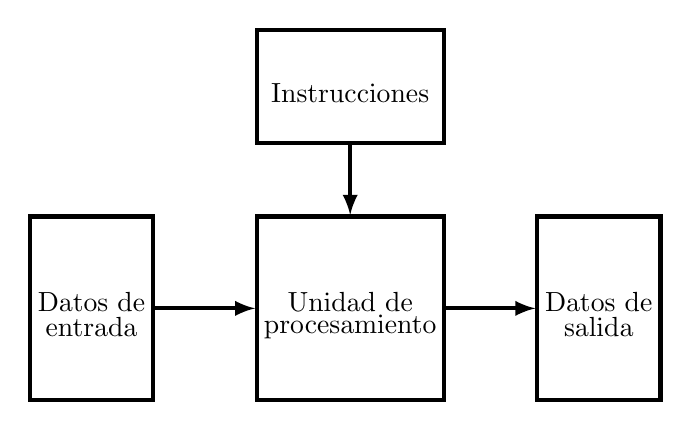
\begin{tikzpicture}
\pgftransformxscale{0.750000}
\pgftransformyscale{-0.750000}
\definecolor{dialinecolor}{rgb}{0.000000, 0.000000, 0.000000}
\pgfsetstrokecolor{dialinecolor}
\definecolor{dialinecolor}{rgb}{1.000000, 1.000000, 1.000000}
\pgfsetfillcolor{dialinecolor}
\definecolor{dialinecolor}{rgb}{1.000000, 1.000000, 1.000000}
\pgfsetfillcolor{dialinecolor}
\fill (4.707500\du,-42.000000\du)--(4.707500\du,-36.100000\du)--(8.672500\du,-36.100000\du)--(8.672500\du,-42.000000\du)--cycle;
\pgfsetlinewidth{0.100000\du}
\pgfsetdash{}{0pt}
\pgfsetdash{}{0pt}
\pgfsetmiterjoin
\definecolor{dialinecolor}{rgb}{0.000000, 0.000000, 0.000000}
\pgfsetstrokecolor{dialinecolor}
\draw (4.707500\du,-42.000000\du)--(4.707500\du,-36.100000\du)--(8.672500\du,-36.100000\du)--(8.672500\du,-42.000000\du)--cycle;
% setfont left to latex
\definecolor{dialinecolor}{rgb}{0.000000, 0.000000, 0.000000}
\pgfsetstrokecolor{dialinecolor}
\node at (6.690000\du,-39.255000\du){Datos de};
% setfont left to latex
\definecolor{dialinecolor}{rgb}{0.000000, 0.000000, 0.000000}
\pgfsetstrokecolor{dialinecolor}
\node at (6.690000\du,-38.455000\du){entrada};
\definecolor{dialinecolor}{rgb}{1.000000, 1.000000, 1.000000}
\pgfsetfillcolor{dialinecolor}
\fill (21.000000\du,-42.000000\du)--(21.000000\du,-36.100000\du)--(24.965000\du,-36.100000\du)--(24.965000\du,-42.000000\du)--cycle;
\pgfsetlinewidth{0.100000\du}
\pgfsetdash{}{0pt}
\pgfsetdash{}{0pt}
\pgfsetmiterjoin
\definecolor{dialinecolor}{rgb}{0.000000, 0.000000, 0.000000}
\pgfsetstrokecolor{dialinecolor}
\draw (21.000000\du,-42.000000\du)--(21.000000\du,-36.100000\du)--(24.965000\du,-36.100000\du)--(24.965000\du,-42.000000\du)--cycle;
% setfont left to latex
\definecolor{dialinecolor}{rgb}{0.000000, 0.000000, 0.000000}
\pgfsetstrokecolor{dialinecolor}
\node at (22.982500\du,-39.255000\du){Datos de};
% setfont left to latex
\definecolor{dialinecolor}{rgb}{0.000000, 0.000000, 0.000000}
\pgfsetstrokecolor{dialinecolor}
\node at (22.982500\du,-38.455000\du){salida};
% setfont left to latex
\definecolor{dialinecolor}{rgb}{0.000000, 0.000000, 0.000000}
\pgfsetstrokecolor{dialinecolor}
\node[anchor=west] at (22.982500\du,-39.050000\du){};
\definecolor{dialinecolor}{rgb}{1.000000, 1.000000, 1.000000}
\pgfsetfillcolor{dialinecolor}
\fill (12.000000\du,-42.000000\du)--(12.000000\du,-36.100000\du)--(18.000000\du,-36.100000\du)--(18.000000\du,-42.000000\du)--cycle;
\pgfsetlinewidth{0.100000\du}
\pgfsetdash{}{0pt}
\pgfsetdash{}{0pt}
\pgfsetmiterjoin
\definecolor{dialinecolor}{rgb}{0.000000, 0.000000, 0.000000}
\pgfsetstrokecolor{dialinecolor}
\draw (12.000000\du,-42.000000\du)--(12.000000\du,-36.100000\du)--(18.000000\du,-36.100000\du)--(18.000000\du,-42.000000\du)--cycle;
% setfont left to latex
\definecolor{dialinecolor}{rgb}{0.000000, 0.000000, 0.000000}
\pgfsetstrokecolor{dialinecolor}
\node at (15.000000\du,-39.255000\du){Unidad de};
% setfont left to latex
\definecolor{dialinecolor}{rgb}{0.000000, 0.000000, 0.000000}
\pgfsetstrokecolor{dialinecolor}
\node at (15.000000\du,-38.455000\du){procesamiento};
\definecolor{dialinecolor}{rgb}{1.000000, 1.000000, 1.000000}
\pgfsetfillcolor{dialinecolor}
\fill (12.000000\du,-48.000000\du)--(12.000000\du,-44.350000\du)--(18.000000\du,-44.350000\du)--(18.000000\du,-48.000000\du)--cycle;
\pgfsetlinewidth{0.100000\du}
\pgfsetdash{}{0pt}
\pgfsetdash{}{0pt}
\pgfsetmiterjoin
\definecolor{dialinecolor}{rgb}{0.000000, 0.000000, 0.000000}
\pgfsetstrokecolor{dialinecolor}
\draw (12.000000\du,-48.000000\du)--(12.000000\du,-44.350000\du)--(18.000000\du,-44.350000\du)--(18.000000\du,-48.000000\du)--cycle;
% setfont left to latex
\definecolor{dialinecolor}{rgb}{0.000000, 0.000000, 0.000000}
\pgfsetstrokecolor{dialinecolor}
\node at (15.000000\du,-45.980000\du){Instrucciones};
\pgfsetlinewidth{0.100000\du}
\pgfsetdash{}{0pt}
\pgfsetdash{}{0pt}
\pgfsetbuttcap
{
\definecolor{dialinecolor}{rgb}{0.000000, 0.000000, 0.000000}
\pgfsetfillcolor{dialinecolor}
% was here!!!
\pgfsetarrowsend{latex}
\definecolor{dialinecolor}{rgb}{0.000000, 0.000000, 0.000000}
\pgfsetstrokecolor{dialinecolor}
\draw (8.720837\du,-39.050000\du)--(11.950193\du,-39.050000\du);
}
\pgfsetlinewidth{0.100000\du}
\pgfsetdash{}{0pt}
\pgfsetdash{}{0pt}
\pgfsetbuttcap
{
\definecolor{dialinecolor}{rgb}{0.000000, 0.000000, 0.000000}
\pgfsetfillcolor{dialinecolor}
% was here!!!
\pgfsetarrowsend{latex}
\definecolor{dialinecolor}{rgb}{0.000000, 0.000000, 0.000000}
\pgfsetstrokecolor{dialinecolor}
\draw (15.000000\du,-44.301556\du)--(15.000000\du,-42.049771\du);
}
\pgfsetlinewidth{0.100000\du}
\pgfsetdash{}{0pt}
\pgfsetdash{}{0pt}
\pgfsetbuttcap
{
\definecolor{dialinecolor}{rgb}{0.000000, 0.000000, 0.000000}
\pgfsetfillcolor{dialinecolor}
% was here!!!
\pgfsetarrowsend{latex}
\definecolor{dialinecolor}{rgb}{0.000000, 0.000000, 0.000000}
\pgfsetstrokecolor{dialinecolor}
\draw (18.050441\du,-39.050000\du)--(20.950821\du,-39.050000\du);
}
\end{tikzpicture}

  \captionsetup{justification=centering}
  \caption{Esquema simplificado de un ``sistema de procesamiento''}
  \label{fig:C02-sistema_de_procesamiento}
\end{figure}

Estos componentes se relacionan de la forma mostrada en la figura \ref{fig:C02-sistema_de_procesamiento}. Debe notarse que los datos de entrada y las instrucciones ingresan a la unidad de procesamiento, la cual genera datos de salida como resultado de operar las instrucciones sobre los datos de entrada.\\
Los datos de entrada representan el dominio sobre el cual puede operar la unidad de procesamiento. Para definir un sistema de procesamiento debemos especificar, entonces, cuál es el dominio que puede manejar. Dicha definición deberá especificar el formato y cantidad de datos que acepta la unidad de procesamiento, así como los mecanismos para ingresarlos al sistema.\\
Las instrucciones definirán las operaciones que la unidad de procesamiento puede realizar sobre los datos de entrada. Por lo tanto, para definir un sistema de procesamiento, debemos definir qué operaciones será capaz de realizar sobre el dominio de entrada del mismo. A su vez, se debe definir la salida esperada de las instrucciones; es por eso que al definir las instrucciones estamos definiendo intrínsecamente el dominio de salida del sistema. Es importante notar que la información sobre las instrucciones también representa una entrada para el sistema, es por eso que, como en el caso de los datos de entrada, se deberá especificar formato y cantidad que acepta la unidad de procesamiento, así como los mecanismos para ingresarlas.\\
Los datos de salida representan el dominio sobre el cuál las instrucciones vuelcan el resultado de las operaciones realizadas sobre los datos de entrada. El dominio de salida, como fue notado antes, queda definido al definir las instrucciones, pero debe definirse el formato y cantidad de los mismos, así como los mecanismos necesarios para extraerlos del sistema.\\
En este contexto la unidad de procesamiento es la encargada de recibir las instrucciones y datos, ejecutar las operaciones para finalmente presentar los resultados.\\
Un microprocesadores es -en efecto- una implementación de un sistema de procesamiento. El sustento físico de dicha implementación es la microelectrónica. En las siguientes secciones de este capítulo, se repasará el marco histórico en el que surgen los microprocesadores y las arquitecturas asociadas.

\section{Perspectiva histórica}

Desde épocas remotas, el hombre se ha destacado en el mundo animal por su capacidad de modificar su entorno para resolver problemas recurrentes. Es esta capacidad la fortaleza de la especie en la naturaleza. La película ``2001: Odisea del esapcio''\footnote{2001: Odisea en el espacio es un film del año 1968 dirigida por Stanley Kubrick basada en la novela de Arthur C. Clarke.} narra, desde un enfoque particular, parte de la evolución del ser humano, o al menos la interpretación de los autores sobre la misma. En la misma, ubicándose temporalmente varios millones de años atrás, un clan de cavernícolas prehumanos intentan sobrevivir en condiciones extremas. Comen los pocos hierbajos que pueden encontrar en el desolado paisaje, hierbajos que para colmo han de compartir con una manada de tapires que habita la misma zona. La única fuente de agua del clan —un simple charco— les es arrebatada por un clan rival. Por si fuera poco, este desdichado clan vive permanentemente amenazado por un leopardo que domina la región y que de vez en cuando caza a alguno de sus miembros. En resumen: este grupo de homínidos padece hambre, frío y miedo, y parecen condenados a una segura extinción. En ese contexto, y por motivos que no vienen al caso, aparece uno de los cavernícolas contemplando el esqueleto de un animal. Parece reflexionar sobre lo que tiene delante, como si estuviese viéndolo desde una nueva perspectiva. Hay algo nuevo en aquellos huesos. Algo que hasta entonces ni él ni ninguno de sus congéneres habían visto. Los huesos que hay tirados por el suelo pueden ser usados. El cavernícola toma el más robusto de los huesos y empieza a golpear el esqueleto; primero con precaución, más tarde con fuerza, hasta que termina consumido por un frenesí violento. Este cavernícola acaba de descubrir el primer arma —la primera herramienta— de la historia. O dicho de otro modo, acaba de aparecer el primer ser humano sobre la faz de la tierra. Gracias al uso del hueso —o de herramientas similares como palos o piedras— el clan que estaba a punto de extinguirse descubre que puede cazar a los tapires con los que convive y comérselos. Así que sus problemas de hambre han terminado. También gracias a sus armas pueden atacar al clan rival y recuperar el charco de agua, lo que soluciona también sus problemas de sed. Y deducimos que serán capaces incluso de defenderse del peligroso leopardo. Los miembros del clan ya no son prehumanos indefensos; ahora son humanos armados.\\
Esta cita cinematográfica pretende graficar la diferenciación del ser humano en la cadena alimenticia. Gracias al poder de la observación y el razonamiento hemos sido capaces de modificar nuestro entorno para asegurar la supervivencia de la especie en un mundo en el que la misma se encontraba en clara desventaja. En este contexto, el ser humano ha sido capaz de generar un desarollo tecnológico, que hoy en día es vertiginoso.\\

\subsection{La máquina de Turing}

Alan Mathison Turing\footnote{Alan Mathison Turing (23 June 1912 – 7 June 1954): Típicamente considerado el padtre de las ciencias de la computación y de la inteligencia artificial, fue un biólogo, matemático, lógico, científico de la computación y de la criptografía que formalizó los conceptos de algoritmo y computación mediante la ``Máquina de Turing'', que es un modulo de una computadora de propósito general} es considerado el padre de la computación y la inteligencia artificial. Sus trabajos en el campo de la computación se remontan al año 1936 cuando publica un \emph{paper} llamado ``On computable Numbers, with an Application to the Entscheidungsproblem''.

\subsection{La revolución digital}

La revolución digital es considerada la tercera revolución industrial. Sus comienzos se remontan a fines de los años 50. La adopción y proliferación de las computadoras digitales y el mantenimiento de registros digitales de información son las características que la definen. De manera implícita, esta revolución está relacionada con los cambios radicales provocados por la computación y las tecnologías de telecomunicaciones. Esta revolución dió orígen a lo que hoy conocemos como la ``era de la información''. En el corazón de este proceso encontramos dos componentes tecnológicas. Por un lado está la teoría, que puede remontarse a los primeros análisis matemáticos de la lógica, como el álgebra de Boole introducida por primera vez en un pequeño folleto publicado en 1847 bajo el nombre \emph{The Mathematical Analisis of Logic} y la posterior publicación del libro \emph{An Investigation of the Laws of Thought on Which are Founded the Mathematical Theories of Logic and Probabilities}, publicado en 1854. En estas publicaciónes George Boole\footnote{Nota sobre George Boole} pretendió utilizar técnicas algebraicas para tratar expresiones de la lógica proposicional. En la actualidad, el álgebra de Boole se aplica de forma generalizada en el ámbito del diseño electrónico. Claude Shannon\footnote{Nota sobre Claude Shannon} fué el primero en aplicarla en el diseño de circuitos de conmutación eléctrica biestables, en 1948. Por el otro lado, se encuentra la revolución del silicio y la producción en masa y uso generalizado de circuitos lógicos digitales que permitieron el desarrollo en gran escala de circuitos electrónicos que implementan funciones lógicas basados en los desarrollos de Boole. Aproximadamente cien años pasaron desde que Boole publicó su teoría, hasta que la tecnología encontró el camino para implementar esos conocimientos de forma práctica y útil. La invención del transistor data del año 1947. En la figura \ref{fig:C02-primer_transistor} se muestra una imágen de una réplica de este primer transistor de la historia. Este invento fué el que permitió la creación de equipos digitales avanzados. En el contexto de la lógica digital, los transistores son utilizados como llaves de conmutación que permiten o no el paso de una señal eléctrica al ser excitados por otra señal. Previo a los transistores, la lógica era implementada con componentes electromecánicos y válvulas termoiónicas de vacío; tecnologías que por su naturaleza eran de dimensiones y consumos energéticos elevados y poco fiables. Para poner esta problemática en perspectiva, comparamos la primer computadora de propósito general electrónica, llamada ENIAC\footnote{Descripción de la ENIAC} implementada con 18000 válvulas, con un consumo de $160\,\mathrm{kW}$, capaz de realizar $5000\,\mathrm{sumas/s}$, $385\,\mathrm{multiplicaciones/s}$, con 5 millones de soldaduras y un peso de $30\,\mathrm{Tn}$, contra un procesador Intel Core I7 que permite $177000\,\mathrm{MIPS}$ con un consumo de aproximadamente $100\,\mathrm{W}$, es decir, 35 millones de veces más rápido. Para hacer la misma cantidad de sumas por segundo se requerirían $5\,\mathrm{GW}$ con la ENIAC; considerar que la capacidad actual instalada en argentina es de $30\,\mathrm{GW}$.
\begin{figure}
  \centering
%  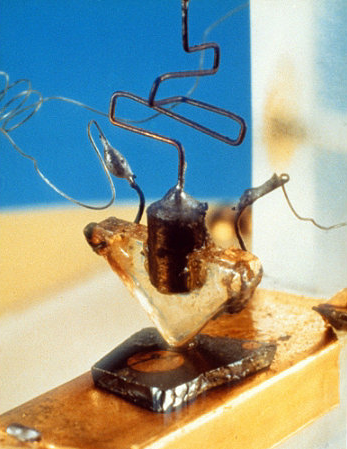
\includegraphics[width=11cm]{./figures/C02-MIMO_diagram_01
  \includegraphics[scale=0.5]{./figures/C02-primer_transistor}
  \captionsetup{justification=centering}
  \caption{Primer transistor desarrollado por John Bardeen y Walter Brattain bajo la dirección de William Shockley en los Laboratorios Bell de AT\&T en el año 1947}.
  \label{fig:C02-primer_transistor}
\end{figure}

\subsection{Silicio, dispositivos semiconductores y transistores}

Los semiconductores son materiales, que como bien indica su nombre, no son del todo conductores. En ellos, la capacidad de conducir una corriente eléctrica puede ser manipulada de diversas maneras. En 1931 Wolfgang Pauli -quien en 1945 fue premiado con el Nobel de Física- enunció: ``Uno no debería trabajar en semiconductores, eso es un lío deleznable, quién sabe si realmente existen''. Nada más alejado de la realidad que hoy nos rodea. Los materiales semiconductores permitieron la creación de los transistores y posteriormente los circuitos integrados, dispositivos que iniciaron la revolución digital. Los primeros dispositivos fueron fabricados sobre germanio y arsenurio de galio. Incluso, el primer circuito integrado, fue realizado en germanio. Pero fue el 
silicio el material que realmente revolucionó la industria, por su alta disponibilidad en la naturaleza y relativa fácil manipulación para la fabricación de dispositivos semiconductores en circuitos integrados. Puede afirmarse que el silicio es uno de los materiales mejor conocidos por el ser humano. Hace más de 50 años que se lo estudia en detalle para mejorar la tecnología, logrando importantes avances. También puede afirmarse que el los transistores hoy en día es el bien más abundante en el mundo. Una comparativa del año 2012 muestra que durante año se produjeron en el órden de $10^{17}$ granos de arroz en la tierra, mientras que en el mismo período en se produjeron en el órden de $10^{19}$ transistores, según declaraciones de la \emph{Semiconductor Industry Asociation} de los Estados Unidos de América. La clave de semejante número en la producción son los circuitos integrados.

\subsection{Circuitos integrados y tencología CMOS}

En la figura \ref{fig:C02-primer_circuito_integrado} puede verse el primer circuito integrado de la historia. Medía aproximadamente media pulgada de ancho e implementaba dos transistores montados en una barra de germanio. Nace así el concepto del \emph{chip} o \emph{microchip}: en inglés, \emph{chip} significa ``corte o fracción pequeño de un material duro'' directamente relacionado con la técnica de fabricación de circuitos integrados donde, a grandes rasgos, una barra cilíndrica de cristal de silicio puro, es cortada en muy delgadas láminas en forma de discos, sobre las cuales se ``imprimen'' los circuitos integrados, repitiendo el mismo patrón múltiples veces en un mismo disco para finalmente cortar ese disco en diminutos fragmentos que contienen el diseño. La evolución de las técnicas de fabricación permitieron integrar en un mismo \emph{chip} de silicio más de un dispositivo, permitiendo implementar circuitos relativamente complejos en una pequeña área de silicio, disminuyendo así los riesgos de fallas por interconexión entre dispositivos. A su vez, las técnicas de fabricación evolucionaron permitiendo escalar el tamaño de los dispositivos fabricados incrementando la cuenta de dispositivos integrados por unidad de área. Como consecuencia buscada de disminuir el tamaño de los dispositivos, se logró aumentar la velocidad máxima de conmutación que los mismos pueden lograr, redundando en generar lógica cada vez más compleja y rápida en un mismo \emph{chip}. En simultáneo con estos avances se comenzaron a fabricar transistores MOS\footnote{Transistor Metal-Oxido-Semiconductor: Nota}, transistores de efecto de campo eléctrico, que como gran ventaja sobre los ``antiguos'' transistores de juntura, evitaban la disipación de potencia al mantenerse en un estado definido (encendido o apagado), es decir que sólo disipaban potencia al cambiar de estado. Es así que en el año 1978 aparece la tecnología CMOS\footnote{CMOS: Nota. Complementariedad. Sólo utiliza MOSFET-N y MOSFET-P para implementar cualquier función} la cual permitió elevar el nivel de integración en forma masiva, manteniendo bajos niveles de disipación de potencia. Debido a la relativa sencillez geométrica del diseño de los transistores MOS, se pueden reutilizar diseños escalándolos para las nuevas generaciones de tecnología. El 19 de abril de 1965 Gordon E. Moore\footnote{Nota sobre Gordon E. Moore}, cofundador de Intel\footnote{Nota sobre Intel}, estableció de forma empírica que la cantidad de dispositivos integrados en un circuito integrado se duplicaría cada año. Más tarde, en 1975, modificó su propia ley al corroborar que el ritmo bajaría, y que la capacidad de integración no se duplicaría cada 12 meses sino cada 24 meses aproximadamente. Esta progresión de crecimiento exponencial, duplicar la capacidad de los circuitos integrados cada dos años, es lo que se denomina ley de Moore. Sin embargo, en 2007 el propio Moore determinó una fecha de caducidad: ``Mi ley dejará de cumplirse dentro de 10 o 15 años'', no obstante también aseveró que una nueva tecnología vendrá a suplir a la actual. El cumplimiento se ha podido constatar hasta hoy.

\begin{figure}
  \centering
  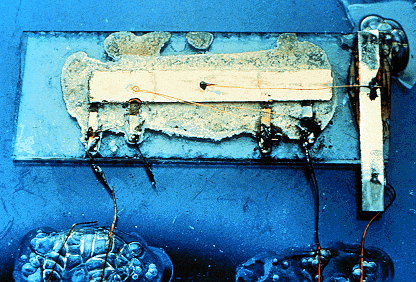
\includegraphics[scale=0.5]{./figures/C02-primer_circuito_integrado}
  \captionsetup{justification=centering}
  \caption{Primer circuito integrado presentado por Texas Instruments, Inc. el 12 de Septiembre de 1958}
  \label{fig:C02-primer_circuito_integrado}
\end{figure}

La ley de Moore, no es una ley en el sentido científico, sino más bien una observación del ritmo de avance de la industria de aquellos momentos. Al momento de publicar esas declaraciones, Moore trabajaba en los Laboratorios de Fairchild Semiconductor, donde trabajaba junto a Robert Noyce. Ellos fueron los fundadores de Intel en 1968. El ritmo de crecimiento de la insdustria de los Semiconductores dió lugar así, entre otras cosas, a la creación de los microprocesadores.

\subsection{Microprocesadores}

Los microprocesadores surgen como consecuencia del alto nivel de integración y complejidad que la tencología de circuitos integrados permitieron alcanzar. Una computadora digital, podía ser construída en uno o algunos pocos \emph{chips} de circuitos integrados. Los primeros diseños de microprocesadores propiamente dichos datan de fines de los años 60. Dentro de este contexto aparece el término \emph{Central Processing Unit} (Unidad Central de Procesamiento) o CPU, que es la parte de la máquina encargada de tomar los datos de entrada y las intrucciones y generar los resultados, dentro del esquema del sistema de procesamiento planteado al principio de éste capítulo. El microprocesador integra además otros componentes y funcionalidades y se vale de ciertos periféricos que pueden estar o no integrados en el mismo circuito, como por ejemplo, memorias de sólo lectura (\emph{Read Only Memory} o ROM\footnote{Nota sobre ROM}) y memorias de acceso aleatorio (Random Access Memories o RAM\footnote{Nota sobre RAM}) y dispositivos de entrada / salida (\emph{I/O, input output devices}. El diseño de arquitecturas de microprocesarores, como todo proceso de innovación tecnológica, no estuvo exento de discusiones y distintas vertientes y prácticas a seguir. Los primeros diseños de los que se tenga registro en órden cronológico, fueron:

\subsubsection{CADC}

En 1968, la armada de los Estados Unidos le encomienda a la empresa Garret Air Research\footnote{Nota sobre Garret AiResearch} la producción de una computadora digital que pudiera competir con los sistemas electromecánicos que estaban bajo desarrollo para los sistemas de control de vuelo del nuevo avión de combate F-14 Tomcat. El diseño fue completado en 1970 y utilizaba un conjunto de chips (\emph{chipset}) MOS como CPU, siendo aproximadamente 20 veces más pequeño que su contraparte electromecánica y a su vez, mucho más confiable. Este diseño fue utilizado en todos los primeros modelos de Tomcat. La armada se rehusó a publicar el diseño hasta 1997, es por eso que la CADC (Central Air Data Computer) y su \emph{chipset} asociado MP944 no son muy conocidos y no son considerados en la mayoría de la bibliografía reelevante y es a partir de ese momento en que son reconocidos como los primeros diseños válidos de microprocesadores, y no sólo eso, si no que también son la primera especie de \emph{Digital Signal Processor} (Procesador de Señales Digitales) o DSP\footnote{Nota sobre DSP} puesto que además de las funciones de microprocesador, implementaba la funcionalidad de medir variables como altitud, velocidad vertical y número de \emph{mach}\footnote{Nota sobre Mach number} a partir de datos de sensores pitot, presión estática y temperatura. Los responsables del diseño fueron Ray Holt\footnote{Nota sobre Ray Holt} y Steve Geller\footnote{Nota sobre Steve Geller}

\begin{figure}
  \centering
  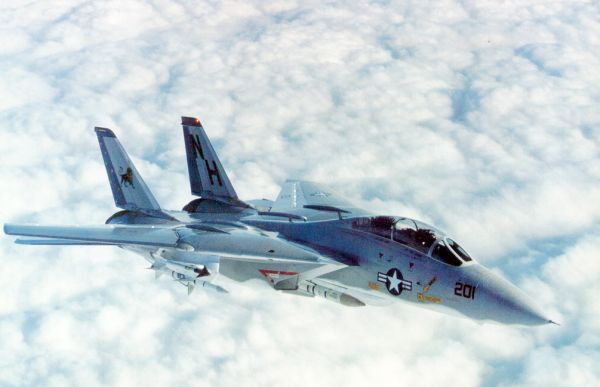
\includegraphics[scale=0.5]{./figures/C02-f14_tomcat}
  \captionsetup{justification=centering}
  \caption{Grumman F14 Tomcat, avión de combate de la US Navy cuyos sistemas de vuelo eran controlados por la CADC.}
  \label{fig:C02-f14_tomcat}
\end{figure}


\subsubsection{Four-Phase Systems AL1}

Un diseño de Lee Boysel\footnote{Nota sobre Lee Boysel} que data del año 1969 dentro de Texas Instruments\footnote{Nota sobre TI}, era un componente de una implementación en partes de un microprocesador de 24 bits, compuesto por tres chips iguales: AL1. Durante un juicio por patentes, se demostró que una sóla AL1 junto con memorias ROM y RAM e I/O era capaz de funcionar como CPU.

\begin{figure}
  \centering
  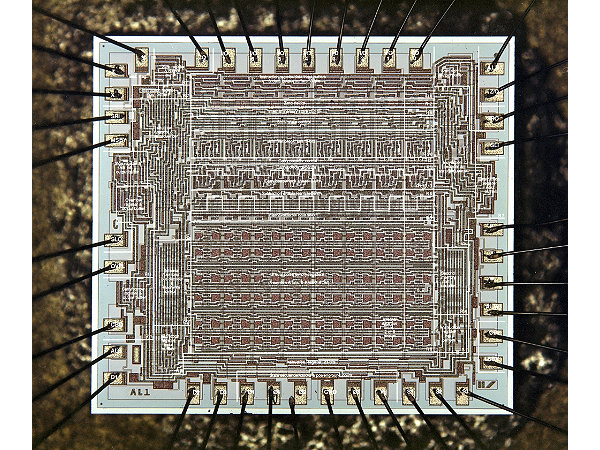
\includegraphics[scale=0.5]{./figures/C02-al1}
  \captionsetup{justification=centering}
  \caption{Imágen microscópica de la AL1 desarrollada por Four-Phase Systems Inc..}
  \label{fig:C02-al1}
\end{figure}


\subsubsection{Pico/General Instruments}

En 1971, Pico y General Instruments (GI) colaboraron en el diseño de circuitos integrados con el objetivo de fabricar una implementación de un diseño de \emph{chip} único para la calculadora Monroe/Litton Royal Digital III Calcultator. Integraba en el mismo \emph{chip}, memoria ROM y RAM llamado PICO1/GI250. Pico era un emprendimiento de cinco ingenieros de diseño de GI, que tenían la visión de crear esta arquitectura en un único \emph{chip}. Contaban con experiencia previa en diseños de \emph{chipsets} tanto de GI como de Marconi-Elliot\footnote{Nota sobre Marconi-Elliot}. Algunos de ellos habían trabajado para Elliot Automation para crear una computadora de 8 bits en tecnología MOS, y habían ayudado a establecer un laboratorio de investigación en tecnologías MOS en Escocia en el año 1967. El mercado de las calculadoras estaba en pleno auge, con lo cuál estos diseños supusieron un éxito comercial para Pico y GI. GI, por su parte continuó con la innovación en microprocesadores microcontroladores\footnote{Nota sobre diferencia entre microprocesador y microcontrolador} y la división GI Microelectronics se convirtió en 1987 en Microchip PIC microcontroller.

\begin{figure}
  \centering
  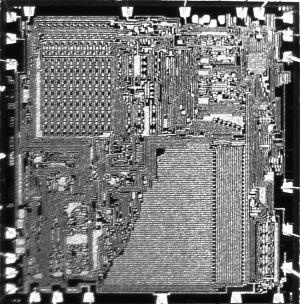
\includegraphics[scale=0.5]{./figures/C02-pico1_gi250}
  \captionsetup{justification=centering}
  \caption{Imágen microscópica del PICO1/GI250- Desarrollo colaborativo entre Pico y General Instruments de \emph{chip} único para la Monroe/Litton Royal Digital III Calcultator.}
  \label{fig:C02-pico1_gi250}
\end{figure}

\subsubsection{Intel 4004}

El Intel 4004 es generalmente el reconocido como el primer microprocesador comercial disponible en el mercado. El primer anuncio respecto de este dispositivo data del 15 de Noviembre de 1971, en la publicación Electronic News\footnote{Nota sobre Electronic News}. El diseño nace a partir del requerimiento de una compañía japonesa fabricante de calculadoras llamado Busicom\footnote{Nota sobre Busicom}, que le encomienda a Intel la tarea de desarrollar un \emph{chipset} para calculadoras de escritorio de alto rendimiento. El diseño original requerido por Busicom especificaba un \emph{chipset} compuesto por 7 \emph{chips} diferentes para la realización de una CPU de propósito específico cuyo programa estuviera almacenado en una ROM y sus datos guardados memoria de lectura y escritura implementada con registros de desplazamiento. Intel le asignó el proyecto a Ted Hoff\footnote{Nota sobre Ted Hoff}, quien propuso simplificar el diseño utilizando almacenamiento en memoria RAM dinámica y una arquitectura de CPU de propósito general. El diseño propuesto por Hoff implementaba la solución en 4 \emph{chips}: uno de ROM para almacenar el programa, uno de RAM dinámica para almacenar los datos, un dispositivo sencillo de I/O y una CPU de 4 bits. A pesar de no ser específicamente un diseñador de circuitos integrados, el supuso que se podía integrar todo el CPU en un único \emph{chip}. Estas especificaciones surgieron de la interacción de Hoff con un empleado a su cargo, el ingeniero de software llamado Stanley Mazor\footnote{Nota sobre Stanley Mazor} y un ingeniero de Busicom llamado Masatoshi Shima\footnote{Nota sobre Masatoshi Shima}. Este proyecto se llamó MCS-4 y no fué hasta que Intel contratara al italiano Federico Faggin\footnote{Nota sobre Federico Faggin} que empezó a tomar su forma definitiva. Faggin venía de desarollar en 1968 en Fairchild Semiconductor una teconología de compuertas de silicio (SGT o \emph{Silicon Gate Technology}\footnote{Nota sobre SGT, o también llamada Self-aligned Gate}), técnica que se sigue aplicando hoy en día. Faggin también era responsable del desarrollo de la técnica llamada \emph{Random Logic} que permitió la síntesis de descripciones complejas de lógica en hardware sencillo, como compuertas AND y OR. En el momento en el que se estaba desarrollando el proyecto MCS-4, el responsable del área de diseño de MOS de Intel era Leslie L. Vadász, cuya atención estaba enfocada en el mercado de memorias. Fue gracias a esto que le otorgó el liderazgo del proyecto MCS-4 a Faggin, quien fue finalmente el responsable de llevar el proyecto hasta la concepción final del 4004 gracias a la aplicación de las técnicas de diseño y fabricación antes mencionadas. Las primeras unidades del 4004 fueron entregadas a Busicom en Marzo de 1971.

\begin{figure}
  \centering
  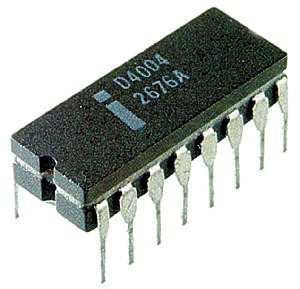
\includegraphics[scale=0.5]{./figures/C02-intel_4004}
  \captionsetup{justification=centering}
  \caption{Encapsulado del Intel 4004; que es considerado el primer microprocesador comercial en ser introducido en el mercado.}
  \label{fig:C02-intel_4004}
\end{figure}

\section{Evolución hacia las arquitecturas modernas}

El concepto moderno de las arquitecturas se basa en las máquinas que almacenan tanto el programa que se ejecuta, como los datos que se manjan en memoria de lectura-escritura (\emph{Stored-Program digital computer}). Esto las diferencia de las primeras implementaciones de los años 40, tales como Colossus\footnote{Nota sobre Colossus} y la ENIAC.\\
En esta sección se estudian las distintas clasificaciones de arquitecturas existentes hoy en día. Luego se detallarán diversas arquitecturas existentes y se las enmarcará dentro de dichas clasificaciones.

\subsection{Clasificación de las arquitecturas según el acceso a la memoria de instrucciones y datos}

Las instrucciones que ejecuta el procesador, al igual que los datos del programa en ejecución, deben residir en la memoria. De este hecho se desprende que existen -al menos- dos tipos de memorias: de instrucciones, y de datos. El acceso a estas dos memorias puede realizarse a través del mismo \emph{bus}\footnote{Bus: definir bus} o con \emph{buses} separados. Los nombres que la historia les ha provisto a estos dos posibles enfoques, son \emph{von Neumann} para las arquitecturas de \emph{bus} único y \emph{Harvard} para aquellas de \emph{buses} separados.

\subsubsection{Arquitectura von Neumann}

También conocida como modelo de von Neumann y arquitectura Princeton, este tipo de arquitectura debe su nombre a John von Neumann\footnote{Nota sobre el chango}, quién en el año 1945 describió en el documento inconcluso, cuya carátula puede verse en la figura \ref{fig:C02-von_neumann_first_draft} y conocido como \emph{First Draft of a Report on the EDVAC}\cite{vonNeumann}, una arquitectura de computadora electrónica digital para ser implementada con válvulas de vacío. Ésta fue la primera publicación dónde se describe el diseño lógico de una computadora que utilizase el concepto de \emph{stored-program} o programa almacenado. Este diseño, tal como fue llamado por el propio von Neumann, \emph{very high speed automatic digital computing system} o sistema automático digital de cómputo de muy alta velocidad, estaba dividido en 6 componentes:
\begin{itemize}
  \item CA: \emph{central arithmetic} o aritmética central
  \item CC: \emph{central control} o control central
  \item M: \emph{memory} o memoria
  \item I: \emph{input} o entrada
  \item O: \emph{output} o salida
  \item R: \emph{external memory} o memoria externa
\end{itemize}
\begin{figure}
  \centering
  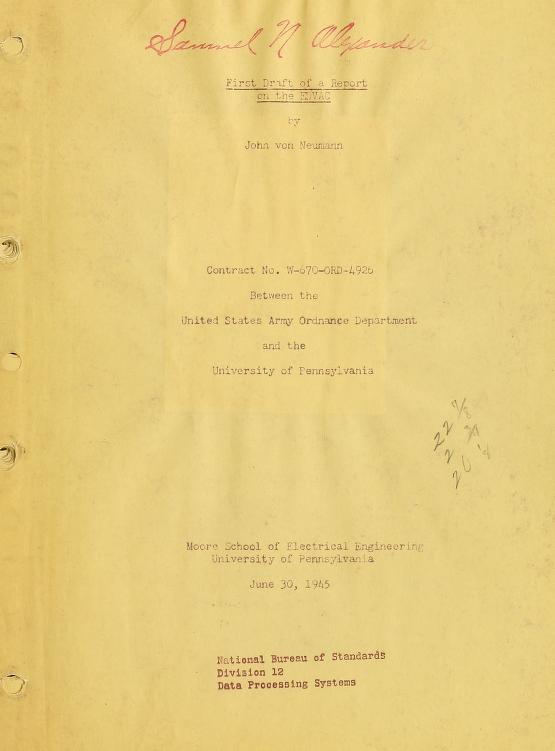
\includegraphics[scale=0.25]{./figures/C02-von_neumann_first_draft}
  \captionsetup{justification=centering}
  \caption{Carátula del escrito de von Neumann First Draft of a Report on the EDVAC}
  \label{fig:C02-von_neumann_first_draft}
\end{figure}
La memoria almacena tanto números (datos) como órdenes (instrucciones).
La aritmética central podía realizar sumas, restas, multiplicaciones, divisiones y raices cuadradas. Otras operaciones matemáticas, como logaritmos y funciones trigonométricas se debían realizar utilizando tablas de búsqueda e interpolaciones, posiblemente bicuadráticas. Una decisión de diseño establecida en el documento estableció que multiplicaciones y divisiones podían realizarse mediante tablas logarítmicas, pero para poder mantener dichas tablas pequeñas debería utilizarse interpolaciones, lo cuál a su vez necesita de multiplicaciones, aunque de menor precisión.\\
Los números se represetaban mediante notación binaria. Estimó que 27 dígitos binarios\footnote{En el documento se hace meción a dígitos binarios y no a \emph{bits}, término que fue acuñado en 1948 por Claude Shannon} deberían ser suficientes, pero redondéo a 30 dígitos, más uno de signo y otro para diferenciar los números de las órdenes, resultando en palabras de 32 dígitos binarios. La aritmética utilizada era complemento a dos para simplificar la operación de resta. Para la multiplicación y la división, propuso ubicar el punto binario luego del bit de signo, lo que implica que el dominio de los operandos y resultados está en el rango -1 a 1, y por lo tanto, los datos y resultados de los programas deberían ser escalados acordemente.\\
En cuanto al diseño de los circuitos, estableció que deberían utilizarse válvulas de vacío, dejando de lado los relé, dada a la mayor velocidad provista por las primeras. Otras sugerencias involucraban mantener al sistema de cómputo lo más sencillo posible, evitando cualquier tipo de optimización de performance mediante la superposición de operaciones. Las operaciones aritméticas debían realizarse de a un dígito binario a la vez. Estimó el tiempo de la suma de dos dígitos binarios en un microsegundo, por lo tanto la multiplicación de dos números representados por 30 dígitos binarios deberí realizarse en aproximadamente $30^{20}$ microsegundos; lo cuál era mucho más rápido que el tiempo de cualquier dispositivo de cálculo del momento. El diseño estaba basado en lo que von Neumann llamó ``elemento E'', basándose en el modelo biológico de las neuronas, pero implementado de forma digital planteando que podrían ser fabricados mediante una o dos válvulas. En términos modernos, la forma más sencilla del ``elemento E'' es una compuerta \emph{AND} de dos entradas, con una de sus entradas invertidas, llamada ``entrada de inhibición''. Al agregar más entradas a este dispositivo, se establecía un nivel de umbral, el cual al ser superado por la suma de una determinada cantidad de entradas generaba una salida en tanto y en cuanto no se excitara la entrada de inhibición. También estableció que dichos elementos de múltiples entradas podían ser construidos utilizando combinaciones de la versión elemental, pero recomendaba implementarlos por completo utilizando así menos válvulas de vacío con el objetivo de lograr circuitos más sencillos y rápidos, principio que hoy en día se mantiene vigente.\\
Toda función lógica arbitraria, podía implentarse, entonces, a partir de dichos ``elementos E''. Demostró en este trabajo, cómo implementar circuitos que implementaban las funciones aritméticas, así como elementos de memoria y circuitos de control, sin referirse en ningún momento al término de ``lógica binaria''.\\
Los ciruitos debían ser sincrónicos, obteniendo la señal de reloj a partir de un circuito oscilador implementado con válvulas y posiblemente controlado mediante cristales osciladores. Los diagramas lógicos incluían los tiempos de demora representados mediante una flecha. Estimó que la velocidad a la que se movía un pulso eléctrico en un cable era de $300 mts/microsegundo$, por lo tanto no debería generar problemas hasta obtener velocidades de reloj de $100MHz$. Tambíen menciona pero no desarrolla la necesidad de contar con mecanismos de detección y correción.\\
En cuanto a la memoria, que es donde entra la clasificación discutida en esta sección, von Neumann estableció que la memoria es uniforme, conteniendo tanto los números (datos) como las órdenes (instrucciones). Citando su trabajo:\\
``El dispositivo requiere una memoria considerable. A pesar de que pareciese que distintas partes de la memoria tiene que realizar funciones que difieren en su naturaleza y considerablemente en su propósito, resulta tentador tratar a toda la memoria con un sólo órgano, y hacer que sus partes sean tan intercambiables como sea posible para todas las funciones que deban realizar'' \cite[sección, 2.5]{vonNeumann}\\
``Lás órdenes recibidas por CC vienen de M, es decir, el mismo lugar donde se almacenan los datos numéricos''\cite[sección, 14.0]{vonNeumann}.\\
Él concluyó que la memoria sería el subsistema más grande y abarcativo de la máquina. Basándose en diversos problemas matemáticos, incluyendo la resolución de ecuaciones diferenciales parciales y ordinarias, ordenamientos y experimentos probabilísticos, estimó que se necesitaba espacio para almacenar 8192 palabras de 32 dígitos binarios para los datos, y algunos cientos de palabras para  almacenar las órdenes. Para la implementación de memoria, propuso dos tipos de memoria rápida, \emph{delay line memory} e \emph{iconoscope}. Con estas implementaciones planteó que la memoria debía ser direccionable por palabras y para sortear los problemas de demora asociados a la lectura de estas memorias, organizó las mismas en 256 conjuntos de 1024 dígitos binarios, o sea 32 palabras, logrando así direccionar los conjuntos con 8 dígitos binarios y las palabras con 5 utilizando, entonces, 13 dígitos binarios en total para el direccionamiento completo.\\
En su trabajo también estableció el formato de las órdenes, al cual llamó ``código''. Los tipos de órdenes incuyeron las operaciones aritméticas básicas, así como el movimiento de palabras entre CA y M (análogas a las instrucciones \emph{load} y \emph{store} de hoy en día que veremos más adelante), una órden que elegía entre dos números basado en el signo del resultado de una operación previa (análoga a una instrucción \emph{branch}), órdenes para controlar la entrada y salida de datos y para indicarle a la CC que debía tomar instrucciones desde otra sección de M (análoga a un \emph{jump}). Determinó, asimismo, la cantidad de dígitos binarios necesarios para necesarios para los distintos tipos de órdenes, sugirió lo que llamó ``órdenes inmediatas'', donde la siguiente palabra  se trata del operando (lo cual también tiene una anagolía con ciertos conjuntos de instrucciones actuales) y dejó planteado si era deseable dejar dígitos sin especificar para propósitos futuros y mayor direccionamiento de memoria.

\subsubsection{Arquitectura Harvard}

Este tipo de arquitectura, ve sus orígenes en un desarrollo propuesto por el Dr. Howard Aiken\footnote{Nota sobre Aiken} en la universidad de Harvard en el año 1937 basado en el trabajo llamado \emph{Analytical Engine}\footnote{Nota sobre Analytical Engine} de Charles Babage\footnote{Nota sobre el tipo}. El desarrollo fue llevado al cabo por IBM\footnote{Nota sobre IBM} y se trataba de una máquina de cálculo llamada \emph{Automatic Sequence Controlled Calculator - Harvard Mark I} entregado a la universidad el 24 de agosto de 1944. A diferencia de la máquina propuesta (posteriormente) por von Neumann, ésta era una máquina electromecánica construida con llaves, relés, engranajes y embreagues. Constaba de 765000 componentes electromecánicos, cientos de millas de cableado, un peso de 4.5 Ton. y un consumo de potencia de 3.7 kW. Para el ingreso de datos, contaba con 60 conjuntos de 24 llaves rotativas que permitían ingresar números decimales. Podía almacenar hast 72 números de hasta 23 dígitos decimales. En un segundo era capaz de realizar 3 sumas o restas. La multiplicación tardaba 6 segundos y una división 13.5 segundos. El calculo de funciones logarítmicas o trigonométricas utilizaba más de un minuto. Las instrucciones eran ingresadas a través de cintas perforadas de 24 canales (en la figura \ref{fig:C02-mark_i_instruction_tape} se puede ver una cinta con instrucciones de esta máquina). Otra cinta podía ser utilizada para el ingreso de datos, pero utilizando un formato distinto al de las instrucciones; estas no podían ser ejecutadas desde los registros de almacenamiento. Esta separación entre datos e instrucciones es lo que se conoce como arquitectura Harvard y que la diferencia de la arquitectura von Neumann. El formato de las instrucciones definía tres campos en ocho canales separados. Cada acumulador, cada conjunto de switches, y los registros asociados a la entrada y salida y las unidades aritméticas tenían asignado un índice único. Estos números eran representados en formato binario en la cinta perforada de control, siendo el primer campo el índice del resultado de la operación, el segundo el orígen del dato para la operación y el tercero el código que representa la operación a realizar. Una particularidad de ésta primera versión es que no tenía instrucción para el salto condicional en el programa. Por lo tanto, los programas complejos debían ser largos y los ``loops'' se implementaban uniendo físicamente el final de la cinta perforada del programa con el principio.\\
\begin{figure}
  \centering
  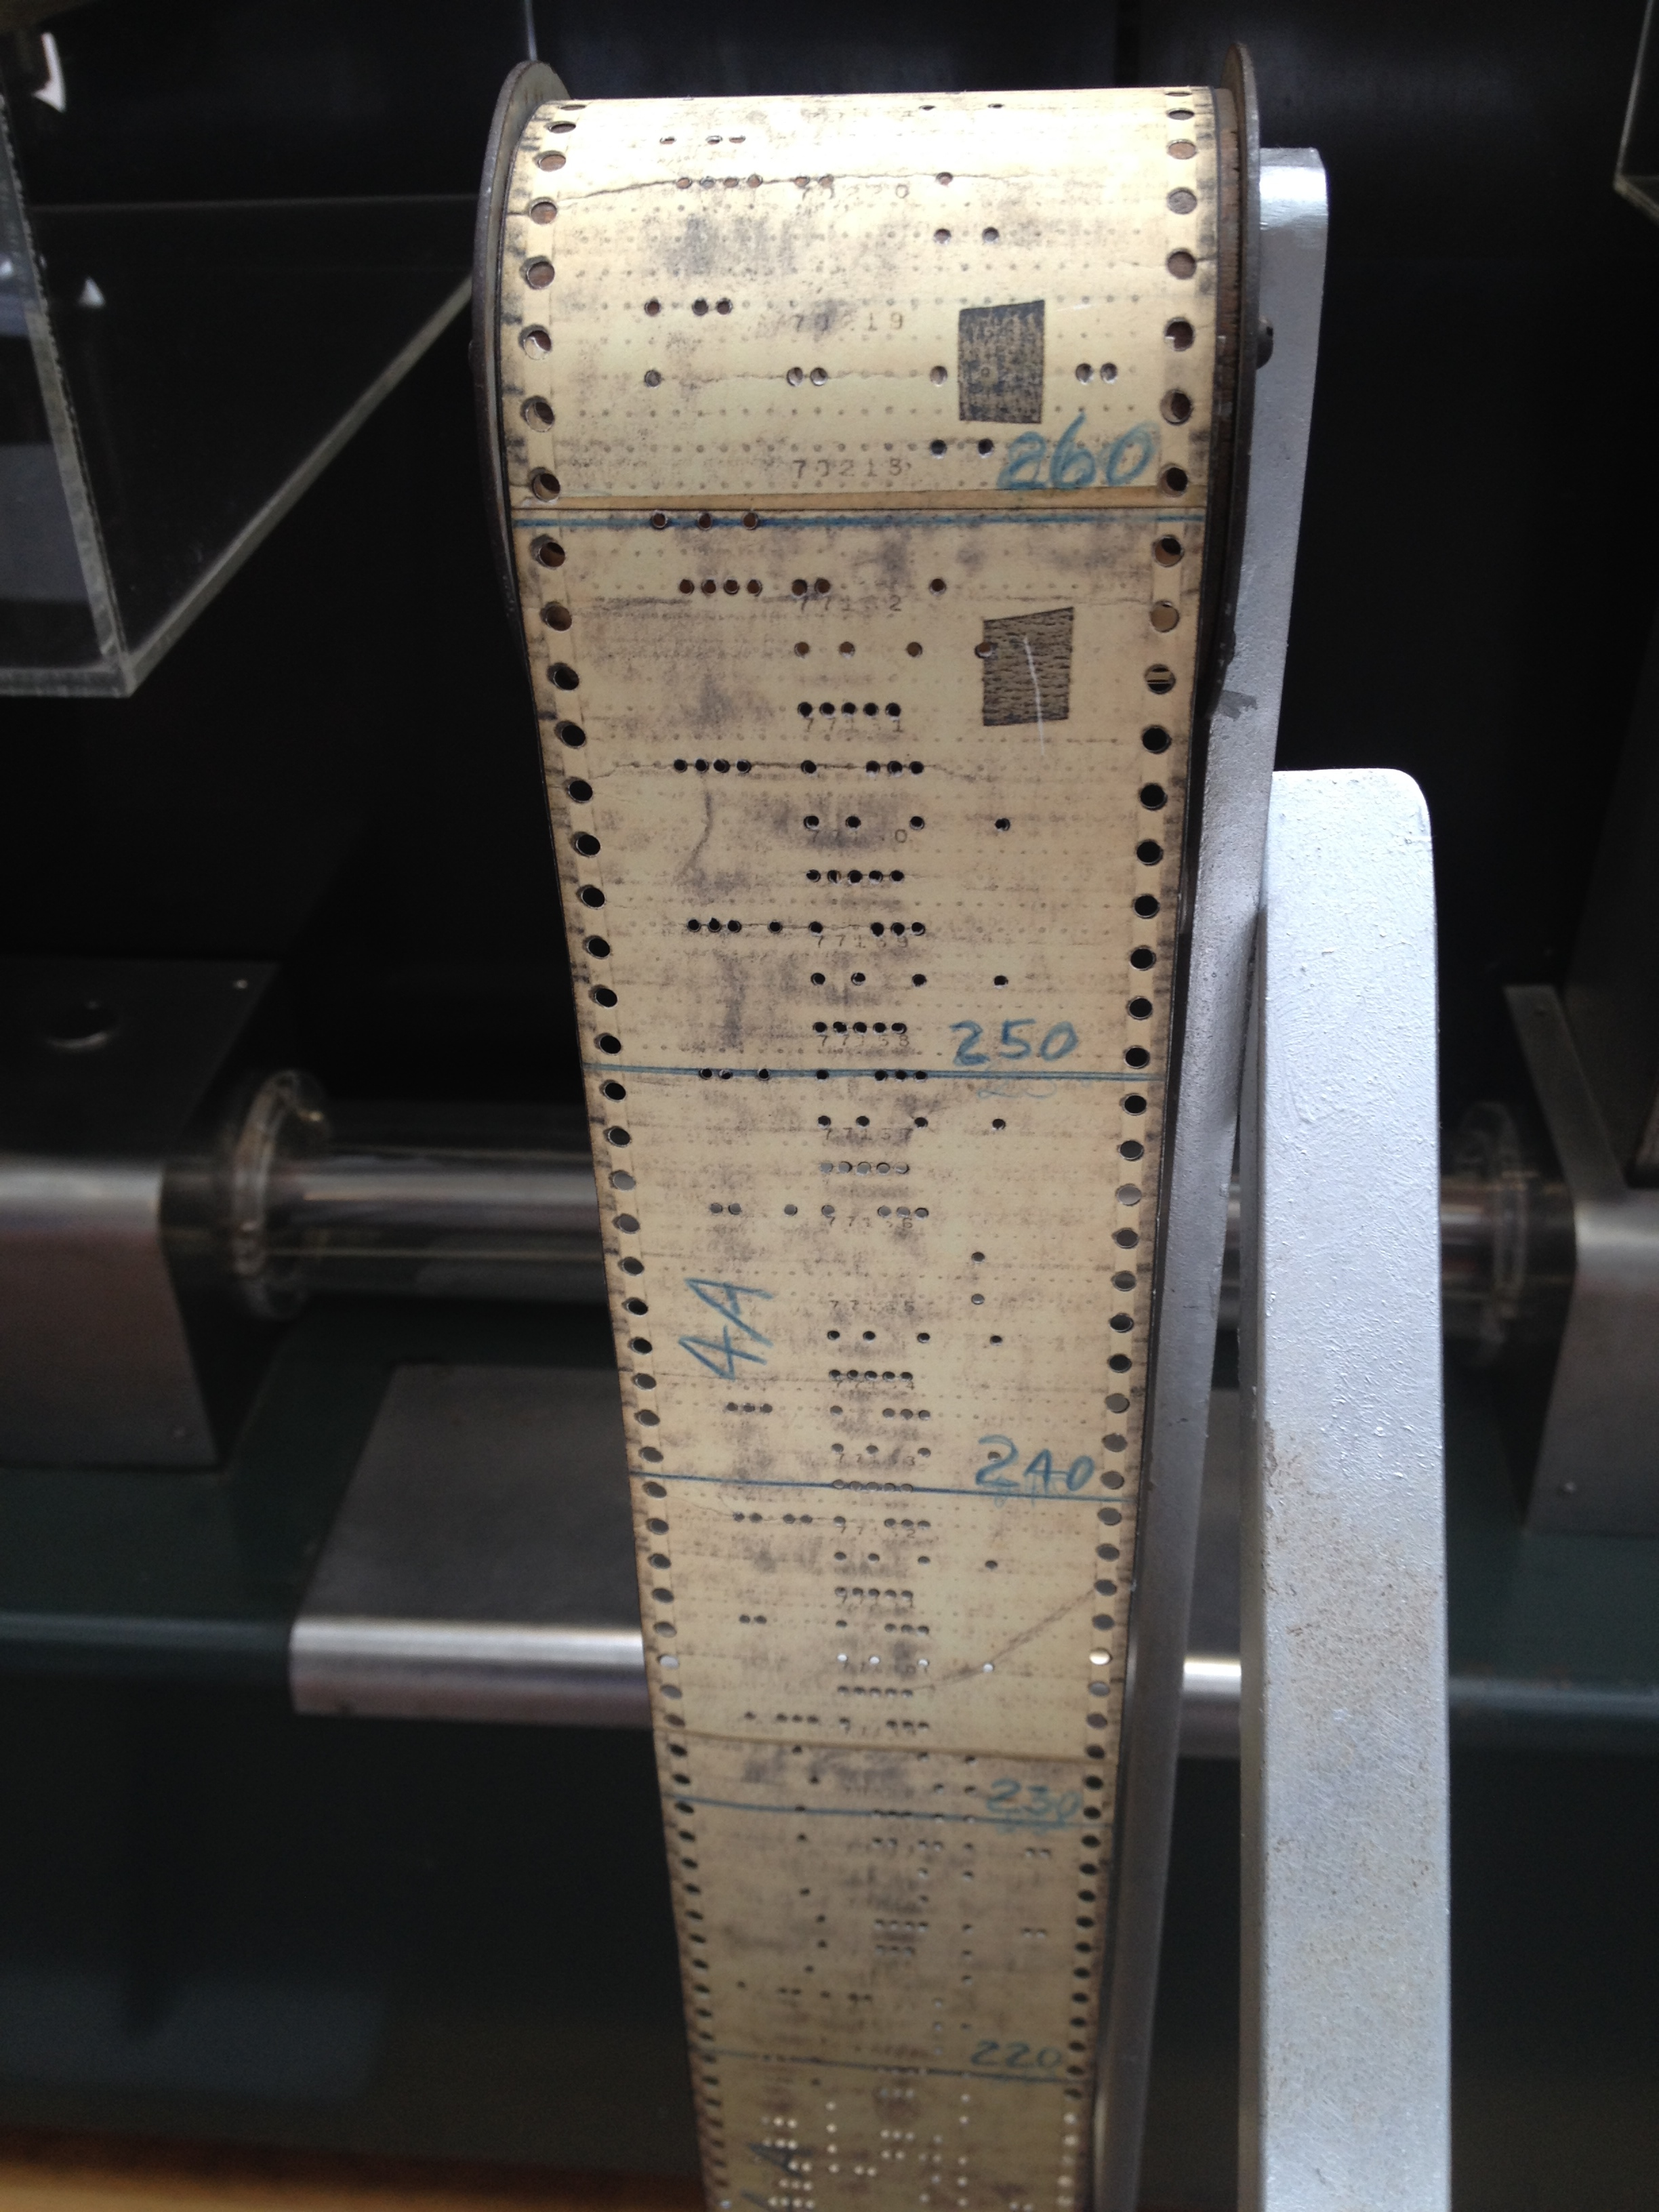
\includegraphics[scale=0.05]{./figures/C02-mark_i_instruction_tape}
  \captionsetup{justification=centering}
  \caption{Cinta de papel perforado con instrucciones de la Mark I}
  \label{fig:C02-mark_i_instruction_tape}
\end{figure}
La Mark I fue sucedida por la Mark II en el año 1948, la Mark III en septiembre de 1949 y la Mark IV en el año 1952, todos estos proyectos fueron de Aiken. La Mark II fue una mejora sobre la Mark I, pero aún basada en componentes electromecánicos. La tercer versión utilizaba en su mayoría componentes electrónicos tales como válvulas de vacío y diodos cristalinos, pero utilizaba cilindros magnéticos para almacenamiento, y relés para la transferencia de datos entre ellos. La cuarta versión fue la primera en ser completamente electrónica, reemplazando los cilindros magnéticos de almacenamiento con memorias de núcle magnético; el tipo de memoria de acceso aleatorio predominante entre 1955 y 1975.

\subsubsection{Harvard vs. von Neumann y Harvard modificada}

Como fue establecido al principio de esta sección, lo que diferencia estas dos arquitecturas es el acceso a los datos y a las instrucciones. La arquitectura von Neumann puede tratar a los datos como instrucciones y viceversa, dado que para dicha arquitectura, la memoria es exactamente la misma, con el mismo tipo de acceso y el mismo direccionamiento, contrariamente a lo que es una arquitectura puramente Harvard, cuyas memorias de datos e instrucciones se acceden por diferentes medios y cuyas direcciones pueden estar sobrepuestas (es decir que la misma dirección de memoria no representa lo mismo si se trata de datos o intrucciones) y por lo tanto, los datos y las intrucciones no pueden ser intercambiados en el tratamiento que se realiza dentro de la unidad de cómputo. Dadas estas condiciones, las principales desventajas son que, la arquitectura von Neumann no puede acceder simultáneamente a datos y a instrucciones y la máquina de Harvard no puede ni leer ni escribir en el espacio de memoria de las instrucciones, denegando por lo tanto cualquier posibilidad de código auto-optimizable o inteligente que reescriba sus instrucciones, así como tambíen la carga de los programas a partir de medios de almacenamiento de datos.\\
Hoy en día, las máquinas puramente Harvard no son más que una especialidad. Típicamente, en las máquinas modernas, se implementas arquitecturas Harvard modificadas. Estas modificaciones pueden ser de diversos tipos:

\subsection{Clasificación de las arquitecturas según su conjunto de instrucciones}

RISC vs CISC

La ISA define el modelo lógico: Tres cosas, los registros, el modelo de la memoria y como se relacionan los registros (operaciones).

\subsection{Taxonomía de Flynn}

Instruction and data streams


IMPORTANTE:

El modelo formal del procesador queda definida por el ISA. El isa no es una tabla de instrucciones. Es el modelo lógico formal que describe la arquitectura.

Hablar de Alan Turing. Problemas Turing Computables -> Investigar. Teorema de incompletitud de Gödel.	



% \chapter{Teoría de los sistemas MIMO}
% 
% En términos generales, se puede definir a un sistema MIMO (multiple input multiple output) como un sistema caracterizado por poseer múltiples entradas y salidas. Debido a la abstracción de esta definición, la misma puede ajustarse a distintos campos de estudio. El tema que se abordará será el estudio de sistemas MIMO en las radiocomunicaciones, en las cuales se trabajará con señales que provienen de ondas electromagnéticas. 
% 
% En este caso particular de comunicaciones, los sistemas MIMO se refieren a sistemas que poseen múltiples antenas para captar señales en la entrada y múltiples antenas para transmitir las señales de salida.
% 
% \begin{figure}[htb!]
%         \centering
%         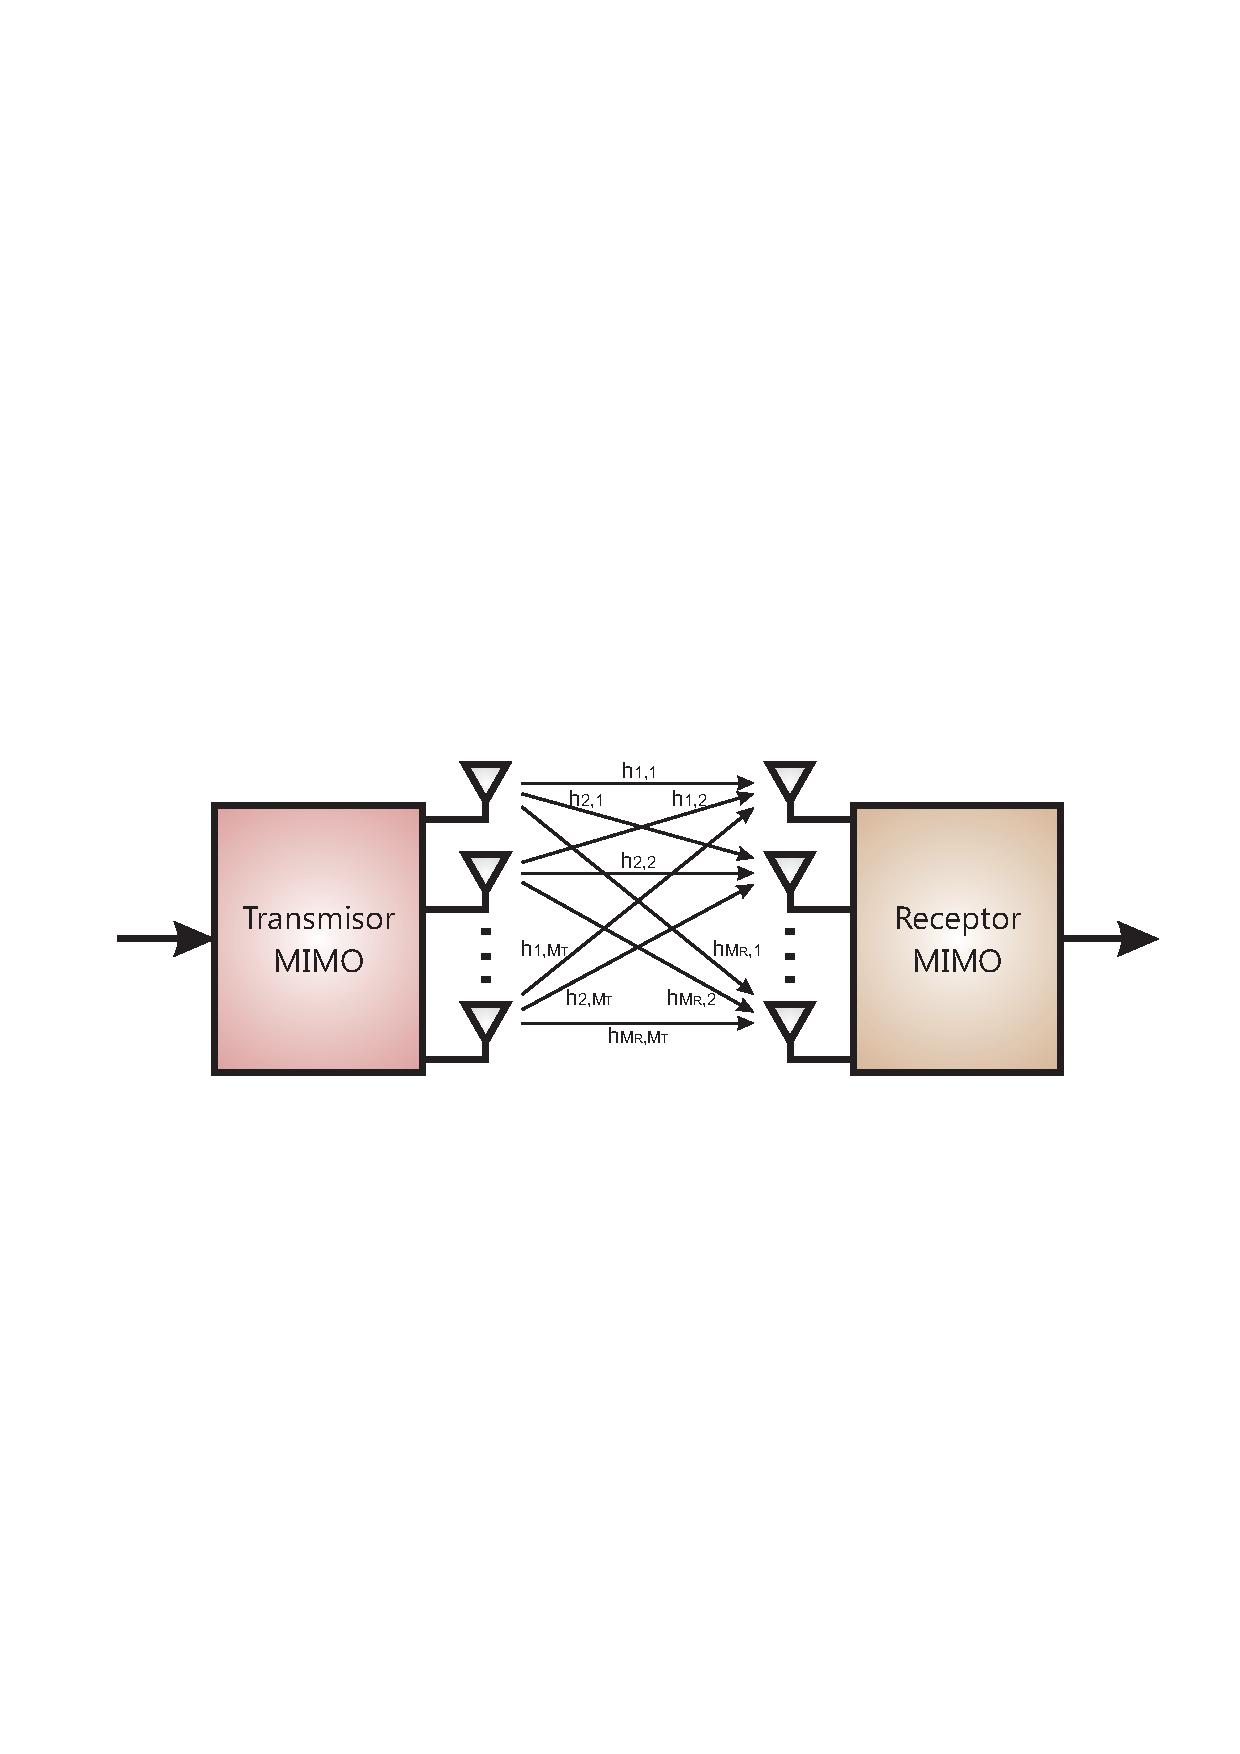
\includegraphics[width=11cm]{./figures/C02-MIMO_diagram_01}
%         \caption{Esquema de un sistema de comunicación MIMO}
%         \label{fig:MIMO_diagram_01}
% \end{figure}
% 
% Una comunicación inalámbrica se compone por tres elementos. Un transmisor, un receptor, y el canal, en el cual se propagan las señales a transmitir/recibir \cite{Mohammadi}. Existe una clasificación para los distintos tipos de sistemas MIMO en función de la cantidad de antenas que poseen en los lados emisor y receptor. MIMO propiamente dicho, se refiere a un sistema en el cual se tiene más de una única antena tanto en el receptor como en el emisor del sistema. Los sistemas en los cuales se tiene una única antena en el receptor y múltiples antenas en el transmisor son conocidos como MISO (multiple input single output). Por otro lado, los sistemas SIMO (single input multiple output), son aquellos en los cuales se tiene una única antena en el lado emisor y múltiples antenas en el lado receptor. SISO (single input single output) es el caso en el cual se tiene una única antena tanto en la entrada como en la salida.
% 
% \begin{figure}[htb!]
%         \centering
%         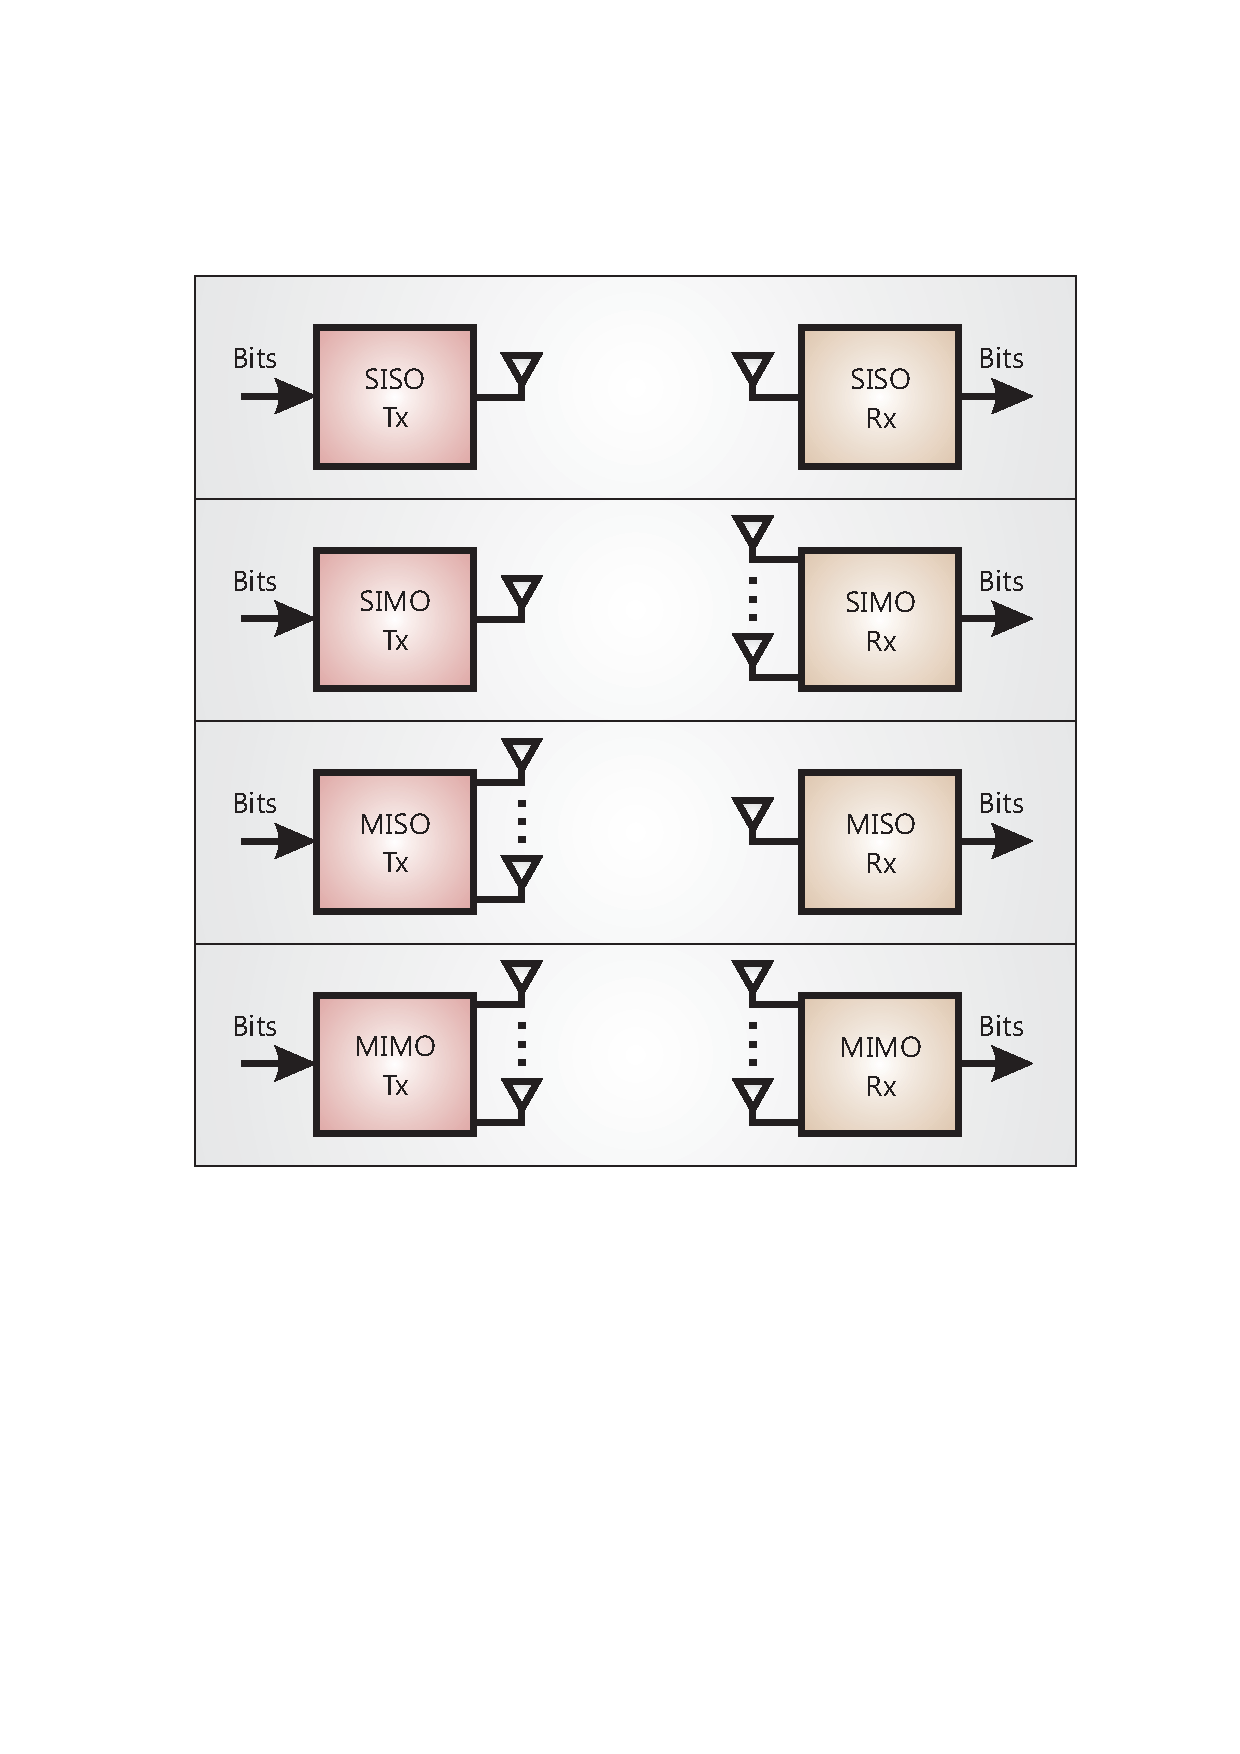
\includegraphics[width=8cm]{./figures/C02-MIMO_Combinations}
%         \caption{Representación de los distintos sistemas de múltiples antenas}
%         \label{fig:MIMO_Combinations}
% \end{figure}
% 
% El concepto de utilizar múltiples antenas en un receptor de comunicaciones inalámbricas surgió en 1960. La idea escencial consistía en la provisión de múltiples copias de una señal transmitida en el lado receptor y sus combinaciones para obtener una señal de mejor desempeño \cite{Mohammadi}. Ésta técnica, es conocida como \textbf{diversidad espacial}. Para lograr la técnica de diversidad espacial, se emplean múltiples antenas en el lado receptor. Las señales de las antenas de salida son luego combinadas aplicando distintos coeficientes de ponderación. Por otro lado, el estudio de la implementación de diversidad a través de múltiples antenas en el lado transmisor fue introducido en 1990 \cite{Paulraj}. 
% 
% A través de la utilización de múltiples antenas es posible lograr una mayor eficiencia en distintas características de un sistema de comunicación, siendo las más importantes el aumento en la capacidad del canal o en la relación señal ruido. También es posible resolver conflictos vinculados a distintos fenómenos asociados con una comunicación inalámbrica. Uno de estos fenómenos es el conocido como \textbf{\textit{``Multipath Fading''}}. Antes de abordar dicho fenómeno se hará una breve reseña de algunos conceptos sobre antenas.
% 
% \section{Antenas}
% 
% Una antena es un dispositivo eléctrico que convierte potencia eléctrica en ondas de radio, y viceversa. Usualmente, es utilizada con un radio transmisor o radio receptor. En una transmisión, el transmisor de radio provee una corriente eléctrica oscilante de radio frecuencia a las terminales de la antena, y la misma irradia la energía proveniente de dicha corriente como ondas electromagnéticas (ondas de radio). En la recepción, una antena intercepta parte de la potencia de una onda electromagnética con el objetivo de producir un voltaje muy pequeño en sus terminales, el cual es aplicado al receptor para luego ser amplificado \cite{Wiki_Antenna}.
% 
% La antena consiste de conductores eléctricos (cables, tubos o superficies reflectantes) que crean campos eléctricos y magnéticos en el espacio alrededor de los mismos. \cite{Haynes}. Si los campos son variantes, se propagan hacia el espacio como ondas electromagnéticas a la velocidad de la luz:
% 
% \begin{equation}
% \text{Velocidad de la Luz} \qquad  c \approx 3 \cdot 10^8 \frac{metros}{seg}
% \end{equation}
% 
% Toda antena que transmite también recibe. Las ondas electromagnéticas que atraviesan la misma excitan corrientes en los conductores de la antena. La antena captura parte de la energía de las ondas que la atraviesan y la convierte en señales eléctricas en el cable.
% 
% Al realizarse el diseño de una antena, sus dimensiones son especificadas en términos de la longitud de onda de las señales de radio que serán transmitidas o recibidas. La longiud de onda es la distancia desde el inicio de un ciclo electromagnético hasta el próximo.
% 
% \begin{equation}
% \lambda = \frac{c}{f_c}
% \end{equation}
% 
% $\lambda$ es la longitud de onda en metros y $f_c$ es la frecuencia portadora de señal de radio en $Hz$. c es la velocidad de la luz ($3 \cdot 10^8 metros/seg$).
% 
% 
% \begin{table}[htb!]
%     \begin{center}
%         \begin{tabular}{|c|c|c|}
%         \hline  
%         \textbf{Señal} & \textbf{Frecuencia} & \textbf{Longitud de Onda} \\
%         \hline  
%         Radio AM & $1 MHz$ & 300 metros \\
%         \hline
%         Radio FM & $100 MHz$ & 3 metros \\
%         \hline
%         Teléfono Celular & $850 MHz$ & 35 centímetros \\
%         \hline
%         Access Point Wi-Fi & $2,4 GHz$ & 12,5 centímetros \\
%         \hline
%         \end{tabular}
%         \caption{Ejemplos de bandas de frecuencias y sus longitudes de onda}
%     \end{center}
% \end{table}
% 
% 
% \subsection{Patrón de radiación de una antena}
% 
% Una antena transmisora genera ondas electromagnéticas más fuertes en algunas direcciones con respecto a otras. Para analizar este comportamiento se obtiene un diagrama de intensidad del campo en función de la dirección, el cual es llamado ``Patrón de radiación de la antena''. Siempre es igual para la recepción y para la transmisión.
% 
% Una onda electromagnética medida en un punto lejos de la antena es la suma de la radiación de todas las partes de la antena. Cada parte de la misma, irradia ondas de diferentes amplitudes y fases, y cada una de esos ondas viaja distintas distancias hasta el punto donde se encuentra el receptor. En algunas direcciones, estas ondas se suman constructivamente para dar una ganancia. En otras, se suman destructivamente para dar una pérdida.
% 
% Un dipolo de media onda es una antena simple que consiste de media longitud de onda de cable, cortado en el centro para realizar la conexión. En la siguiente figura se muestra su patrón de radiación:
% 
% \begin{figure}[htb!]
%         \centering
%         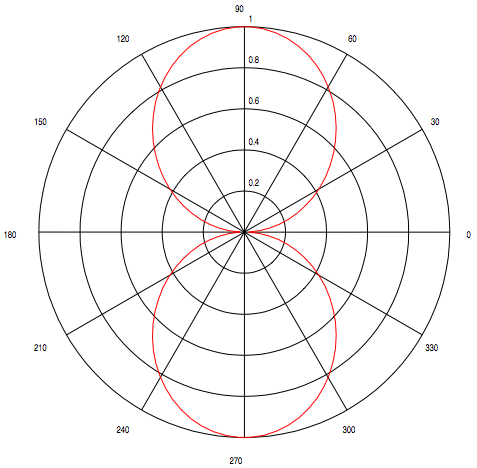
\includegraphics[width=6cm]{./figures/C02-half_wave_dipole}
%         \caption{Dipolo de media onda - Intensidad de Campo vs Dirección}
%         \label{fig:half_wave_dipole}
% \end{figure}
% 
% \begin{figure}[htb!]
%         \centering
%         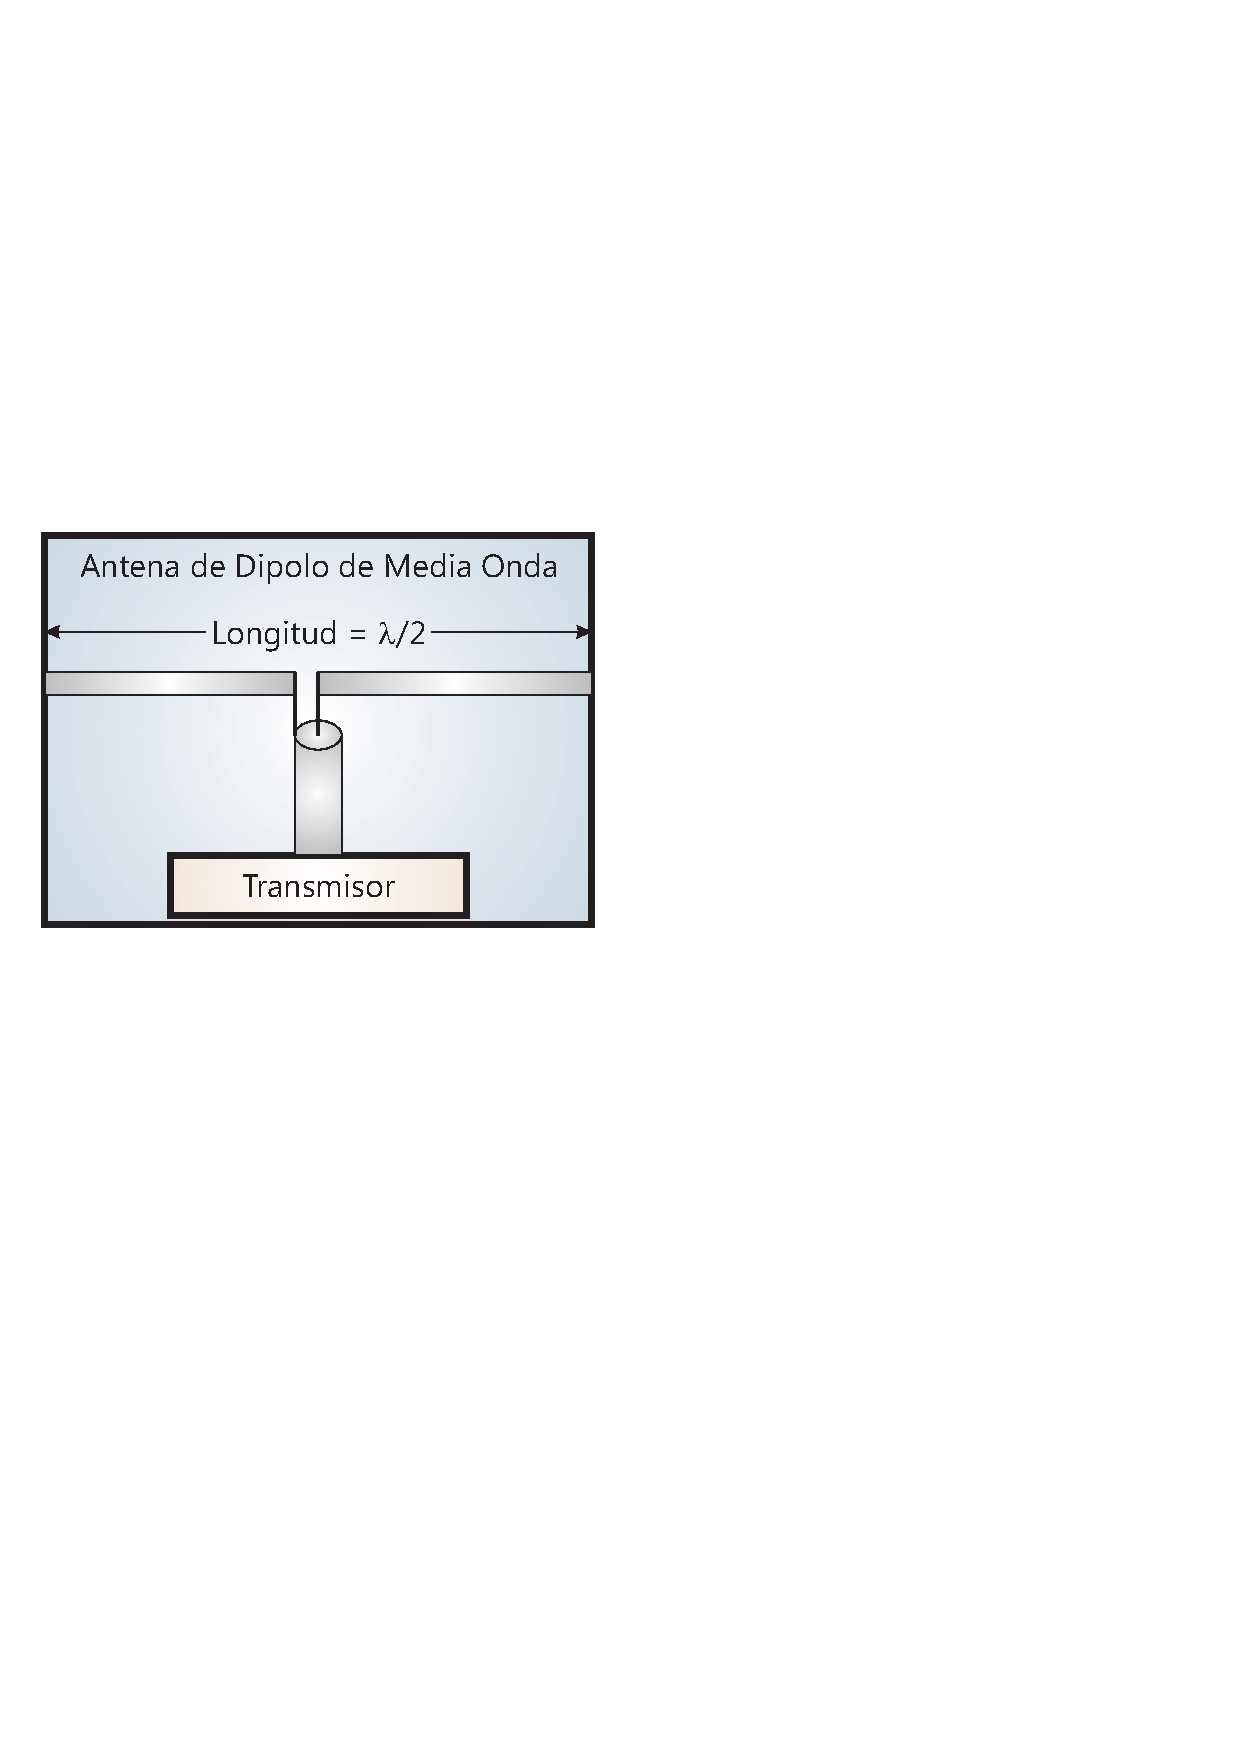
\includegraphics[width=6cm]{./figures/C02-half_wave_dipole_2}
%         \caption{Dipolo de media onda - Esquema}
%         \label{fig:half_wave_dipole_2}
% \end{figure}
% 
% \subsection{Antenas direccionales}
% 
% Un ejemplo de antena direccional es una antena diseñada para tener ganancia en una dirección y pérdida en otras. Una antena se vuelve direccional al aumentar su tamaño. Al hacer esto, se amplian los conductores radiantes de la antena para cubrir una distancia mayor, de forma tal que las interferencias constructivas y destructivas pueden ser controladas de mejor forma para dar un patrón de radiación direccional.
% 
% Una antena de plato satelital puede ser considerada, simplisticamente, una superficie circular que irradia ondas electromagnéticas igualmente desde todas partes. Tiene un haz central angosto de alta ganancia, como se muestra en la siguiente figura, que se apunta al satélite.
% 
% A medida que se incrementa el diametro del plato en longitudes de onda, el haz central se vuelve más angosto. Notar los lóbulos pequeños, llamados ``lóbulos laterales'', a cada lado del haz central. Las direcciones en las cuales la intensidad de señal es cero son llamadas `nulls''.
% 
% \begin{figure}[htb!]
%         \centering
%         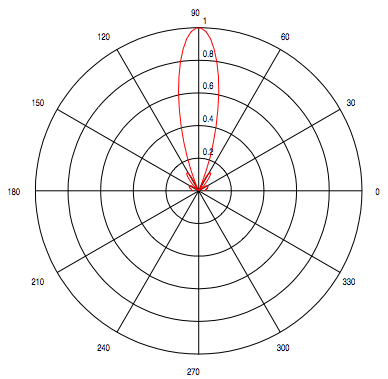
\includegraphics[width=6cm]{./figures/C02-dish_antenna}
%         \caption{Antena Parabólica - Patrón de Radiación}
%         \label{fig:dish_antenna}
% \end{figure}
% 
% \begin{figure}[htb!]
%         \centering
%         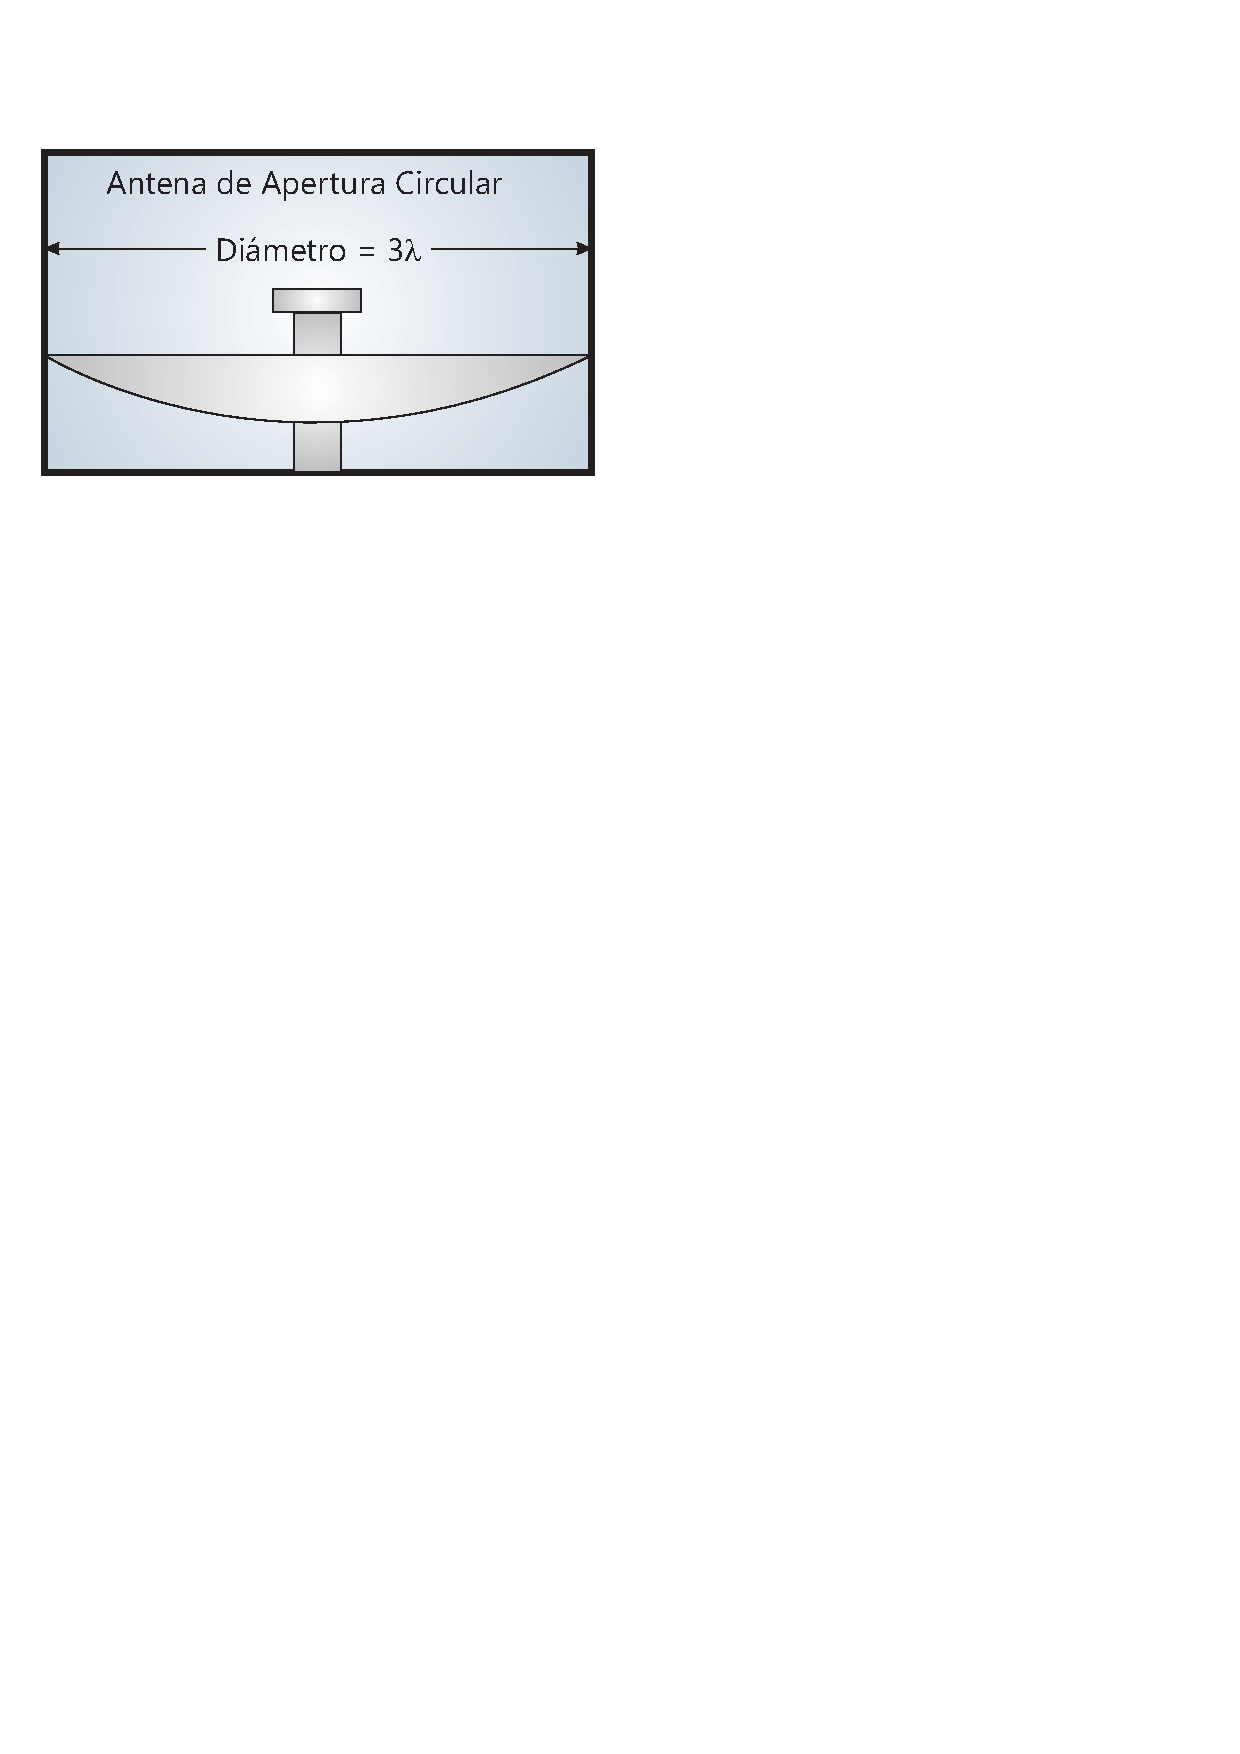
\includegraphics[width=6cm]{./figures/C02-dish_antenna_2}
%         \caption{Antena Parabólica - Diagrama}
%         \label{fig:dish_antenna_2}
% \end{figure}
% 
% \subsection{Arreglos lineales}
% 
% Una antena direccional simple consiste de un arreglo lineal de pequeños elementos radiantes de antena, cada uno alimentado con señales idénticas (misma amplitud y fase) desde un transmisor. A medida que el ancho total del arreglo crece, el haz central se vuelve más angosto. A medida que el número de elementos se incrementa, los lóbulos laterales se vuelven más pequeños.
% 
% La siguiente figura es el patrón de raciación para una linea de 4 elementos (antenas pequeñas) espaciadas $1/2$ longitud de onda.
% 
% \begin{figure}[htb!]
%         \centering
%         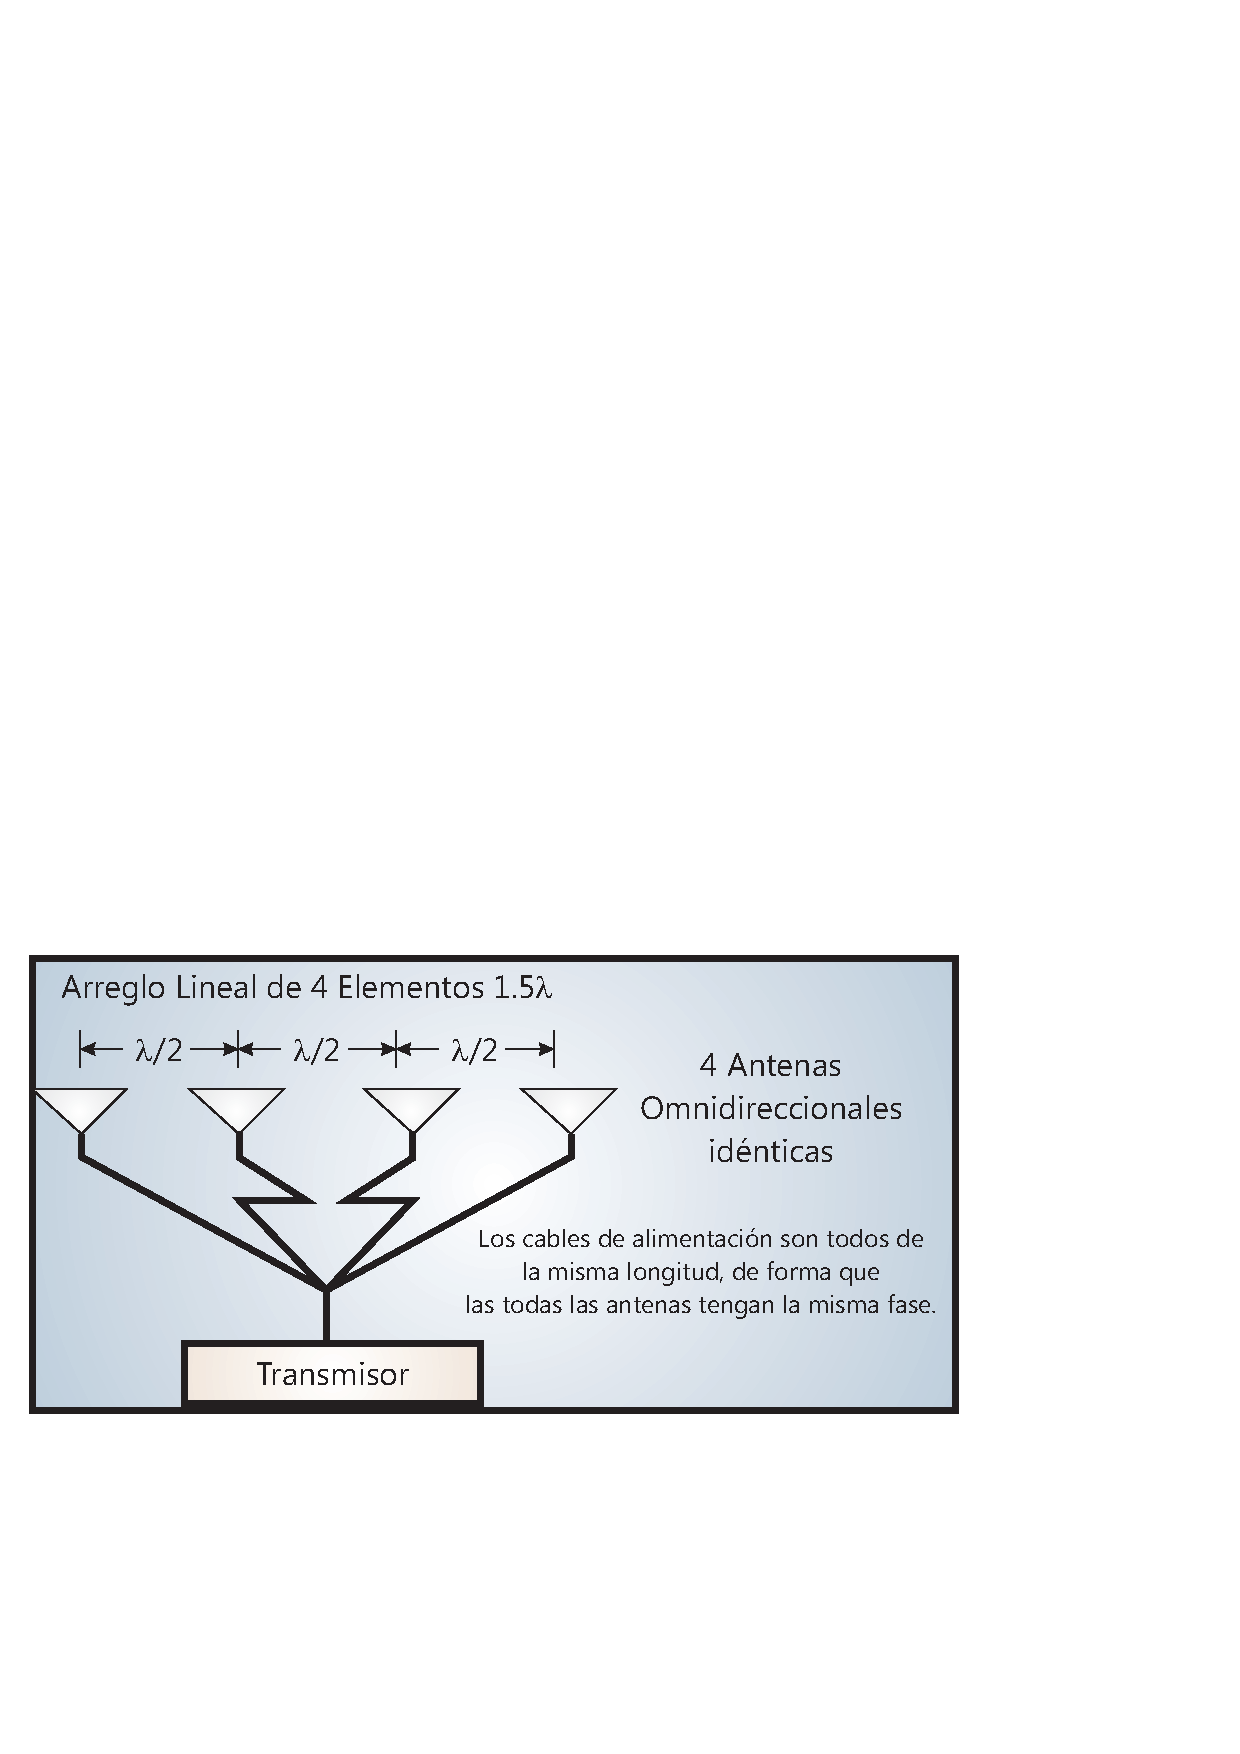
\includegraphics[width=7cm]{./figures/C02-linear_array_1}
%         \caption{Arreglo Lineal $D=\lambda/2$ - Patrón de Radiación}
%         \label{fig:linear_array_1}
% \end{figure}
% 
% \begin{figure}[htb!]
%         \centering
%         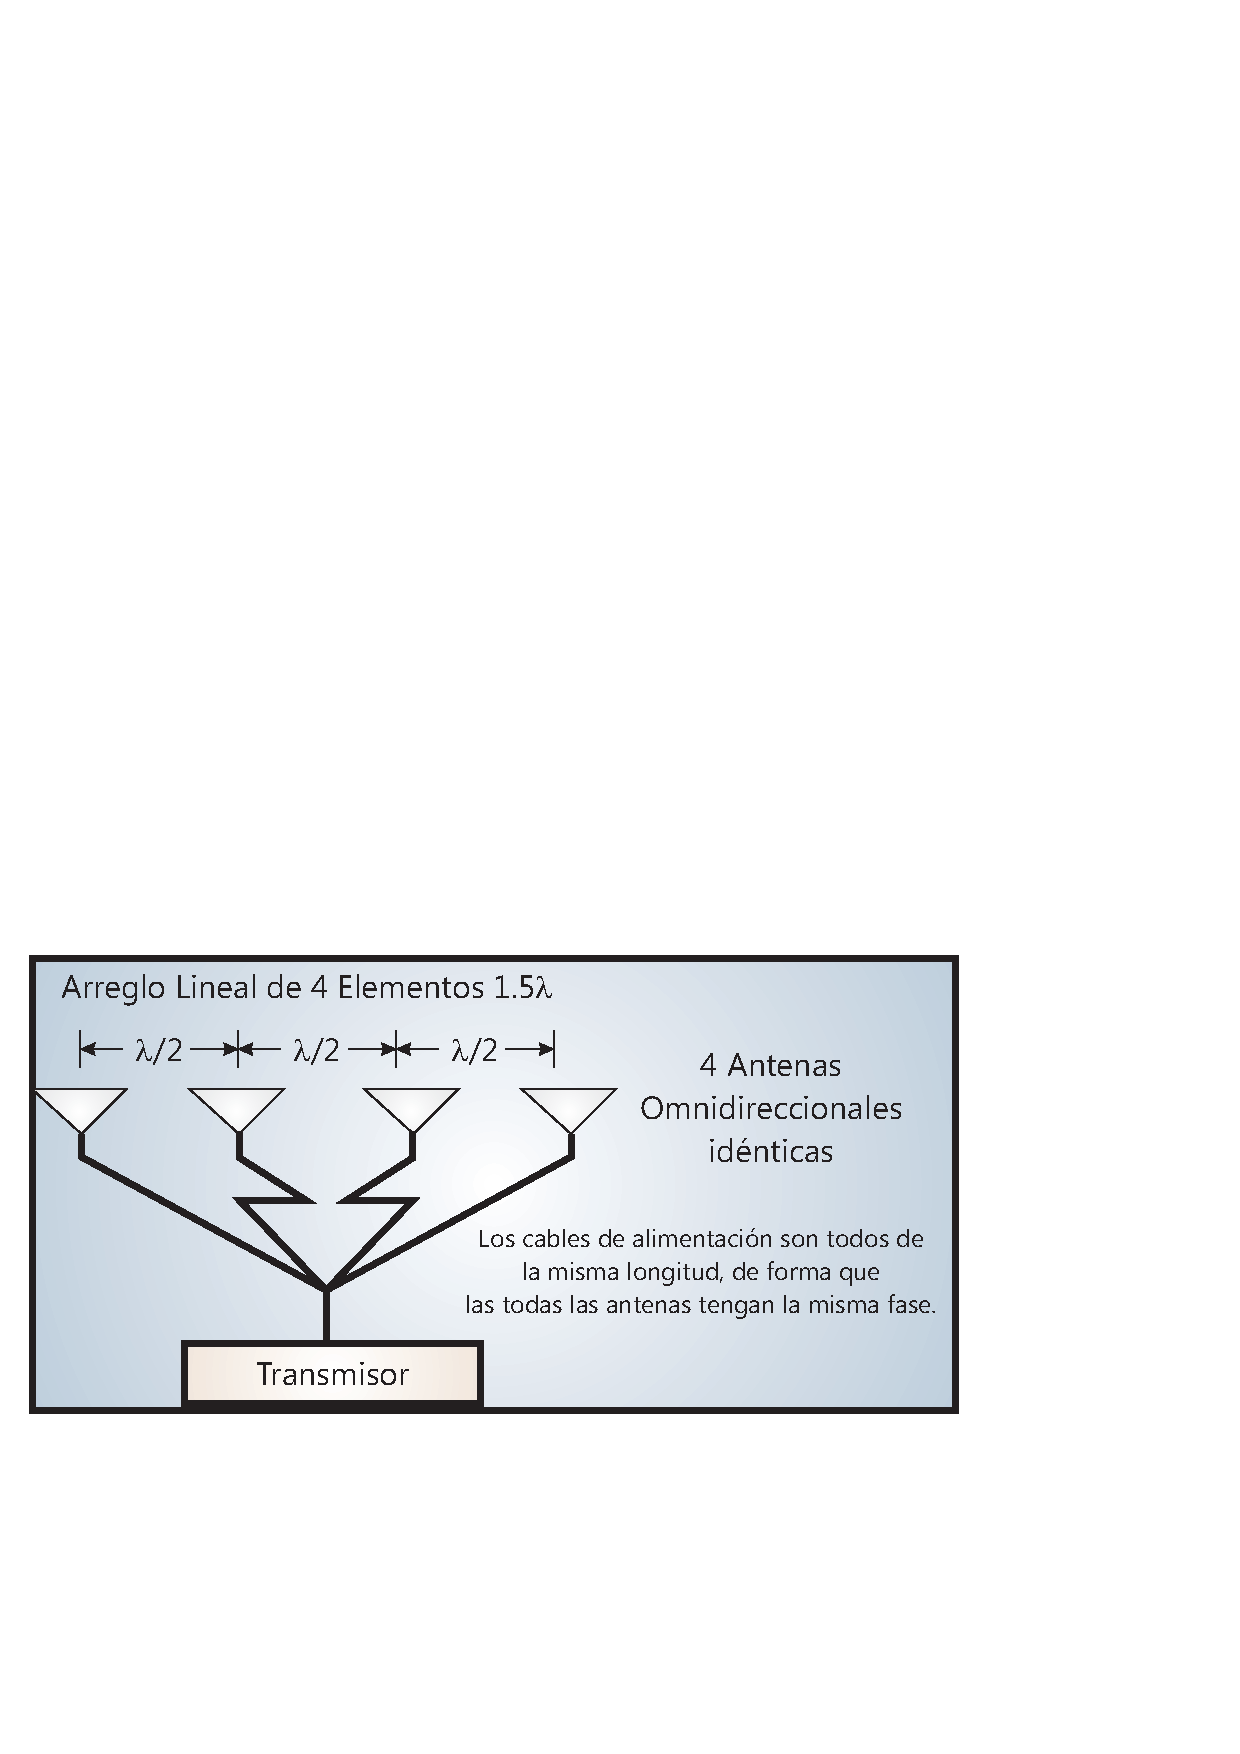
\includegraphics[width=9cm]{./figures/C02-linear_array_1_b}
%         \caption{Arreglo Lineal $D=\lambda/2$ - Esquema}
%         \label{fig:linear_array_1_b}
% \end{figure}
% 
% Si el espaciado es incrementado a más de $1/2$ longitud de onda, empiezan a aparecer lóbulos laterales más largos en el patrón de radiación. De todas formas, el haz central se vuelve más angosto debido a que la longitud total de la antena es incrementada. A continuación se ilustra el siguiente patrón de radiación, para 4 elementos espaciados $1$ longitud de onda:
% 
% \begin{figure}[htb!]
%         \centering
%         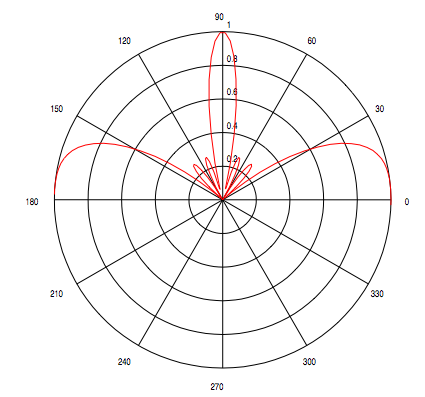
\includegraphics[width=6cm]{./figures/C02-linear_array_2}
%         \caption{Arreglo Lineal $D=\lambda$ - Patrón de Radiación}
%         \label{fig:linear_array_2}
% \end{figure}
% 
% Al mantener la longitud total de la antena igual, y agregar elementos para reducir el espaciado nuevamente a $1/2$ longitud de onda, los lóbulos laterales se reducen. A continuación se muestra el patrón de radiación si se agregan 3 elementos más a la antena anterior para reducir el espaciado entre elementos.
% 
% \begin{figure}[htb!]
%         \centering
%         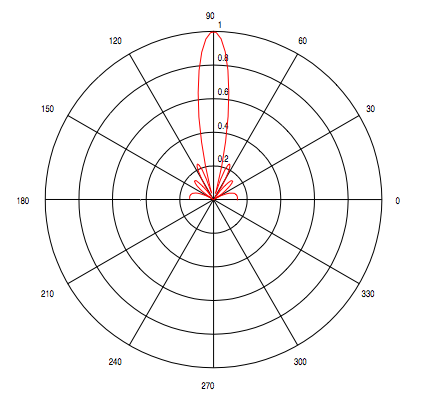
\includegraphics[width=6cm]{./figures/C02-linear_array_3}
%         \caption{Arreglo Lineal $D=\lambda/2$ - 7 elementos - Patrón de Radiación}
%         \label{fig:linear_array_3}
% \end{figure}
% 
% \begin{figure}[htb!]
%         \centering
%         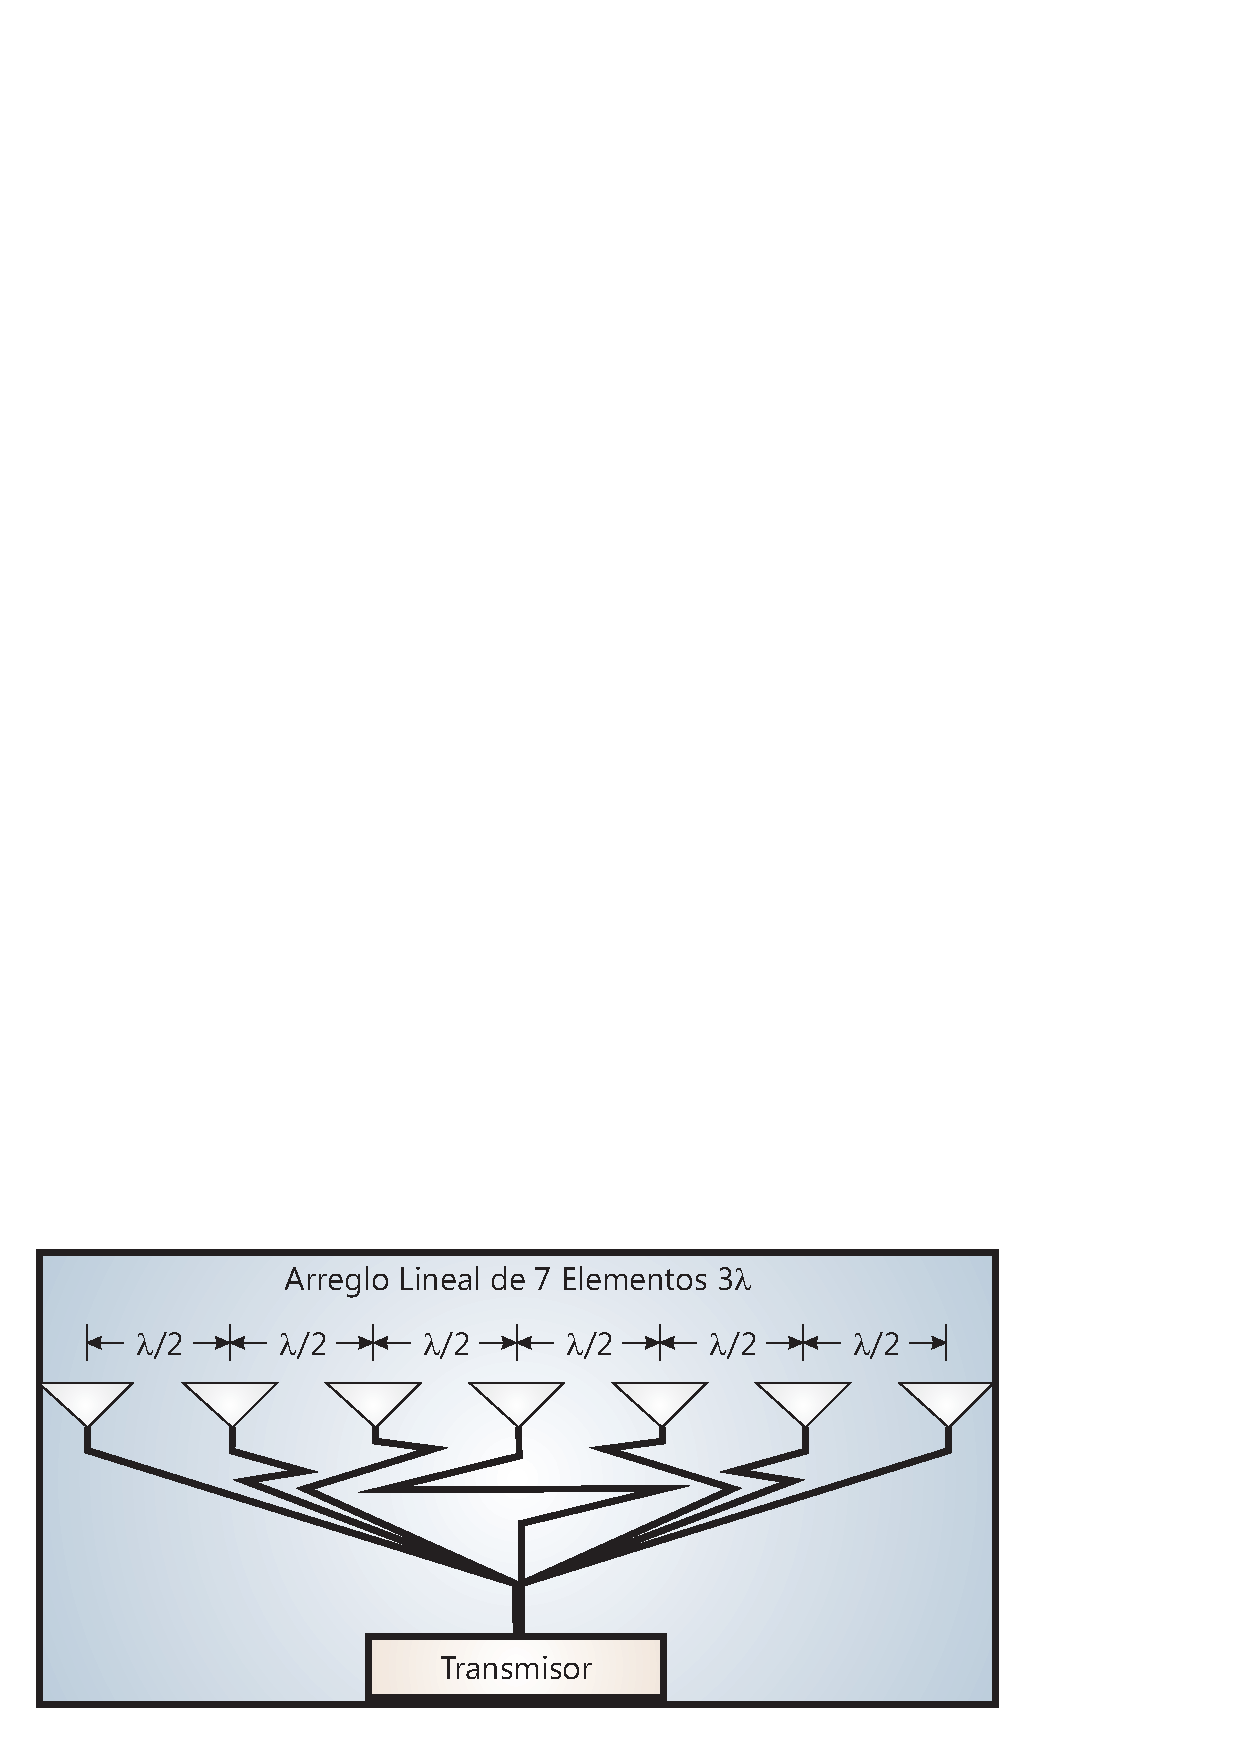
\includegraphics[width=10cm]{./figures/C02-linear_array_4}
%         \caption{Arreglo Lineal $D=\lambda/2$ - 7 elementos - Esquema}
%         \label{fig:linear_array_4}
% \end{figure}
% 
% \subsection{Arreglos dirigidos electrónicamente}
% 
% El haz central del arreglo lineal puede ser direccionado al variar las fases de las señales en los elementos del mismo. La forma más simple para controlar la fase de las señales es variar sistemáticamente las longitudes de los cables hacia los elementos. El cable retrasa la señal, por lo cual desplaza la fase. De todas formas, esto no permite que la antena sea dirigida dinámicamente.
% 
% En un arreglo electrónicamente dirigido, se utilizan desplazadores de fase electrónicos programados en cada elemento del arreglo. La antena es dirigida al programar el valor de desplazamiento de fase requerido para cada elemento. El patrón del haz a continuación es para un arreglo lineal de 8 elementos con un desplazamiento de fase progresivo de $0,7 \pi$ por elemento. El haz central fue dirigido 45 grados a la izquierda. Un desplazamiento de fase de $2 \pi$ corresponde a una longitud de onda o un periodo de onda de portadora, y valores más positivos son equivalentes a decir que la señal es transmitida más tempranamente.
% 
% \begin{figure}[htb!]
%         \centering
%         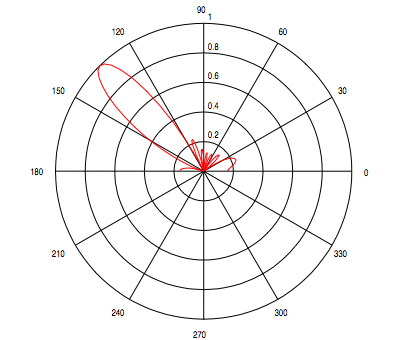
\includegraphics[width=6cm]{./figures/C02-steered_array}
%         \caption{Arreglo dirigido electrónicamente - Patrón de Radiación}
%         \label{fig:steered_array}
% \end{figure}
% 
% \begin{figure}[htb!]
%         \centering
%         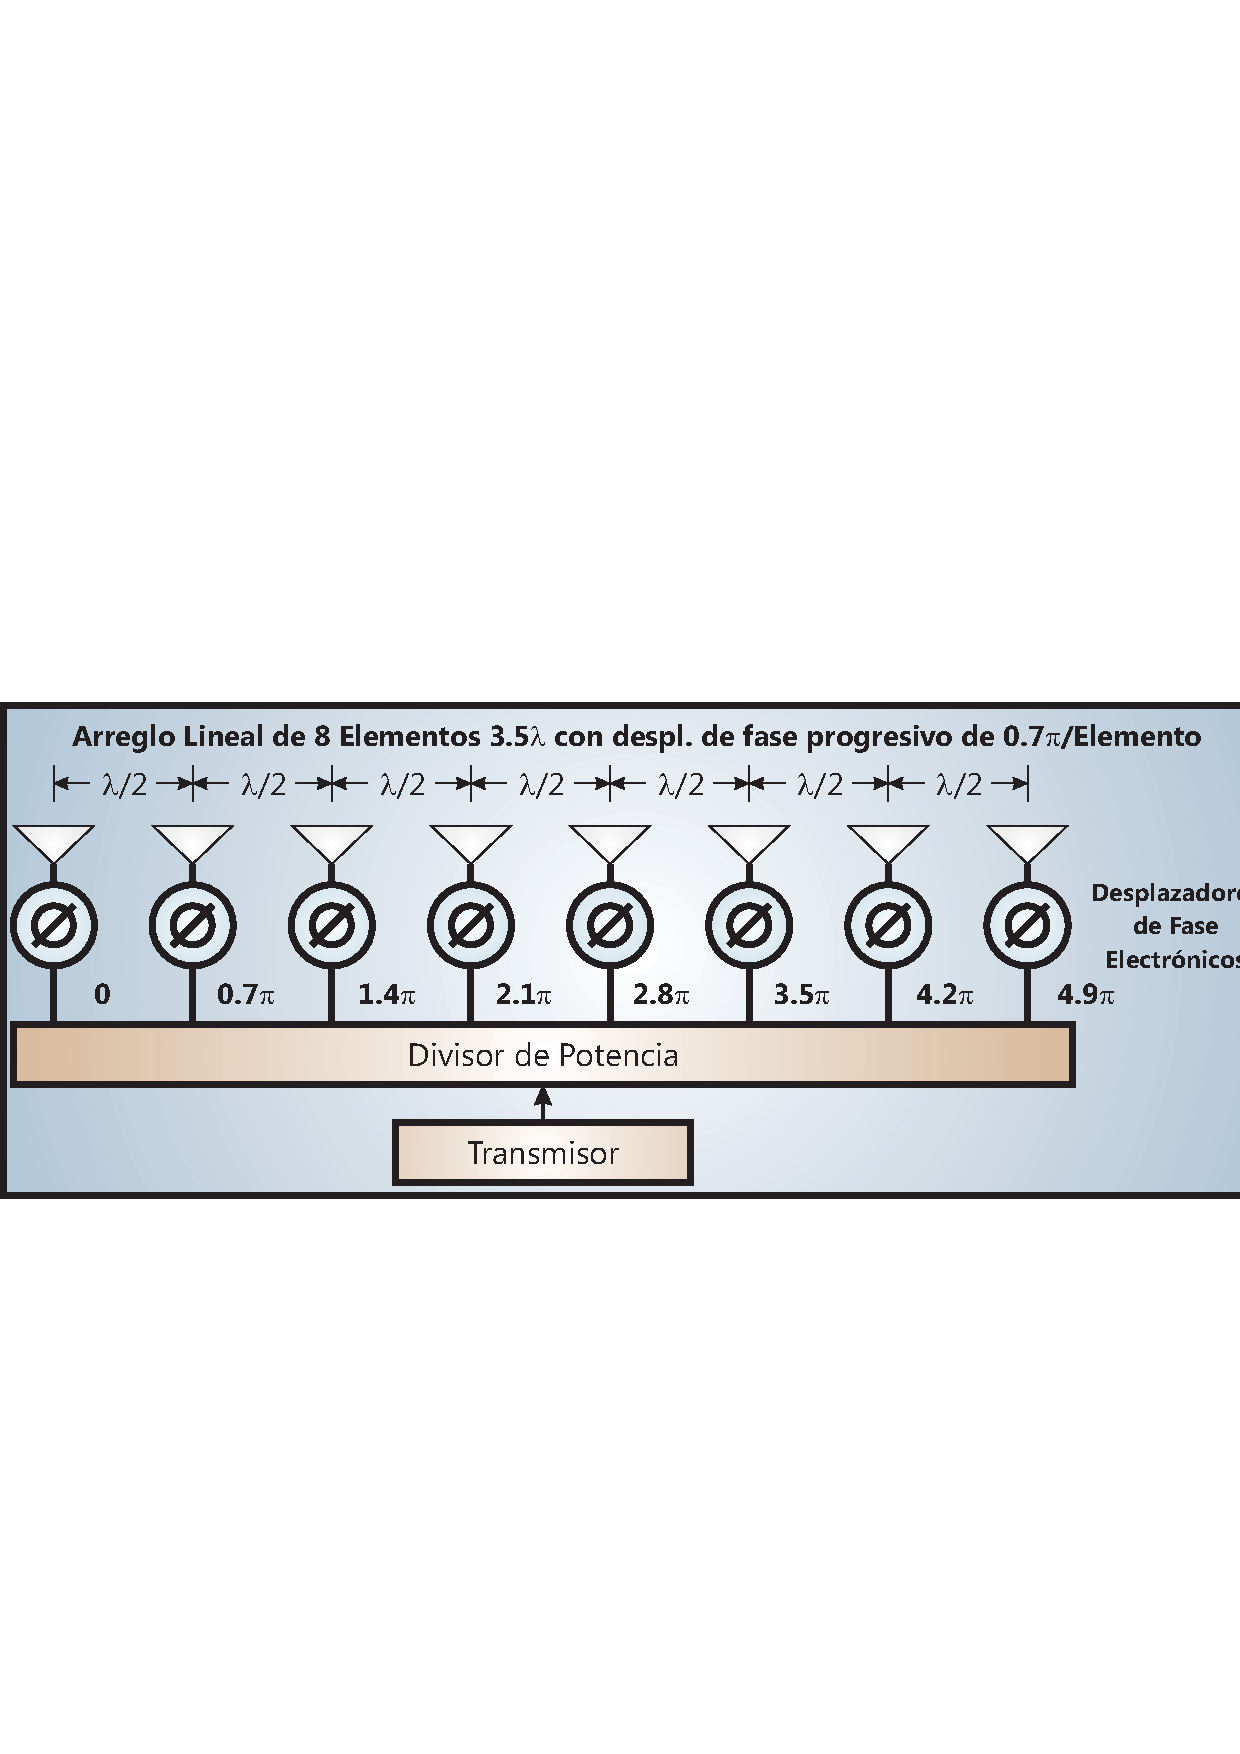
\includegraphics[width=11cm]{./figures/C02-steered_array_2}
%         \caption{Arreglo dirigido electrónicamente - Esquema}
%         \label{fig:steered_array2}
% \end{figure}
% 
% \subsection{Parámetros básicos de arreglos de antenas}
% 
% A continuación se explicarán algunos parámetros y definiciones básicas que serán de interés relevante para los conceptos tratados en la presente tesis \cite{Litva}. A pesar de que varios de ellos son definidos en términos de antenas transmisoras, la reciprocidad asegura que estas definiciones sean también aplicables a antenas receptoras.
% 
% \subsubsection{Patrón de radiación}
% 
% Se refiere a la distribución relativa de potencia irradiada como función de la dirección en el espacio.
% 
% \subsubsection{Factor del arreglo}
% 
% El factor del arreglo representa el patrón de raciación a campo lejano de un arreglo isotrópico de elementos radiantes. El factor del arreglo se denotará a lo largo de la tesis como $F(\phi,\theta)$, donde $\phi$ representa el ángulo de azimuth y $\theta$ representa el ángulo de elevación en el espacio.
% 
% \subsubsection{Lóbulo principal}
% 
% El lóbulo principal de un patrón de radiación de una antena es el lóbulo que contiene la dirección de máxima radiación de potencia.
% 
% \subsubsection{Lóbulos laterales}
% 
% Los lóbulos laterales son lóbulos en cualquier dirección distinta de aquella del lóbulo principal. Para un arreglo lineal con ponderación uniforme, el primer lóbulo lateral (el cual es el más cercano al lóbulo principal) en el patrón de radiación se encuentra $13 dB$ por debajo del valor pico del lóbulo principal.
% 
% \subsubsection{Ancho del haz (Beamwidth)}
% 
% El ancho del haz de una antena es el ancho angular del lobulo principal en su patrón de radiación a campo lejano. El HPBW (Ancho del haz a mitad de potencia), o ancho del haz a $-3 dB$, es el ancho del haz medido entre los puntos del lóbulo principal que se encuentran a $-3 dB$ del valor pico del lóbulo principal:
% 
% \begin{equation}
% HPBW = \frac{0.88 \lambda}{A}
% \end{equation}
% 
% Donde $A$ representa la longitud de la apertura del arreglo.
% 
% \subsubsection{Eficiencia de la antena}
% 
% La eficiencia de la antena se define como la relación entre la potencia total irradiada por la antena y la potencia total de entrada de la misma.
% 
% \subsubsection{Ganancia directiva}
% 
% La ganancia directiva es una cantidad definida para campo lejano como la relación entre la densidad de radiación en una dirección angular particular en el espacio y la densidad de radiación de la misma potencia irradiada isotrópicamente, lo que es:
% 
% \begin{equation}
% D(\phi,\theta) = \frac{4 \pi \text{ potencia irradiada por unidad de ángulo sólido en dirección } \phi,\theta }{\text{Total de potencia irradiada por la antena}}
% \end{equation}
% 
% \subsubsection{Directividad}
% 
% La directividad es la máxima ganancia directiva de la antena, es decir, la ganancia directiva en la dirección de máxima densidad de radiación.
% 
% \subsubsection{Ganancia de la antena}
% 
% La ganancia de la antena es definida como la relación entre la densidad de radiación en una dirección particular del espacio y la potencia total de entrada de la antena:
% 
% \begin{equation}
% G(\phi,\theta) = \frac{4 \pi \text{ potencia irradiada por unidad de ángulo sólido en dirección } \phi,\theta }{\text{Total de potencia irradiada por la antena}}
% \end{equation}
% 
% La ganancia máxima G, o simplemente ganancia, es el producto entre la directividad y la eficiencia de la antena, es decir:
% 
% \begin{equation}
% G = D \eta
% \end{equation}
% 
% \section{\textit{Multipath fading}}
% 
% Cuando se transmite una señal a través de una antena, la misma se propaga en el medio y enfrenta distintos tipos de obstáculos, tales como el suelo, edificios, autos, personas e incluso las distintas capas de la atmósfera. Se producirán reflexiones y desfasajes que darán lugar a señales que provienen de distintos caminos o direcciones, las cuales se sumarán para obtener una señal resultante en la antena receptora. A este efecto se lo conoce como \textbf{\textit{Multipath Fading}} \cite{Pahlavan}.
% 
% \begin{figure}[htb!]
%         \centering
%         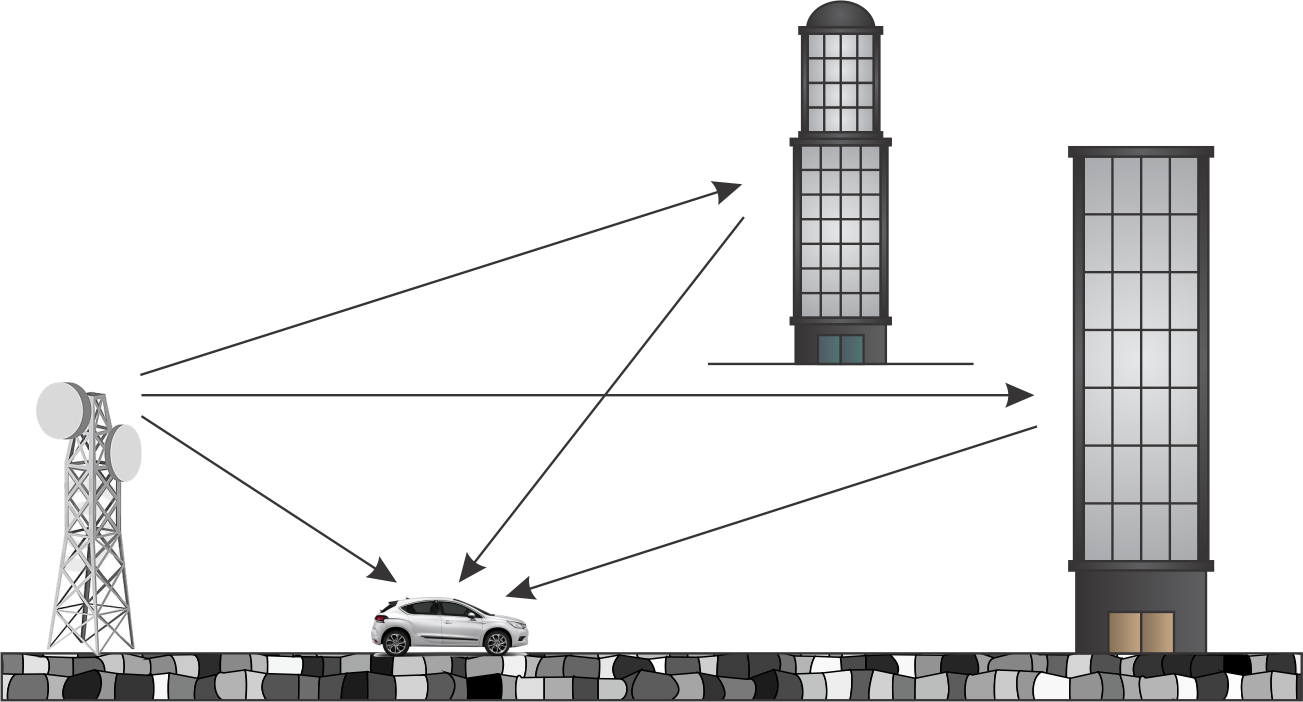
\includegraphics[width=10cm]{./figures/C02-multipath_fading}
%         \caption{Múltiples Reflexiones de la señal transmitida}
%         \label{fig:MultipathFading}
% \end{figure}
% 
% La presencia de reflectores en el ambiente que rodea al transmisor y receptor, crea múltiples caminos que la señal transmitida puede recorrer. La amplitud y la fase de la señal que llega desde cada camino estará relacionada con la longitud del camino y las condiciones, lo cual resulta en fluctuaciones considerables en la amplitud de la señal compuesta recibida. Esto puede resultar en una interferencia constructiva o destructiva, amplificando o atenuando la potencia de señal vista desde el receptor.
% 
% El análisis preciso de la propagación por múltiples caminos puede ser abordado a través del uso de las ecuaciones de Maxwell con condiciones de contorno que representen las propiedades físicas de la arquitectura y el medio ambiente. De todas formas, este análisis es muy complejo y se suele abordar el problema haciendo una derivación a las leyes de óptica geométrica, representando a la propagación de ondas electromagnéticas como la propagación de ondas ópticas.
% 
% Cuando se produce una interferencia destructiva de gran intensidad, se la reconoce como \textbf{\textit{deep fade}} y puede resultar en una falla temporal de la comunicación debido a una severa caída en la relación señal ruido del canal.
% 
% Por dichos motivos, es deseable encontrar una forma de poder abordar el fenómeno de \textit{multipath fading} con el objetivo de poder garantizar estabilidad y confiabilidad en la comunicación.
% 
% \section{\textit{Beamforming}}
% 
% \textit{Beamforming} consiste en la combinación de distinas señales de radio provenientes de un conjunto de antenas no direccionales, espacialmente separadas, con el objetivo de simular una gran antena direccional \cite{Haynes}. La antena simulada puede ser apuntada electrónicamente, a pesar de que físicamente, la antena no se mueva. En comunicaciones, la técnica de \textit{beamforming} es utilizada para apuntar una antena hacia la fuente de la señal para reducir la interferencia y mejorar la calidad de la comunicación. En aplicaciones de descubrimiento de dirección, \textit{beamforming} puede ser utilizado para dirigir una antena para determinar la dirección del origen de una señal.
% 
% \subsection{\textit{Beamforming} digital}
% 
% La técnica de \textit{beamforming} digital está basada en la conversión de una señal de RF proveniente de cada antena a dos flujos de señales binarias en banda base representando los canales I y Q \cite{Litva}. Las señales digitales en banda base luego representan las amplitudes y fases de las señales recibidas en cada elemento del arreglo. El proceso de \textit{beamforming} implica la ponderación de estas señales digitales, ajustando sus amplitudes y fases de forma tal que al ser sumadas en conjunto formen el haz deseado. Básicamente, un sistema de \textit{beamforming} digital consta de un arreglo de antenas, receptores individuales para cada una de ellas, y un procesador digital de señales.
% 
% \begin{figure}[htb!]
%         \centering
%         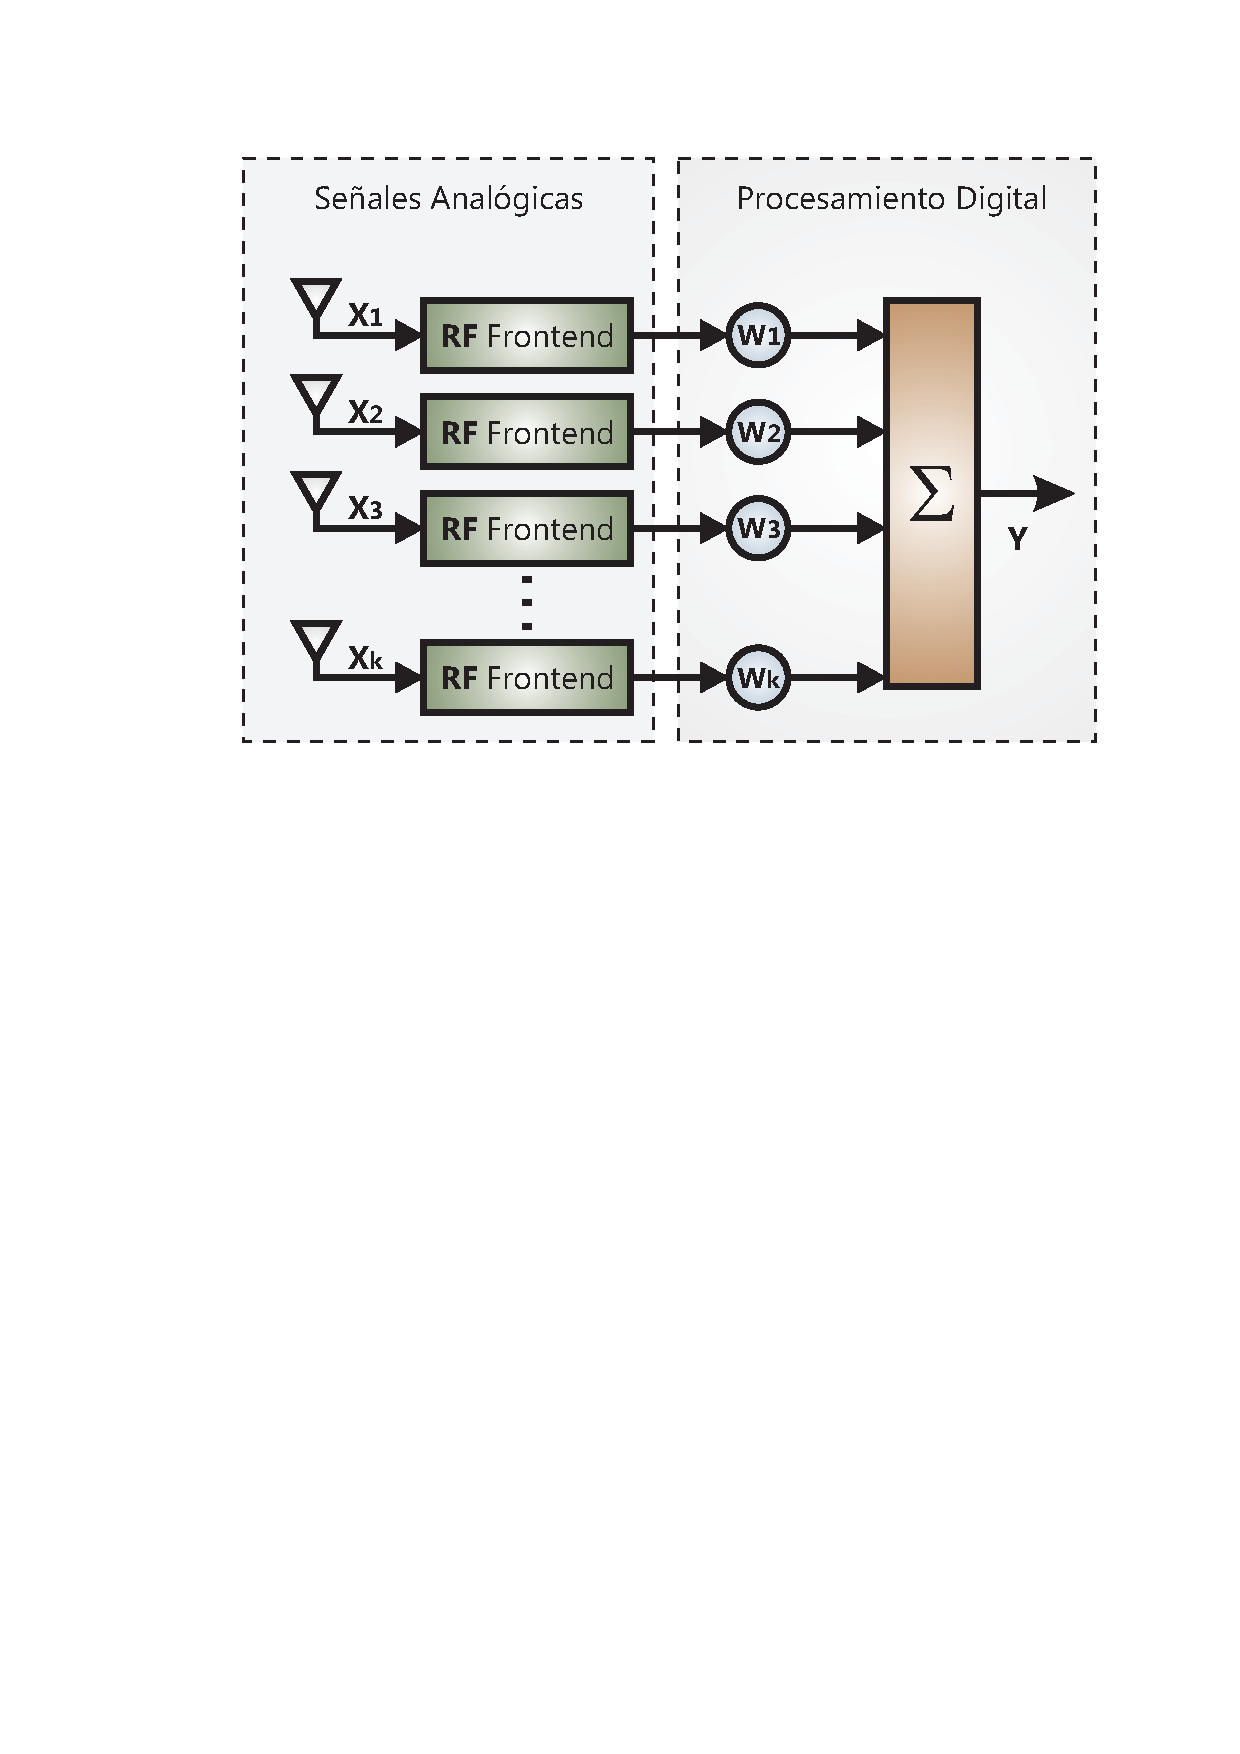
\includegraphics[width=10cm]{./figures/C02-beamforming}
%         \caption{Esquema de un sistema de \textit{Beamforming}}
%         \label{fig:Beamforming}
% \end{figure}
% 
% Se puede observar en la \textbf{figura \ref{fig:Beamforming}} que las señales provenientes de cada una de las antenas son registradas por un frontend de RF en el cual se considera que está presente toda la circuitería analógica requerida para adaptar la señal y el conversor A/D utilizado para transformarla a un stream digital. Las señales digitales obtenidas ingresan luego al procesador digital en el cual se implementan los pesajes $w_1, w_2, ..., w_k$ para obtener una suma ponderada de las mismas.
% 
% Tanto la amplitud como la fase de cada antena pueden ser controladas. La combinación del control de fase y amplitud puede ser utilizada para ajustar los lóbulos laterales y dirigir nulos mejor que lo que se puede lograr con el control de fase por si solo. La amplitud relativa $a_k$ y desplazamiento de fase $\theta_k$ para cada antena es llamado un ``peso complejo'' y es representado por una constante compleja $w_k$ (para la antena en la $k^{\text{ésima}}$ posición)
% 
% Un \textit{beamformer} para un transmisor de radio aplica los coeficientes de ponderación a la señal a transmitir (desplaza la fase y aplica la amplitud) para cada elemento del arreglo de antenas.
% 
% Un \textit{beamformer} para la recepción en radio aplica los pesos complejos a la señal de cada antena, y luego suma todas las señales para formar aquella que tiene el patrón direccional deseado.
% 
% Las primeras ideas que formaron las bases del \textit{beamforming} digital fueron desarrolladas por investigadores en las áreas de sistemas de radar y sonar. El \textit{beamforming} digital es una unión entre las tecnologías de antena y las tecnologías digitales. Una antena puede ser considerada un dispositivo que convierte señales espacio-temporales en señales estrictamente temporales, haciéndolas disponibles a una gran variedad de técnicas de procesamiento de señales. De esta forma, toda la información deseada que está siendo transportada por estas señales puede ser extraída.
% 
% Una ventaja mayor del \textit{beamforming} digital radica en el hecho de que una vez que la información de RF es capturada en la forma de un flujo digital, dicho contenido está disponible para la aplicación de una gran cantidad de técnicas de procesamiento digital de señales. 
% 
% El haz deseado es formado en el dominio digital (dentro del sistema de procesamiento). Para diseñar el sistema de procesamiento pueden utilizarse distintas tencologías, tales como FPGA, DSPs de propósito general o chips específicamente diseñados para \textit{beamforming}. El procesamiento digital requiere que la señal de cada antena sea digitalizada utilizando un conversor A/D. Debido a que las señales de radio por encima de las frecuencías de onda corta ($>30 MHz$) son muy altas para ser digitalizadas directamente a un costo razonable, los receptores de \textit{beamforming} digital utilizan ``traductores de RF'' para desplazar la frecuencia de la señal hacia niveles inferiores antes de los conversores A/D. La clave de esta tecnología es lograr una traducción precisa de la señal analógica al régimen digital. Esto se logra utilizando receptores heterodinos completos, los cuales deben estar cercanamente apareados en amplitud y fase. Los receptores deben realizar el pasaje a frecuencias inferiores, filtrado y amplificación a un nivel de potencia adaptado a los requerimientos de entrada de los conversores A/D.
% 
% 
% \subsection{\textit{Beamforming} adaptativo}
% 
% Un \textit{beamformer} adaptativo es un dispositivo que tiene la capacidad de separar señales en el dominio del espacio. Este hecho provee un medio para separar la señal deseada de señales de interferencia. Un \textit{beamformer} adaptativo logra optimizar automaticamente el patrón del arreglo al ajustar el control de los pesos de ponderación hasta que se satisface una determinada función de objetivo prestablecida. Los medios por los cuales esta optimización es lograda están especificados por un algoritmo diseñado para tal propósito. Estos dispositivos utilizan mucha más información disponible en la antena con respecto a un \textit{beamformer} convencional.
% 
% \begin{figure}[htb!]
%         \centering
%         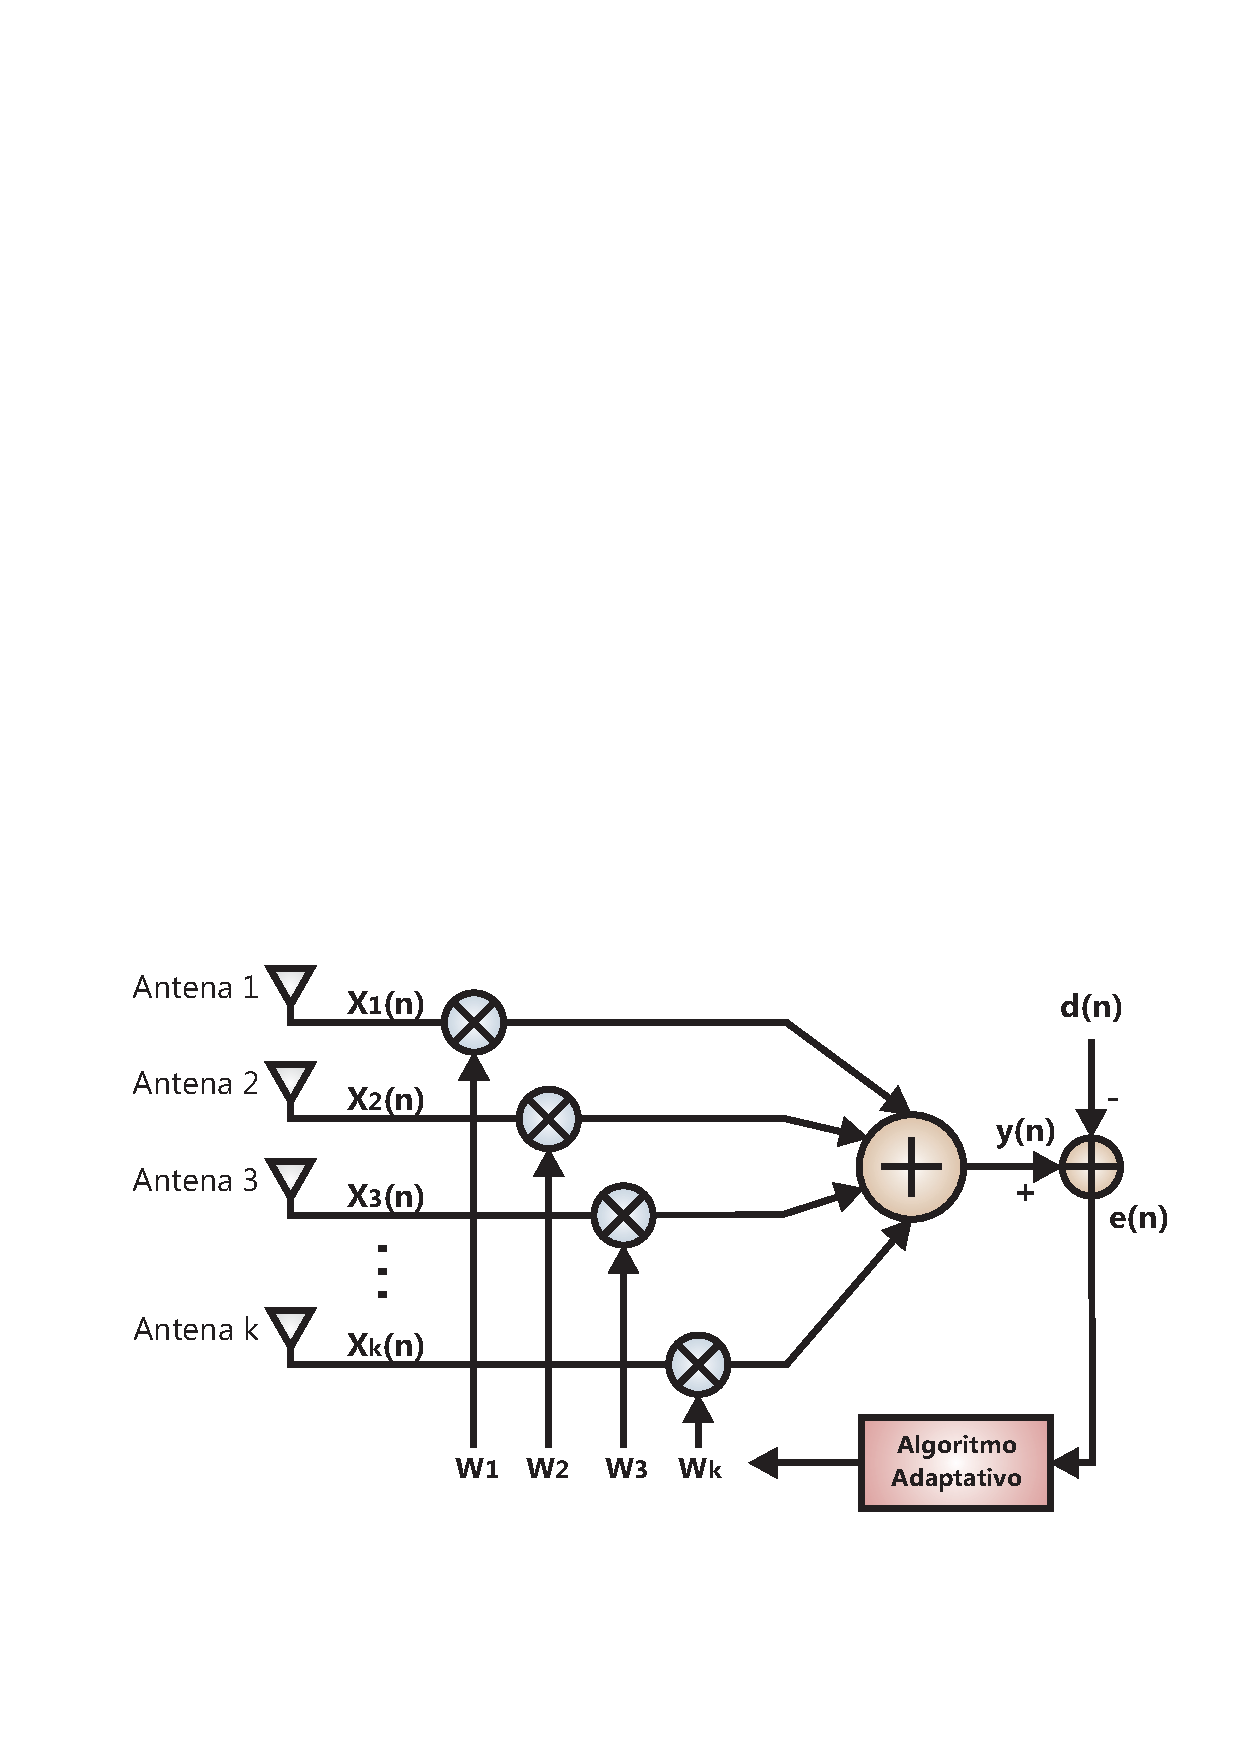
\includegraphics[width=10cm]{./figures/C02-adaptive_beamforming}
%         \caption{Esquema de un sistema de \textit{Beamforming} Adaptativo}
%         \label{fig:Adaptive_Beamforming}
% \end{figure}
% 
% \subsubsection{Conceptos básicos}
% 
% El procedimiento utilizado para direccionar y modificar el patrón del haz del arreglo con el objetivo de mejorar la recepción de la señal deseada, mientras simultáneamente se suprimen las señales de interferencia a través de la seleción de pesos complejos, se puede exponer como se explica a continuación.
% 
% Se tiene un arreglo como el expuesto en la figura \ref{fig:example}, que consiste de dos antenas omnidireccionales con espaciado $\lambda_0/2$. La señal deseada, $S(t)$ llega desde la dirección de máxima ganancia ($\Theta_S = 0$), y la señal de interferencia, $I(t)$ llega desde el ángulo ($\Theta_1 = \pi / 6$).
% 
% \begin{figure}[htb!]
%         \centering
%         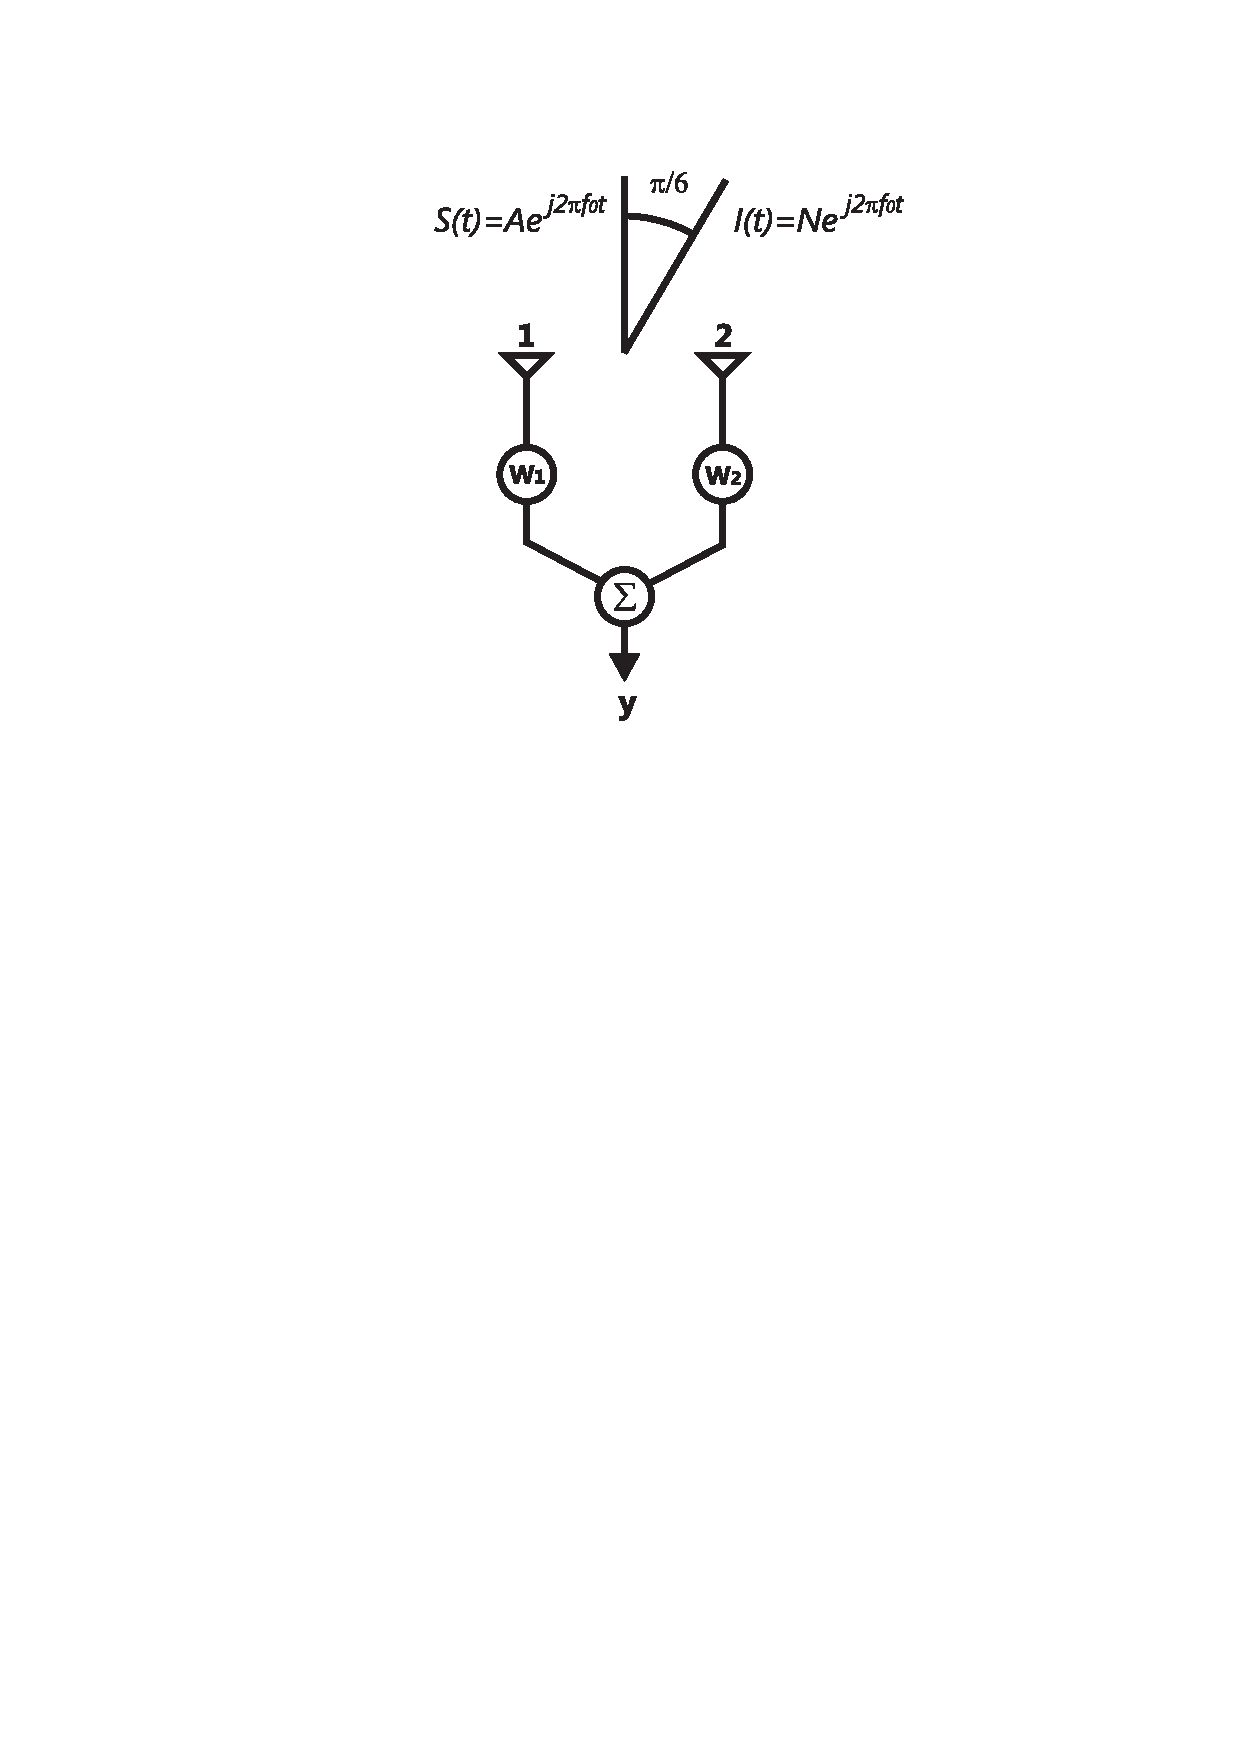
\includegraphics[width=7cm]{./figures/C02-example}
%         \caption{Arreglo de dos elementos para la supresión de interferencia}
%         \label{fig:example}
% \end{figure}
% 
% Ambas señales tienen la misma frecuencia $f_o$. La señal de cada antena es multiplicada por una variable de ponderación compleja, y las señales ponderadas son luego sumadas para formar la salida del arreglo. La contribución de señal deseada en la salida del arreglo es:
% 
% \begin{equation}
% y_d(t) = A e^{j 2 \pi f_o t}(w_1 + w_2)
% \end{equation}
% 
% Para que $y_d(t)$ sea igual a S(t), es necesario que
% 
% \begin{equation}
% \begin{array}{l}
% \Re[w_1] + \Re[w_2] = 1\\
% \Im[w_1] + \Im[w_2] = 0 \label{desired_condition1}
% \end{array}
% \end{equation}
% 
% Donde $\Re[]$ e $\Im[]$ corresponden a las componentes real e imaginaria respectivamente. La señal de interferencia incidente llega al elemento 2 con una dirección de fase con respecto al elemento 1 de valor $2 \pi \frac{1}{\lambda_0} d sin (\pi / 6) = \pi / 2$. Consecuentemente, la contribución de señal de interferencia en la salida del arreglo es:
% 
% \begin{equation}
% y_i(t) = N e^{j 2 \pi f_o t}w_1 + N e^{(j 2 \pi f_o t + \pi / 2)} w_2 
% \end{equation}
% 
% Para que la respuesta de interferencia del arreglo sea cero es necesario que
% 
% \begin{equation}
% \begin{array}{l}
% \Re[w_1] + \Re[jw_2] = 0\\
% \Im[w_1] + \Im[jw_2] = 0 \label{desired_condition2}
% \end{array}
% \end{equation}
% 
% La solución simultánea para las ecuaciones \eqref{desired_condition1} y \eqref{desired_condition2} lleva a:
% 
% \[
% w_1 = \frac{1}{2} - j \frac{1}{2} \hspace{3cm} w_2 = \frac{1}{2} + j \frac{1}{2}
% \]
% 
% Con estos pesos, el arreglo aceptará la señal deseada mientras que simultáneamente rechazará la interferencia.
% 
% El ejemplo expuesto toma ventaja en el hecho de que sólo hay un único origen de interferencia direccional y que utiliza la información a priori sobre la frecuencia y dirección de ambas señales. Un procesador práctico no debería requerir ese nivel de detalles en la información a priori sobre la ubicación, número y naturaleza de las fuentes de señal.
% 
% De todas formas, el ejemplo muestra que un sistema compuesto por un arreglo, que es configurado con pesos complejos, provee posibilidades innumerables para realizar los objetivos del sistema. Sólo se necesita desarrollar un procesador adaptativo práctico para llevar a cabo el ajuste en los pesos complejos.
% 
% \subsection{Criterios para obtener los pesos óptimos}
% 
% A continuación se mencionan algunos criterios existentes para la elección de los pesos óptimos para el filtro adaptativo. Se verá que cada uno de ellos se puede expresar como una solución a la \textbf{ecuación de Wiener Hopf}.
% 
% \subsubsection{Mínimo error cuadrático medio}
% 
% Considerar inicialmente un arreglo de antenas uniformemente espaciado, el cual opera en un ambiente de señal donde se tiene una señal de comunicación desada $s(t)$, así como tambien $N_u$ señales de interferencia $\{u_i(t)\}^{N_u}_{i=1}$. Luego considerar que las señales deseadas llegan al arreglo con un ángulo espacial $\theta_0$ y que la señal de interferencia $i$ llega con un ángulo $\theta_i$. La salida del arreglo es representada por:
% 
% \begin{equation}
% \mathbf{x}(t) = s(t) \mathbf{v} + \mathbf{u} = \mathbf{s} + \mathbf{u}
% \end{equation}
% 
% $\mathbf{v}$ consiste en el vector de propagación del arreglo para la señal deseada:
% 
% \begin{equation}
% \mathbf{v}^T = [1,e^{j k d sin \theta_0} ... e^{j k (K-1) d sin \theta_0}]
% \end{equation}
% 
% $\mathbf{u}$ representa la suma de todos los vectores de señales de interferencia:
% 
% \begin{equation}
% \mathbf{u}^T = \sum_{i=1}^{N_u} u_i(t) \boldsymbol\eta_i
% \end{equation}
% 
% y $\boldsymbol\eta_i$ es el vector de propagación del arreglo para la $i^{\text{ésima}}$ señal de interferencia.
% 
% \begin{equation}
% \boldsymbol\eta_i^T = [1, e^{j k d sin \theta_i} ... e^{j k (K-1) d sin \theta_i}]
% \end{equation}
% 
% Si la señal deseada $s(t)$ es conocida, uno puede elegir minimizar el error entre la salida del \textit{beamformer} $\mathbf{w}^H \mathbf{x}(t)$ y la señal deseada. Por supuesto, el conocimiento de la señal deseada eliminiaría la necesidad del \textit{beamformer}. De todas formas, para muchas aplicaciones, las características de la señal deseada pueden ser conocidas con suficiente detalle para generar una señal $d^*(t)$ que la representa cercanamente, o que por lo menos se correlaciona con la señala deseada en un cierto nivel. Esta señal es llamada la \textbf{señal de referencia}. Se expresa a la señal de referencia como un complejo conjugado sólo por conveniencia matemática. Los pesos son elegidos para minimizar el error cuadrático medio (MSE) entre la salida del \textit{beamformer} y la señal de referencia:
% 
% \begin{equation}
% \epsilon^2(t) = [d^*(t) - \mathbf{w}^H \mathbf{x}(t)]^2
% \label{mse}
% \end{equation}
% 
% Al tomar la esperanza en ambos lados de la ecuación \eqref{mse} y llevar a cabo algunas manipulaciones algebráicas, se tiene:
% 
% \begin{equation}
% E\{\epsilon^2(t)\} = E\{d^*(t)\} - 2 \mathbf{w}^H \mathbf{r} + \mathbf{w}^H \mathbf{R} \mathbf{w}
% \label{mse_E}
% \end{equation}
% 
% donde $\mathbf{r} = E\{d^*(t)x(t)\}$ y $\mathbf{R} = E\{\mathbf{x}(t)\mathbf{x}^H(t)\}$. $\mathbf{R}$ es usualmente referida como la matriz de covarianza. El mínimo error cuadrático medio se obtiene al igualar a cero el gradiente del vector de la ecuación \eqref{mse_E} con respecto a $\mathbf{w}$.
% 
% \begin{equation}
% \nabla \mathbf{w} (E\{ \epsilon^2(t)\}) = -2 \mathbf{r} + 2 \mathbf{R} \mathbf{w} = 0
% \label{nabla_to_zero}
% \end{equation}
% 
% La solución a esta ecuación es
% 
% \begin{equation}
% \mathbf{w}_{opt} = \mathbf{R}^{-1} \mathbf{r}
% \label{wiener}
% \end{equation}
% 
% la cual es referida como la ecuación de Wiener-Hopf o la solución óptima Wiener. Si $s(t) = d^*(t)$ luego $\mathbf{r} = E\{d^2(t)\} \mathbf{v}$. Se puede expresar $\mathbf{R} = E\{d^2(t)\} \mathbf{v v^H} + \mathbf{R}_u$, donde $\mathbf{R}_u = E\{\mathbf{u u^H}\}$ y aplicar la \textit{Identidad de Woodbury} a $\mathbf{R^{-1}}$ y se tiene:
% 
% \begin{equation}
% \mathbf{R^{-1}} = \Bigg[ \frac{1}{1 + E\{d^2(t)\} \mathbf{v^H R_u^{-1} v}} \Bigg] \mathbf{R_u^{-1}}
% \end{equation}
% 
% Luego, la solución de Wiener se puede generalizar como:
% 
% \begin{equation}
% \mathbf{w}_{\text{opt}} = \beta \mathbf{R_u^{-1}v}
% \end{equation}
% 
% Donde $\beta$ es el coeficiente escalar. En el caso del mínimo MSE:
% 
% \begin{equation}
% \beta = \frac{E\{d^2(t)\}}{1 + E\{d^2(t)\} \mathbf{v^H R_u^{-1} v}}
% \end{equation}
% 
% \subsubsection{Máxima relación señal interferencia}
% 
% Los pesos pueden ser elegidos para maximizar la relación señal interferencia (SIR). Si se asume que $\mathbf{R_s} = E\{\mathbf{s s^H}\}$ y $\mathbf{R_u} = E\{\mathbf{u u^H}\}$ son conocidas, se puede elegir maximizar la relación de la potencia de señal de salida $\sigma_s^2$ y el total de potencial de señal de interferencia $\sigma_u^2$. La potencia de señal de salida puede expresarse como:
% 
% \begin{equation}
% \sigma_s^2 = E\{|\mathbf{w^H s}|^2\} = \mathbf{w^H R_s w}
% \end{equation}
% 
% y la potencia de salida de ruido como:
% 
% \begin{equation}
% \sigma_u^2 = E\{|\mathbf{w^H u}|^2\} = \mathbf{w^H R_u w}
% \end{equation}
% 
% Luego, la SIR está dada por:
% 
% \begin{equation}
% \text{SIR} = \frac{\sigma_s^2}{\sigma_u^2} = \frac{\mathbf{w^H R_s w}}{\mathbf{w^H R_u w}}
% \label{SIR}
% \end{equation}
% 
% Tomando la derivada de (\ref{SIR}) con respecto a $\mathbf{w}$ e igualándola a cero se obtiene:
% 
% \begin{equation}
% \mathbf{R_s w} = \frac{\mathbf{w^H R_s w}}{\mathbf{w^H R_u w}} \mathbf{R_u w}
% \end{equation}
% 
% lo cual consiste en un problema de autovalores. El valor de $\frac{\mathbf{w^H R_s w}}{\mathbf{w^H R_u w}}$ está delimitado por los autovalores mínimo y máximo de la matriz simétrica $\mathbf{R_u^{-1} R_s}$. El máximo autovalor $\lambda_{\text{max}}$ que satisface
% 
% \begin{equation}
% \mathbf{R_u^{-1} R_s w} = \lambda_{\text{max}} \mathbf{w}
% \end{equation}
% 
% es el óptimo valor de SIR. Correspondiente a este valor, existe un único autovector, $w_{\text{opt}}$ que representa a los pesos óptimos. Luego:
% 
% \begin{equation}
% \mathbf{R_s w_{\text{opt}}} = \text{SIR} \hspace{1mm} \mathbf{R_u w_{\text{opt}}}
% \end{equation}
% 
% Notando que $\mathbf{R_s} = E\{d^2(t)\} \mathbf{v v^H}$, se obtiene:
% 
% \begin{equation}
% \mathbf{w}_{\text{opt}} = \beta \mathbf{R_u^{-1}v}
% \end{equation}
% 
% donde
% 
% \begin{equation}
% \beta = \frac{E\{d^2(t)\}}{\text{SIR}} \mathbf{v^H w_\text{opt}}
% \end{equation}
% 
% Lo cual representa que el criterio del máximo SIR puede ser también expresado en términos de la solución de Wiener.
% 
% \subsubsection{Varianza mínima}
% 
% Si la señal deseada y su dirección son desconocidas, una forma de asegurar una buena recepción de señal es minimizar la varianza del ruido de salida. Recordando que la salida del \textit{beamformer} es:
% 
% \begin{align}
% y(t) &=  \mathbf{w^H x} \\
%      &=  \mathbf{w^H s + w^H u} \nonumber
% \end{align}
% 
% Para asegurar que la señal deseada es enviada con una ganancia y fase específica, se puede utilizar una restricción de forma que la respuesta del \textit{beamformer} para la señal deseada sea:
% 
% \begin{equation}
% \mathbf{w^H v} = g
% \label{constraint}
% \end{equation}
% 
% La minimización de las contribuciones a la salida a causa de la interferencia es lograda a través de la elección de los pesos para minimizar la varianza de la potencia de salida
% 
% \begin{align}
% \text{Var}\{y\} &=  \mathbf{w^H R w} \\
%                 &=  \mathbf{w^H R_s w + w^H R_u w} \nonumber 
% \end{align}
% 
% sujeta a la restricción definida en (\ref{constraint}). Esto es equivalente a minimizar la cantidad $\mathbf{w^H R_u w}$. Utilizando el método de Lagrange, se tiene
% 
% \begin{equation}
% \mathbf{\nabla w}\Bigg(\frac{1}{2} \mathbf{w^H R_u w} + \beta [1 - \mathbf{w^H v}]\Bigg) = \mathbf{R_u w} - \beta \mathbf{v}
% \end{equation}
% 
% de forma tal que
% 
% \begin{equation}
% \mathbf{w}_\text{opt} = \beta \mathbf{R_u^{-1} v}
% \label{variance_solution}
% \end{equation}
% 
% donde
% 
% \begin{equation}
%  \beta = \frac{g}{\mathbf{v^H R_u^{-1} v}}
% \end{equation}
% 
% La solución \ref{variance_solution} es también una solución de Wiener. Si $g = 1$, la respuesta del \textit{beamformer} es normalmente conocida como la respuesta de mínima varianza sin distorción (MVDR).
% 
% \section{Algoritmos adaptativos}
% 
% En la sección anterior, se mostró que los criterios óptimos estan íntimamente relacionados entre si. Por lo cual, la elección del criterio no es crítica en términos de rendimiento.
% 
% Por otro lado, la elección de \textbf{algoritmos adaptativos} para derivar los pesos adaptativos es muy importante, dado que determina tanto la velocidad de convergencia como la complejidad de hardware requerida para implementar el algoritmo. A continuación se discutiran algunas de las técnicas adaptativas más comunes.
% 
% \subsection{Algoritmo LMS - \textit{Least Mean Squares}}
% 
% El algoritmo adaptativo más común para adaptatividad continua es el \textbf{algoritmo LMS}. Se basa en el método de descenso más pronunciado, que computa y actualiza recursivamente el vector de pesos. Es razonablemente intuitivo que correcciones sucesivas al vector de pesos en la dirección negativa del vector gradiente deberían eventualmente llevar al MSE, hasta un punto tal que el vector de pesos asume su valor óptimo. De acuerdo al método, el valor actualizado del vector de pesos en el momento $n + 1$ es computado utilizando la siguiente relación recursiva simple
% 
% \begin{equation}
% \mathbf{w}(n + 1) \approx \mathbf{w}(n) + \frac{1}{2} \mu [-\mathbf{\nabla}(E\{\epsilon^2(n)\})]
% \end{equation}
% 
% Reemplazando con (\ref{nabla_to_zero}) se obtiene
% 
% \begin{equation}
% \mathbf{w}(n + 1) = \mathbf{w}(n) + \mu [\mathbf{r} - \mathbf{R w}(n)]
% \end{equation}
% 
% En la realidad, una medición exacta del vector gradiente no es posible, dado que esto requeriría un conocimiento previo tanto de $\mathbf{R}$ como de $\mathbf{r}$. La estrategia más obvia consiste en usar estimaciones instantáneas, las cuales son definidas respectivamente como:
% 
% \begin{equation}
% \mathbf{\hat{R}}(n) = \mathbf{x}(n) \mathbf{x}^H(n)
% \end{equation}
% 
% y
% 
% \begin{equation}
% \mathbf{\hat{r}}(n) = \hat{d}(n) \mathbf{x}(n)
% \end{equation}
% 
% Los pesos pueden ser actualizados como
% 
% \begin{align}
% \mathbf{\hat{w}}(n + 1) &= \mathbf{\hat{w}}(n) + \mu \mathbf{x}(n)[\hat{d}(n) - \mathbf{x}^H(n)\mathbf{\hat{w}}(n)] \\
%                         &= \mathbf{\hat{w}}(n) + \mu \mathbf{x}(n) \hat{e}(n) \nonumber 
% \end{align}
% 
% La constante de ganancia $\mu$ controla las características de convergencia del vector de secuencia aleatorio $\mathbf{w}(n)$. Se debe notar que este es un enfoque continuamente adaptativo, en el cual los pesos son actualizados a medida que los datos son muestreados de forma tal que el vector resultante converja a la solución óptima. La adaptatividad continua funciona bien cuando las estadísticas relacionadas con el ambiente de la señal son \textbf{estacionarias}. La figura \ref{fig:lms_algorithm} muestra la representación gráfica del flujo de la señal del \textbf{algoritmo LMS}. La virtud principal de este algoritmo es su simplicidad. El rendimiento es aceptable en diversas aplicaciones. De todas formas, sus características de convergencia dependen en la estructura de autovalores de $\mathbf{\hat{R}}$. Cuando éstos están ampliamente difundidos, la convergencia puede ser lenta y debería considerarse utilizar otros algoritmos adaptativos con tasas de convergencia más altas.
% 
% \begin{figure}[htb!]
%         \centering
%         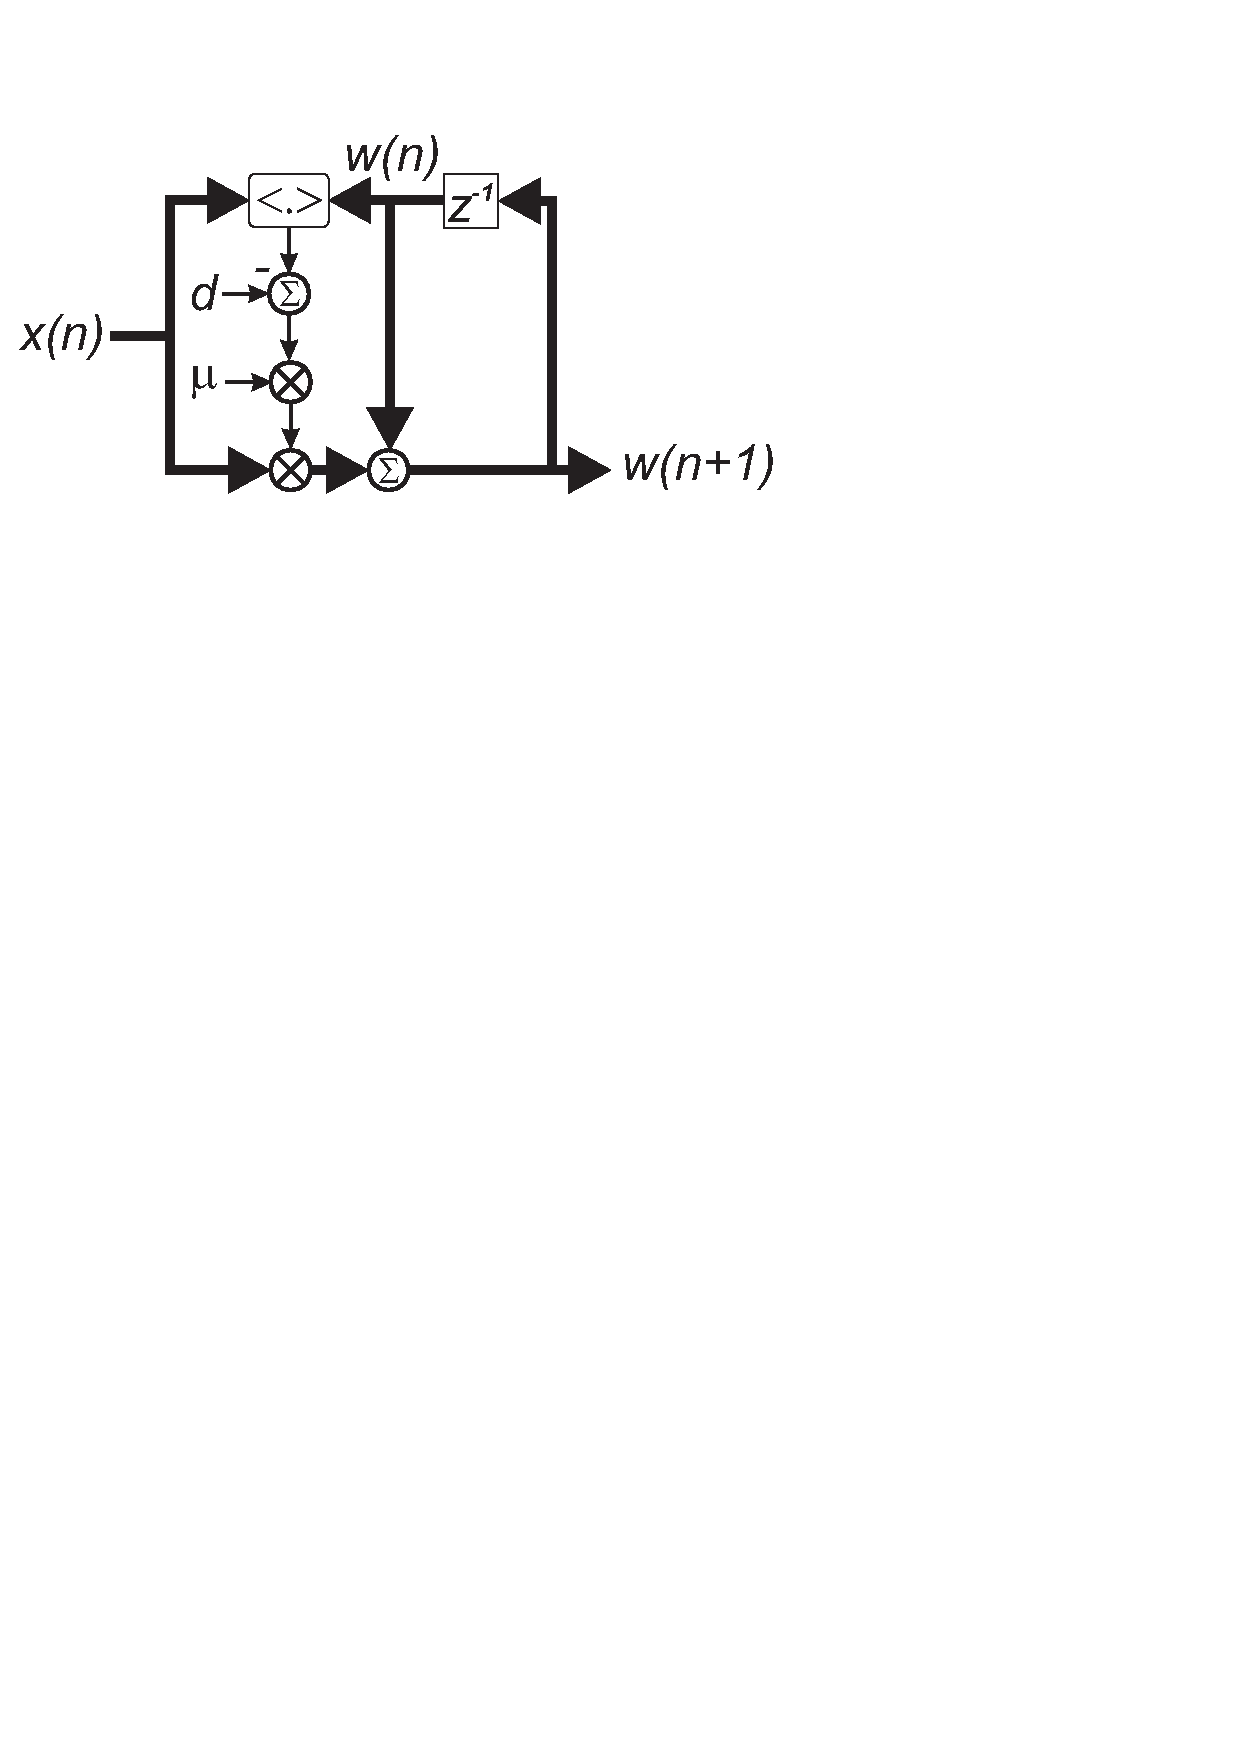
\includegraphics[width=6cm]{./figures/C02-lms_signal_flow}
%         \caption{Representación gráfica del flujo de señal para el algoritmo LMS}
%         \label{fig:lms_algorithm}
% \end{figure}
% 
% \subsection{Algoritmo RLS - \textit{Recursive Least Squares}}
% 
% En este algoritmo se realiza la estimación de $\mathbf{R}$ y $\mathbf{r}$ realizando una suma ponderada:
% 
% \begin{equation}
% \mathbf{\hat{R}}(n) = \sum_{i=1}^N \gamma^{n-1} \mathbf{x}(i) \mathbf{x}^H(i)
% \label{estimate_R}
% \end{equation}
% 
% y
% 
% \begin{equation}
% \mathbf{\hat{r}}(n) = \sum_{i=1}^N \gamma^{n-1} \hat{d}(i) \mathbf{x}(i)
% \label{estimate_r}
% \end{equation}
% 
% El factor de ponderación, $0 < \gamma \leq 1$ tiene la función de asegurar que los datos en el pasado son ``olvidados'' con el objetivo de permitir que el procesador siga las variaciones estadísticas de los datos observables. Factorizando los términos correspondientes a $i = n$ tanto en (\ref{estimate_R}) y (\ref{estimate_r}), se tiene la siguiente recursión para actualizar tanto $\mathbf{\hat{R}}(n)$ y $\mathbf{\hat{r}}(n)$:
% 
% \begin{equation}
% \mathbf{\hat{R}}(n) = \gamma \mathbf{R}(n-1) + \mathbf{x}(i) \mathbf{x}^H(n)
% \end{equation}
% 
% y
% 
% \begin{equation}
% \mathbf{\hat{r}}(n) = \gamma \mathbf{\hat{r}}(n-1) + \hat{d}(n) \mathbf{x}(n)
% \end{equation}
% 
% Utilizando la identidad de Woodbury, se puede obtener la siguiente ecuación recursiva para llegar a la inversa de la matriz de covarianza:
% 
% \begin{equation}
% \mathbf{R}^{-1}(n) = \gamma^{-1} [\mathbf{R}^{-1}(n-1) - \mathbf{q}(n) \mathbf{x}(n) \mathbf{R}^{-1}(n-1) ] 
% \end{equation}
% 
% donde el vector de ganancia $\mathbf{q}(n)$ está dado por:
% 
% \begin{equation}
% \mathbf{q}(n) = \frac{\gamma^{-1} \mathbf{R}^{-1}(n-1) \mathbf{x}(n)}{1 + \gamma^{-1} \mathbf{x}^H(n) \mathbf{R}^{-1}(n-1) \mathbf{x}(n)}
% \end{equation}
% 
% Para desarrollar la ecuación recursiva para actualizar el estimador de cuadrados mínimos $\mathbf{\hat{w}}(n)$ se usa (\ref{wiener}) para expresar $w(n)$ como sigue:
% 
% \begin{align}
% \mathbf{\hat{w}}(n) &= \mathbf{R}^{-1}(n) \mathbf{r}(n) \\
%                     &= \gamma^{-1} [ \mathbf{R}^{-1}(n-1) - \mathbf{q}(n)\mathbf{x}(n) \mathbf{R}^{-1}(n-1)] \nonumber \\
%                     &\qquad \times [\gamma \mathbf{r}(n-1) + \hat{d}(n) \mathbf{x}(n)]
%                     \nonumber
% \end{align}
% 
% Reorganizando la ecuación, se puede actualizar el peso como sigue:
% 
% \begin{equation}
% \mathbf{\hat{w}}(n) = \mathbf{\hat{w}}(n-1) + \mathbf{q}(n) [ \hat{d}(n) - \mathbf{\hat{w}}^H (n-1) \mathbf{x}(n) ]
% \end{equation}
% 
% Una característica importante del algoritmo RLS es que la inversión de la matriz de covarianza $\mathbf{x}(n)$ es reemplazada en cada paso por una división escalar simple. La figura \ref{fig:rls_algorithm} muestra la representación del flujo de señal del algoritmo RLS. La tasa de convergencia para el algoritmo RLS es típicamente un orden de magnitud más alta que la del algoritmo LMS.
% 
% \begin{figure}[htb!]
%         \centering
%         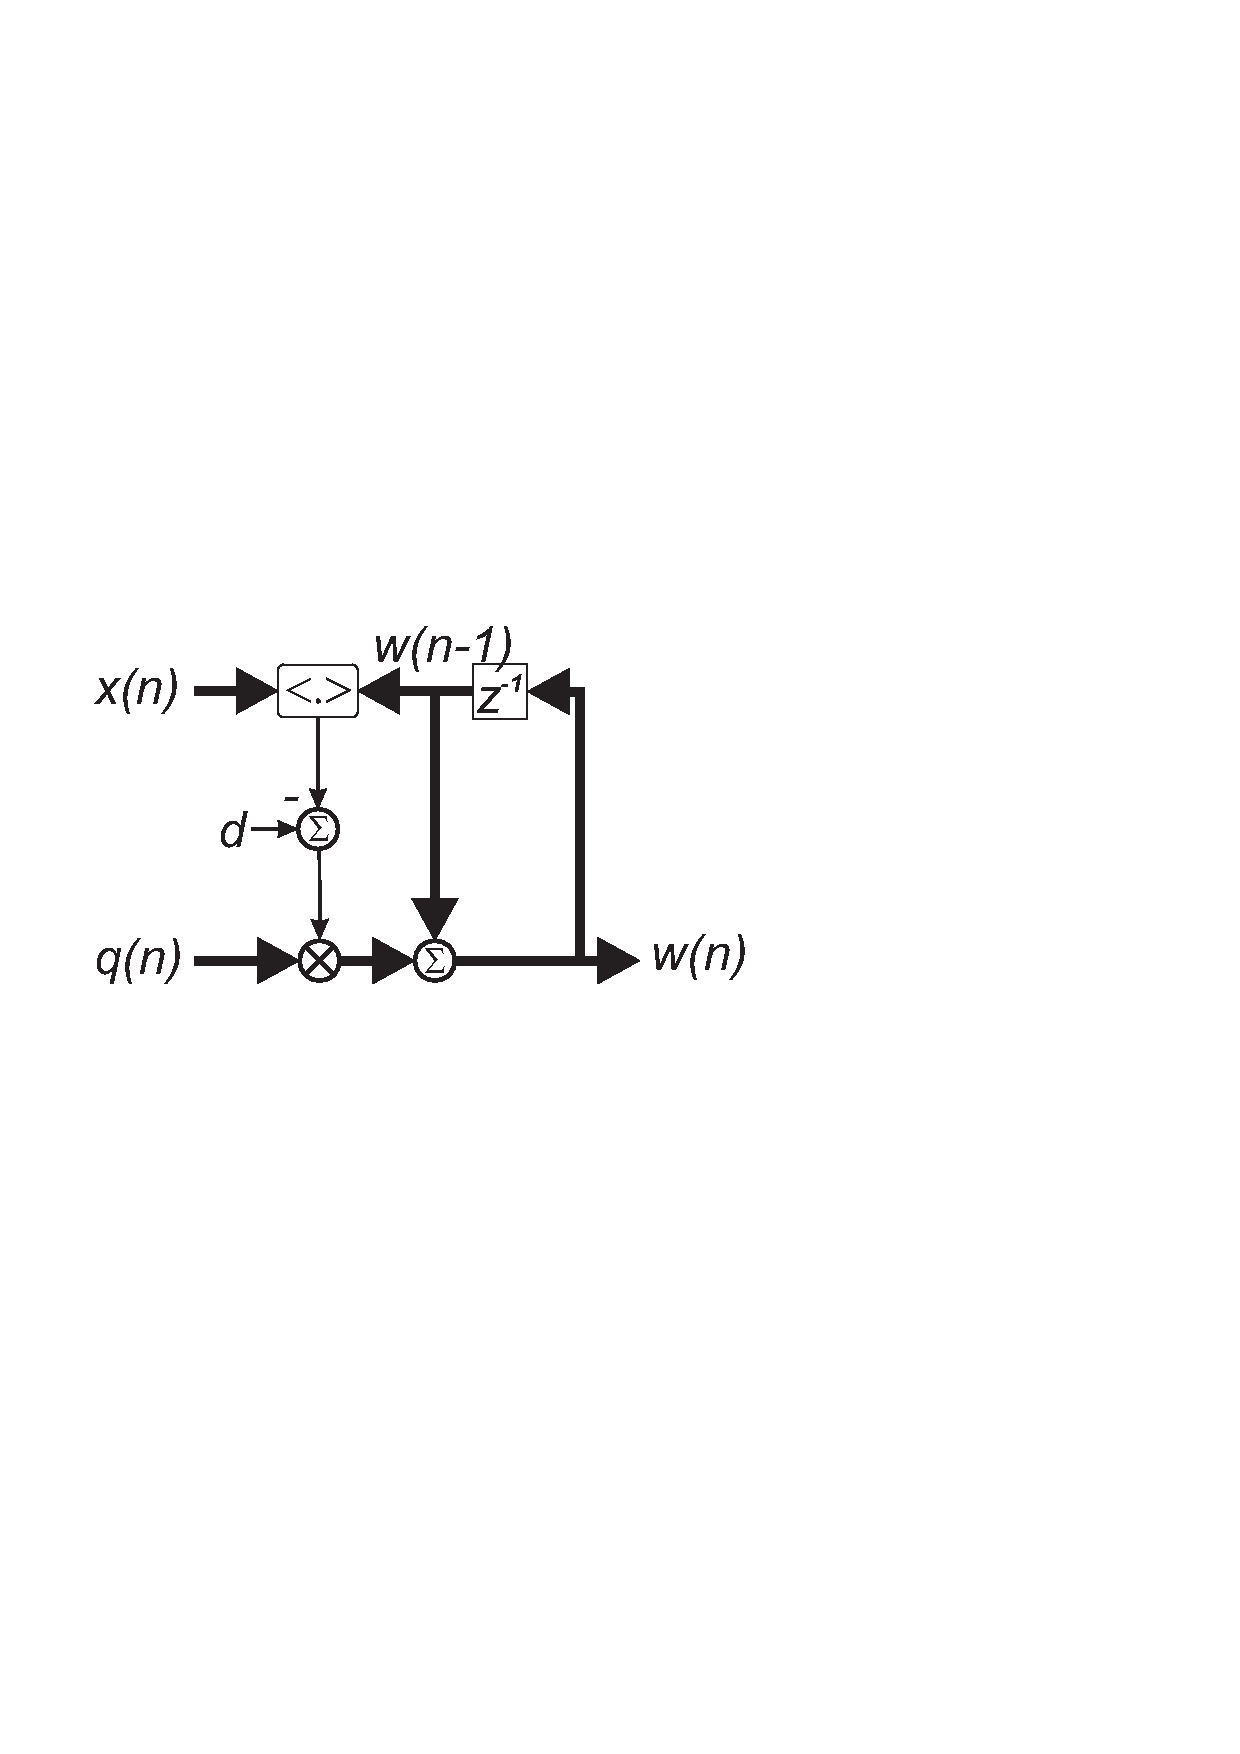
\includegraphics[width=6cm]{./figures/C02-rls_signal_flow}
%         \caption{Representación gráfica del flujo de señal para el algoritmo RLS}
%         \label{fig:rls_algorithm}
% \end{figure}
% 
% \subsection{Adquisición de la señal de referencia}
% 
% Se han planteado distintos criterios y algoritmos para realizar \textit{beamforming} adaptativo. Todos ellos requieren algún tipo de señal de referencia en su proceso de optimización adaptativa. Cuando se habla de señales de referencia, normalmente se refiere a información a priori y explícita o conocimientos sobre las señales de interés. Una referencia explícita puede ser dividida en dos categorías: referencia espacial y referencia temporal. La primera es refereida normalmente como la información de ángulo de arribo (AOA - \textit{Angle of Arrival}) de la señal deseada. Una señal de referencia temporal puede ser una señal piloto que está correlacionada con la señal deseada, una secuencia especial incluida en un paquete por la señal deseada, o un código pseudo-ruido (PN - \textit{pseudo-noise}) conocido en un sistema CDMA. La forma de referencia disponible depende del sistema particular donde se implementará el \textit{beamforming} adaptativo. Si una señal de referencia explícita está disponible en el sistema, se la debe ustilizar tanto como sea posible para lograr menor complejidad, mayor precisión y convergencia rápida.
% 
% Es valioso describir el proceso de adquisición de la señal de referencia en un sistema CDMA. El \textit{beamforming} adaptativo es muy adecuado para un sistema CDMA, debido a que los códigos de dispersión pueden ser usados como referencias para \textit{beamforming}. La implementación común de \textit{beamforming} adaptativo en un sistema de comunicaciones wireless CDMA es el uso del lazo de generación de referencia de Compton. Una configuración de implementación genérica para \textit{beamforming} adaptativo en CDMA se muestra en la figura \ref{fig:reference_signal_flow}. En esta configuración, la demodulación es realizada luego del \textit{beamforming}. Esto es, la salida del arreglo es primero mezclada con una señal de un oscilador local codificada CDMA, la cual es filtrada y limitada. La señal limitada es re-modulada a través de una mezcla con la señal del oscilador local codificado CDMA correspondiente.  La señal remodulada es usada como señal de referencia, la cual es comparada con la salida retrasada del arreglo para producir una señal de error. La señal de error dirige al procesador adaptativo para actualizar los pesos de \textit{beamforming}. El loop de retroalimentación es no lineal debido a la operación de limitación.
% 
% \begin{figure}[htb!]
%         \centering
%         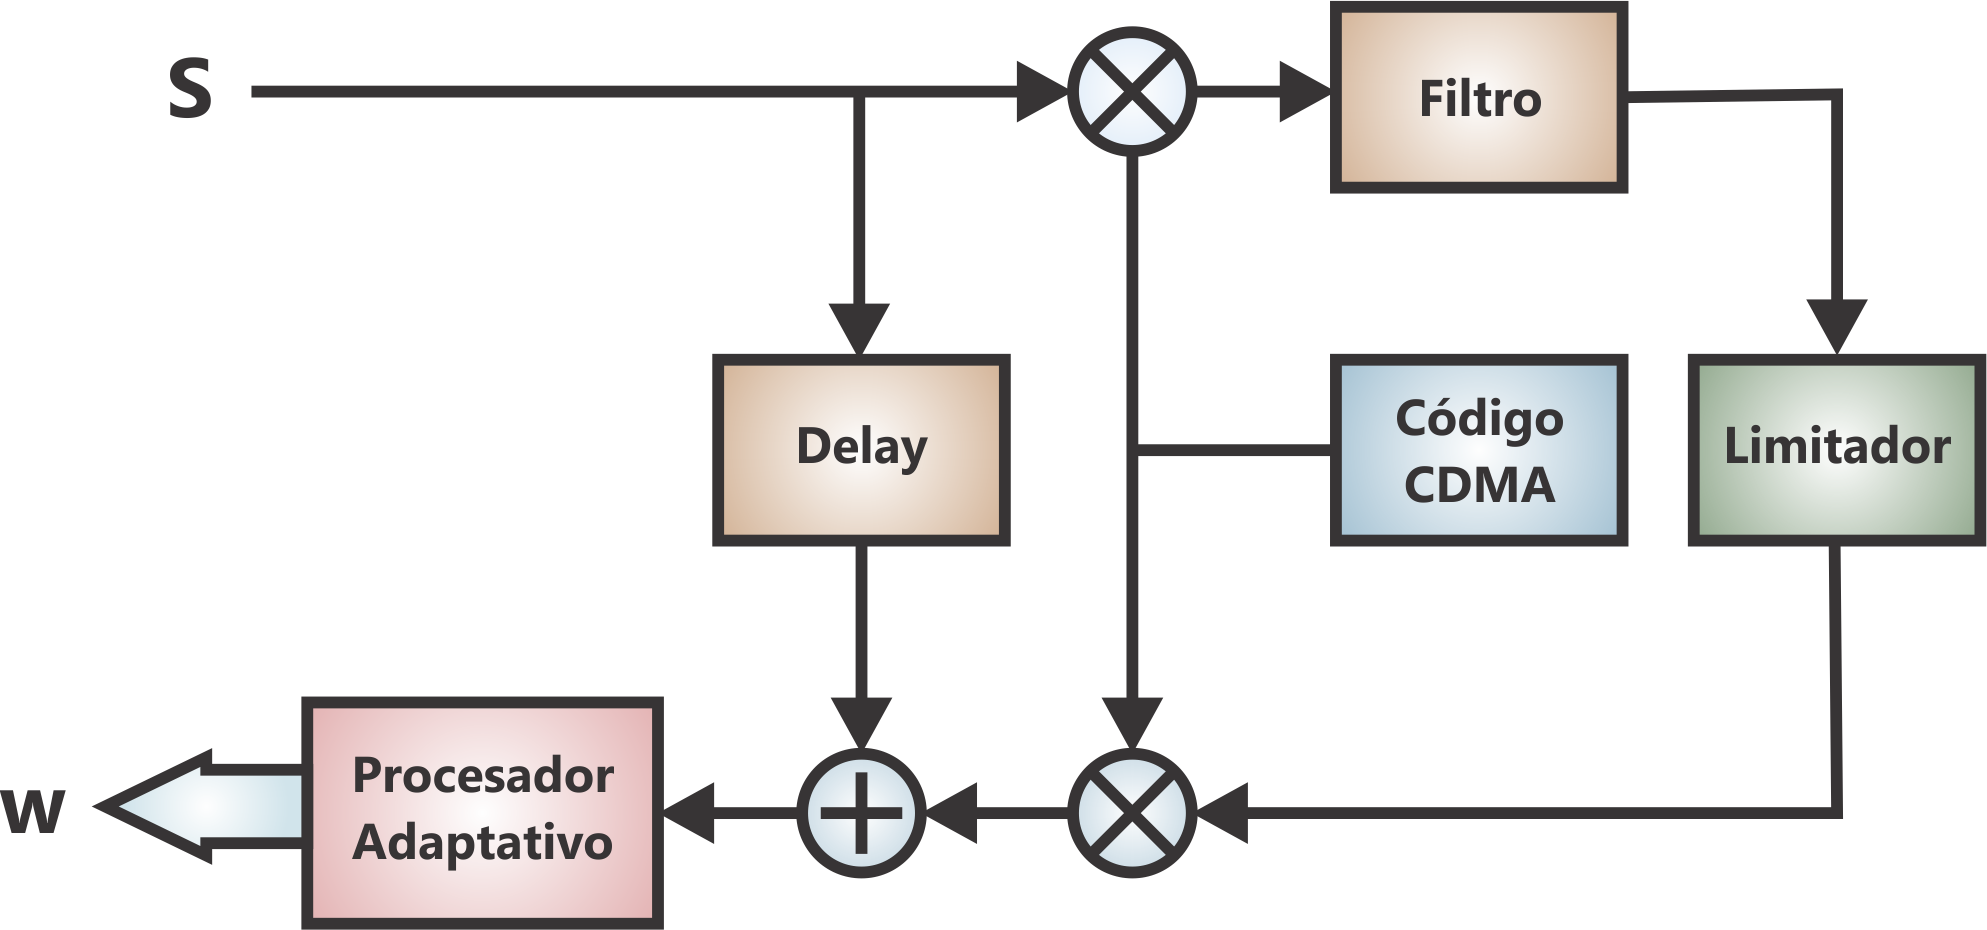
\includegraphics[width=9cm]{./figures/C02-reference_signal_flow}
%         \caption{Una configuración genérica para \textit{beamforming} adaptativo en un sistema de comunicación wireless CDMA}
%         \label{fig:reference_signal_flow}
% \end{figure}
% 
% \section{Otras técnicas de diseño MIMO}
% 
% Los sistemas MIMO pueden ser diseñados para proveer máxima diversidad para incrementar la confiabiliad de la transmisión, o para alcanzar una máxima ganancia de multiplexado para soportar altos niveles de tasas de transmisión.
% 
% La capacidad de un canal MIMO puede ser mucho más alta que la de un sistema SISO. Este rendimiento de un sistema MIMO es cuantificado a través de la ganancia de multiplexado espacial.
% 
% Si distintas copias de la señal son transmitidas o recibidas desde múltiples antenas, los sistemas pueden mejorar la confiabilidad de un enlace inalámbrico. Esta ganancia es llamada ganancia de diversidad.
% 
% Los sistemas MIMO pueden ser utilizados simultáneamente para proveer tanto ganancia por diversidad como por multiplexado. De todas formas, existe una relación de compromiso entre ellos.
% 
% \subsection{\textit{Space-Time block coding}}
% 
% En este tipo de diseño, se toman copias de la señal, las cuales son transmitidas desde múltiples antenas o son recibidas en más de una antena en sistemas multi-antena espacio-tiempo. La probabilidad de error promedio de símbolo de un sistema de comunicaciones MIMO para detección de máxima probabilidad tiene un límite superior en niveles altos de SNR \cite{Mohammadi2}:
% 
% \begin{equation}
% p_e \leq \overline{N_e}\Big(\frac{\gamma d_{min}}{4 M}\Big)^{-M}
% \end{equation}
% 
% donde $\overline{N_e}$ es el número de vecinos cercanos en una constelación escalar, $d_{min}$ es la distancia mínima de separación de la constelación escalar, y $M = min\{M_R,M_T\}$.
% 
% Como se puede ver en la figura \ref{fig:alamouti_chart}, incrementar el número de antenas aumenta la pendiente de las curvas del BER (bit error rate) y mejora la confiabilidad de la comunicación inalámbrica.
% 
% \begin{figure}[htb!]
%         \centering
%         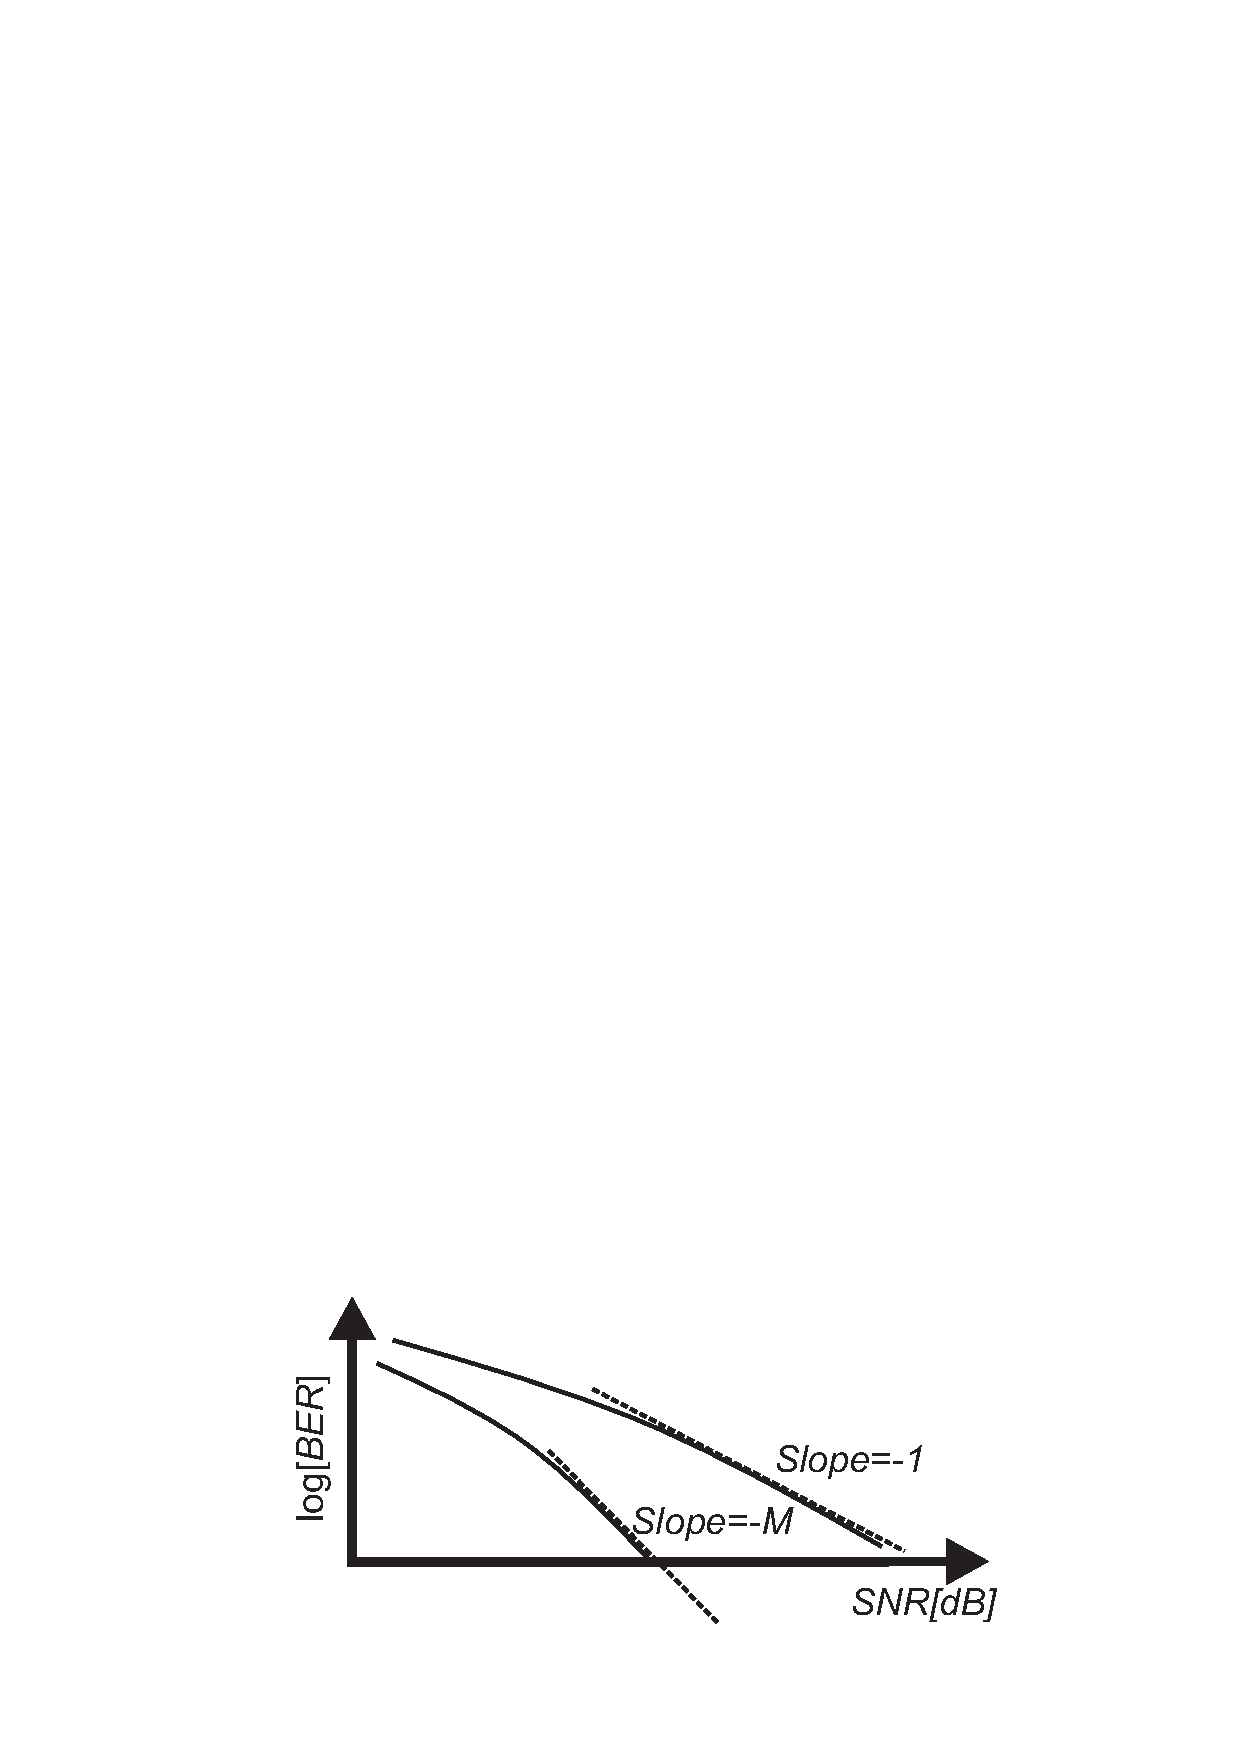
\includegraphics[width=6cm]{./figures/C02-alamouti_chart}
%         \caption{Ganancia de diversidad espacio-tiempo en sistemas MIMO}
%         \label{fig:alamouti_chart}
% \end{figure}
% 
% Uno de los ejemplos más claros de \textit{space-time block coding} es el conocido como código de Alamouti. El código de Alamouti es un space-time block code ortogonal (O-STBC). Es implementado utilizando dos antenas en el transmisor y un número arbitrario de antenas en el receptor. Las palabras del código para múltiples antenas son escritas de la siguiente forma:
% 
% \begin{equation}
% X = \frac{1}{\sqrt{2}}
% \left( \begin{array}{cc}
% \chi_1 & -\chi_2^* \\
% \chi_2 & \chi_1^* \end{array} \right)
% \end{equation}
% 
% El transmisor de Alamouti se muestra en la \ref{fig:alamouti}. El código de Alamouti tiene un rango de spatial multiplexing igual a uno, dado que se transmiten dos símbolos en el tiempo de duración de dos símbolos.
% 
% \begin{figure}[htb!]
%         \centering
%         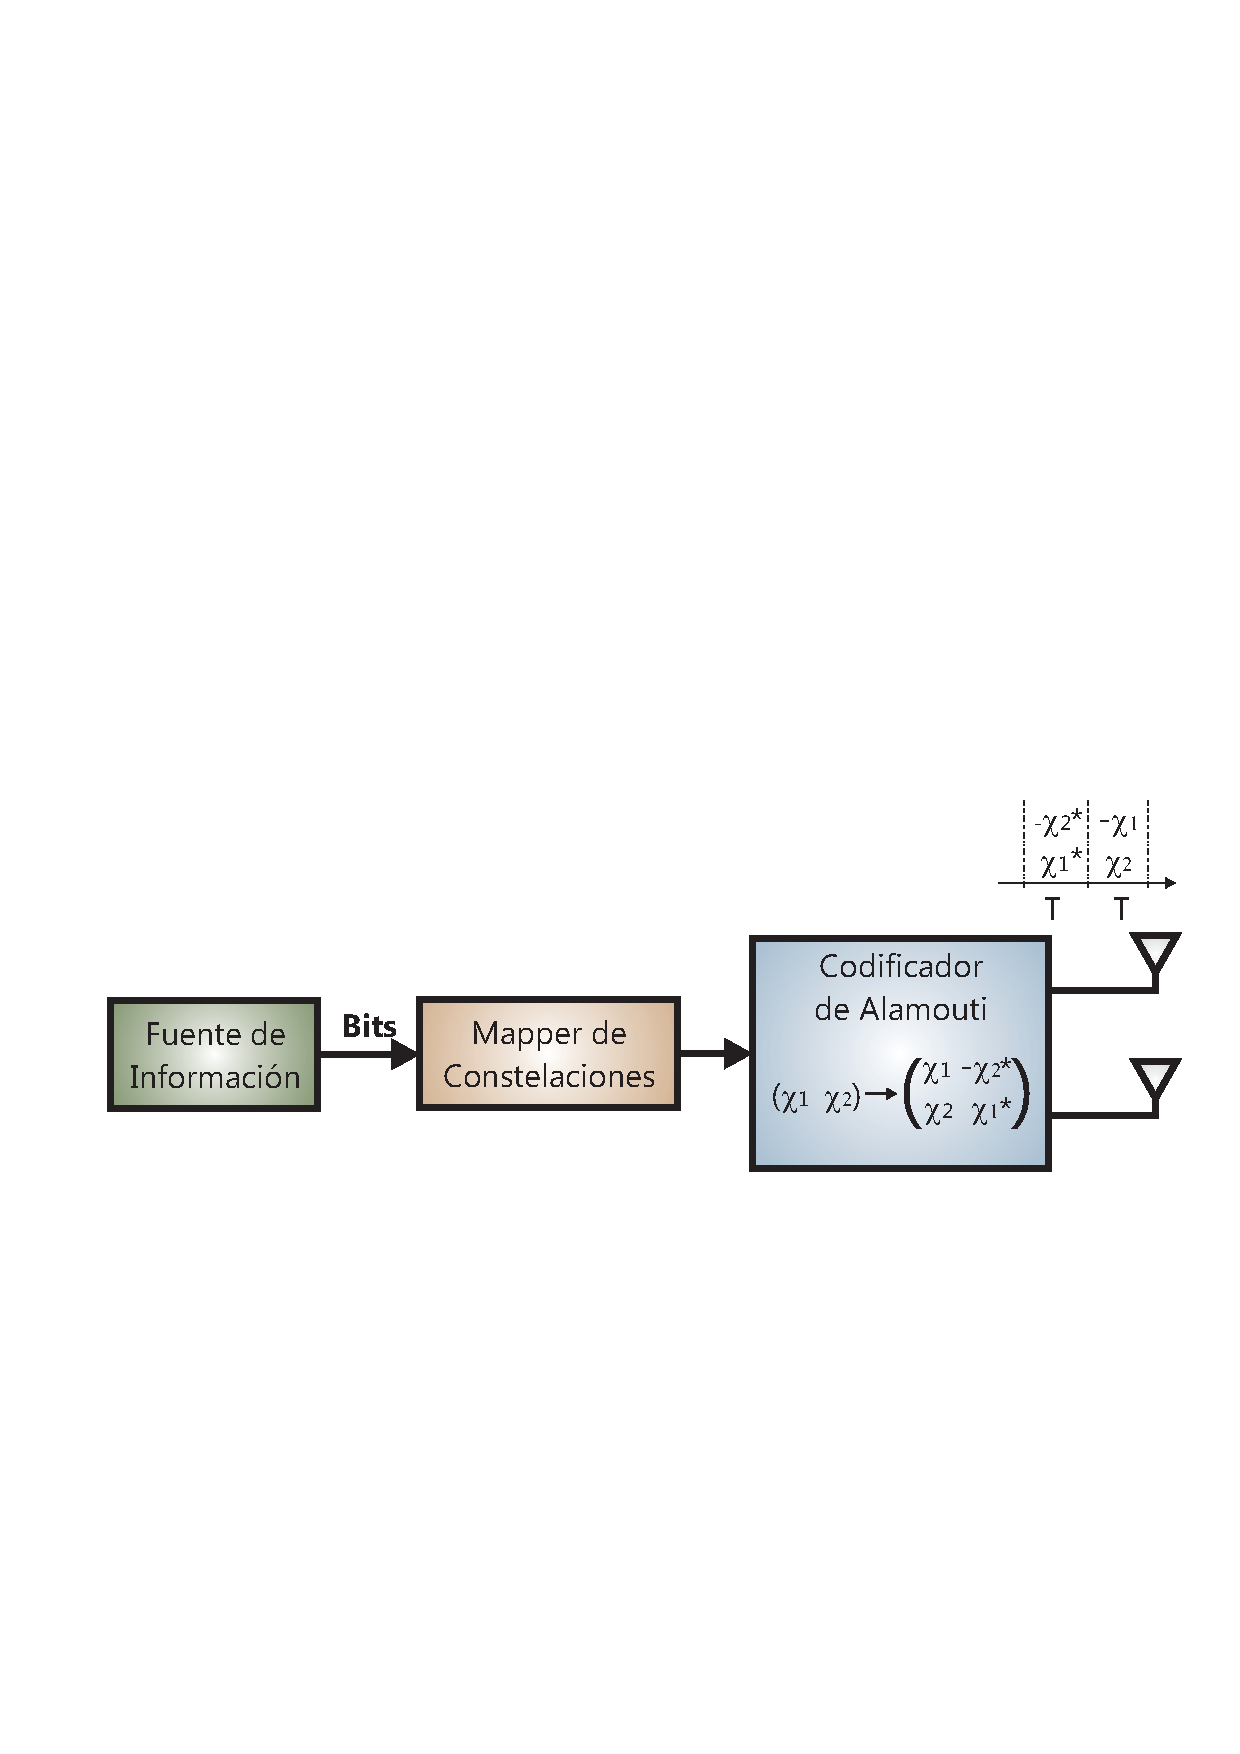
\includegraphics[width=10cm]{./figures/C02-alamouti}
%         \caption{Esquema de un transmisor de Alamouti}
%         \label{fig:alamouti}
% \end{figure}
% 
% \subsection{\textit{Spatial multiplexing}}
% 
% \textit{Spatial Multiplexing} es una de las técnicas que se encuentra en el grupo de los códigos de capas de espacio-tiempo \cite{Mohammadi2}. En la misma, la secuencia de información es dividida en subflujos precisos. Los subflujos donde se lleva a cabo el procesamiento son conocidos como capas. Debido a ello a esta se la conoce como técnica de capas de espacio tiempo (LAST: layer space-time technique). Como se observa en la figura \ref{fig:spatial_multi1}, se transmiten $M_T$ subflujos independientes a través de $M_T$ antenas. En esta técnica, el número de antenas receptoras debe ser igual o mayor al número de antenas transmisoras.
% 
% \begin{figure}[htb!]
%         \centering
%         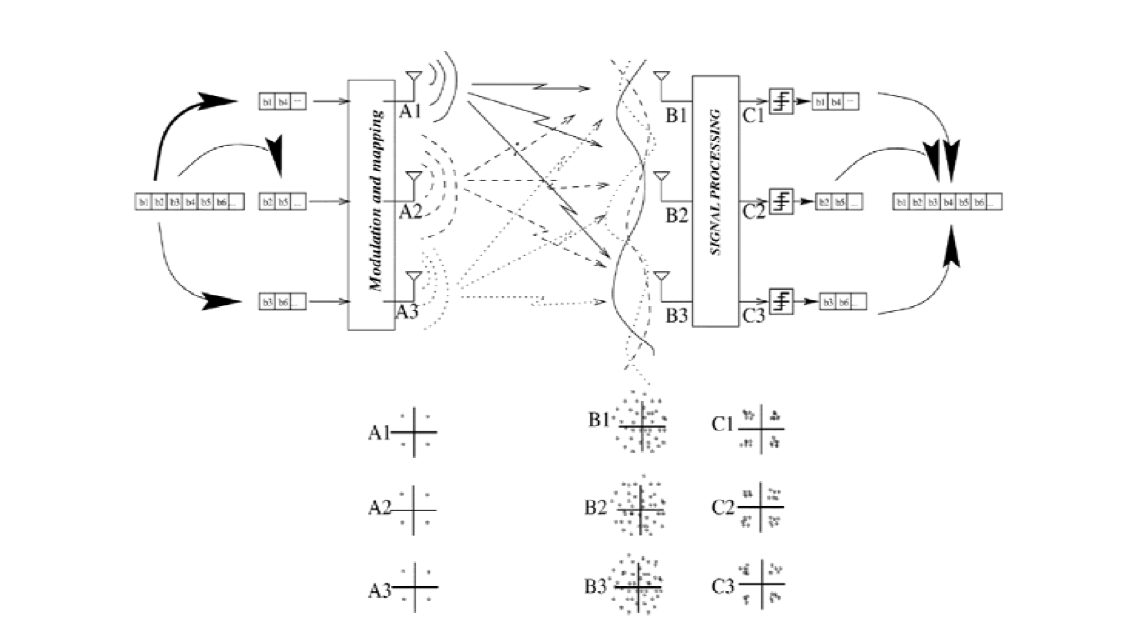
\includegraphics[width=13cm]{./figures/C02-spatial_multi_1}
%         \caption{Spatial Multiplexing con tres antenas en transmisor y receptor}
%         \label{fig:spatial_multi1}
% \end{figure}
% 
% El proceso de dividir la secuencia de información en subflujos es realizado por un demultiplexor. El proceso de demultiplexado debe ser aplicado a bits o símbolos. Luego, la codificación puede ser realizada en tres formas diferentes de acuerdo a la posición del demultiplexor en la cadena del transmisor y la dirección de la capa. Estos procesos de codificación son referidos como horizontal, vertical y diagonal. Las distintas técnicas de codificación se muestran en la figura \ref{fig:spatial_multi2}.
% 
% \begin{figure}[htb!]
%         \centering
%         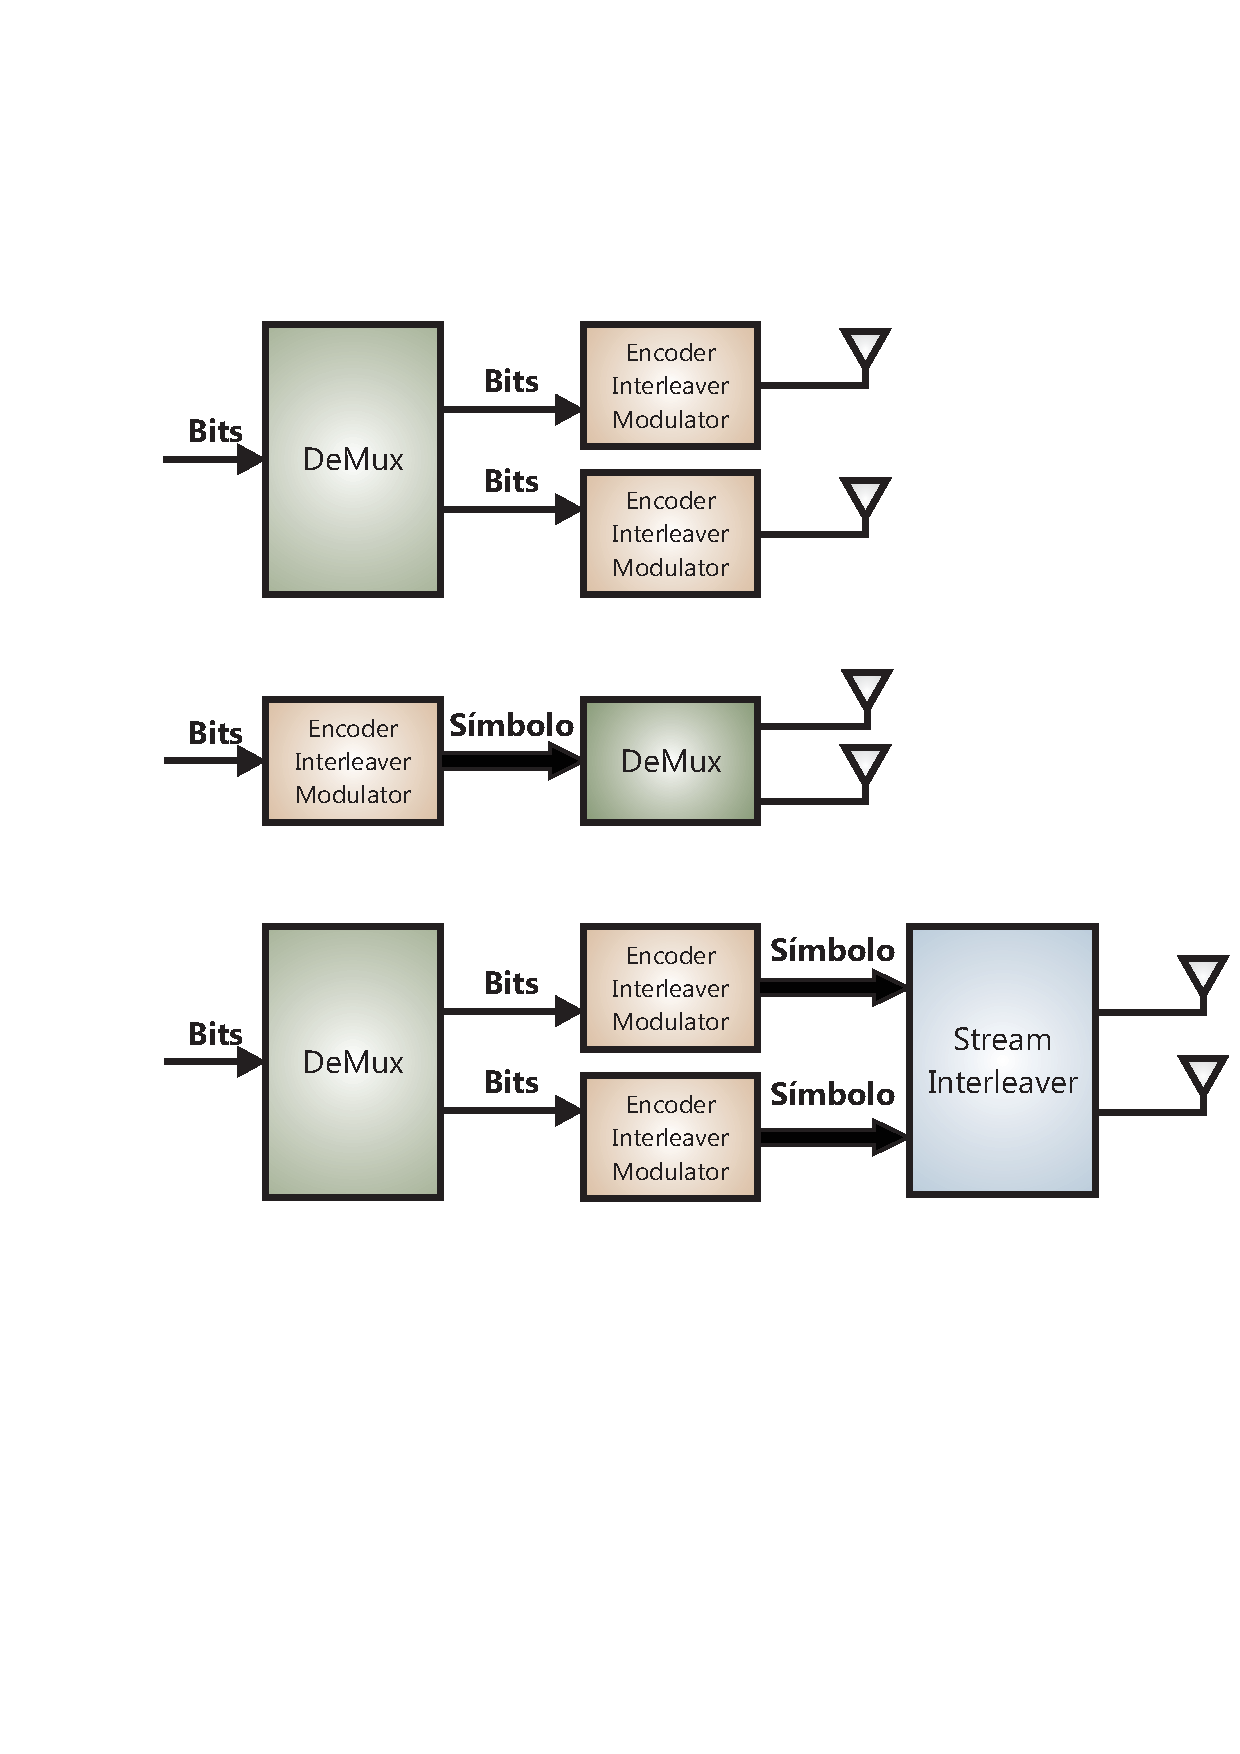
\includegraphics[width=9cm]{./figures/C02-spatial_multi2}
%         \caption{Tipos de codificación para Spatial Multiplexing}
%         \label{fig:spatial_multi2}
% \end{figure}
% 
% \newpage
% 
% En el codificado horizontal, los bits de datos son demultiplexados en $M_T$ subflujos que son independientemente codificados, intercalados y modulados. Por otro lado, en la realización vertical, el flujo de datos es codificado, intercalado y modulado; y, los símbolos resultantes son luego demultiplexados en $M_T$ subflujos. El proceso para realizar spatial multiplexing diagonal es similar al codificado horizontal, con la única difrerencia de que, luedo de la etapa final, los frames de símbolos son sometidos a un intercalado de flujo, el cual rota los frames transmitidos.